\documentclass[a4paper]{report}

\usepackage{altgraphicx}
\usepackage{amsmath}
\usepackage[english]{babel}
\usepackage[backend=biber,style=apa]{biblatex}
\usepackage{color}
\usepackage[utf8x]{hyperref}
\usepackage[utf8x]{inputenc}
\usepackage{listings}
\usepackage{svg}

\graphicspath{{./assets/figures/}{./assets/images/}}

\addbibresource{bibliography.bib}

% Code formatting.
\definecolor{lstcodebackground}{rgb}{0.95, 0.95, 0.95}
\definecolor{lstcodecomment}{rgb}{0.5, 0.5, 0.5}
\definecolor{lstcodekeyword}{rgb}{0.60, 0.15, 0.70}
\definecolor{lstcodestring}{rgb}{0.55 ,0.75, 0.30}
\definecolor{lstcodenumber}{rgb}{0.0, 0.65 , 0.95}
\definecolor{lstcodelinenumber}{rgb}{0.5, 0.5, 0.5}

\lstdefinestyle{cinematiccolor}{
    backgroundcolor=\color{lstcodebackground},
    commentstyle=\color{lstcodecomment},
    keywordstyle=\textbf\color{lstcodekeyword},
    numberstyle=\color{lstcodelinenumber},
    stringstyle=\color{lstcodestring},
    basicstyle=\footnotesize,
    breakatwhitespace=false,
    breaklines=true,
    captionpos=b,
    keepspaces=true,
    % numbers=left,
    % numbersep=5pt,
    showspaces=false,
    showstringspaces=false,
    showtabs=false,
    tabsize=4
}

\lstset{style=cinematiccolor}

\title{
    {\LARGE Color for Motion Pictures and Games}
    \\
    \vspace{5mm}
    {\large From Design to Display}
}

\begin{document}

\maketitle

\begin{center}
    {\LARGE A VES Technology Committee White Paper}
    \\
    \vspace{5mm}
    {\large 2018-2019}
\end{center}

\chapter*{Foreword}

\section*{Description}

This updated paper presents an introduction to color management for motion-picture, television and games production, including visual effects, animation. It expands on the original’s focus on motion-picture visual effects and animation as a reflection of the expanded scope of digital imaging in the film and television production process, from capture to post-production to grading and final display, and as a reflection of the consistency in basic approaches used by visual effects, animation and increasingly games projects.

Color impacts many areas of the movie and the game-making process. From on-set capture to the many phases of the computer graphics pipeline: texture painting, look development, lighting, rendering, and compositing, to grading and finishing for the theater and home. Handling color is a tricky problem. This paper presents an introduction to color science, measuring and encoding color and core concepts like gamuts, transfer functions, and scene-referred and output-referred colorimetry. The paper then extends these concepts to their use in modern motion-picture and games production, including an introduction to efforts on digital color standardization in the motion-picture industry, ACES and ASC CDL, and how readers can experiment with all of these concepts for free using open-source software like OpenColorIO and Colour Science for Python.



\section*{Authorship}

The updated paper was authored by Alex Forsythe, Alex Fry, Stefan Luka, Thomas Mansencal, Kevin Shaw and Nick Shaw. 

The paper continues to include much of Jeremy Selan’s original text.

The update was edited by Haarm-Pieter Duiker.

The update was reviewed by members of the VES Technology Committee and others, including ...

The original paper was authored by Jeremy Selan and reviewed by the members of the VES Technology Committee including Rob Bredow, Dan Candela, Nick Cannon, Paul Debevec, Ray Feeney, Andy Hendrickson, Gautham Krishnamurti, Sam Richards, Jordan Soles, and Sebastian Sylwan.



\section*{On the Web}

The VES Technology Committee has assembled an expert panel that can be reached at ves-tech-color@googlegroups.com for questions, comments, and errata related to this document.

Visit CinematicColor.org for additional resources related to motion-picture color management.




\tableofcontents

\chapter{Introduction}

\section{Intended Audience}

This document is intended for professionals involved in the capture, production and finishing of film, animation, and games, with a particular focus on the computer graphics artists and software developers responsible for visual effects, animation and games color management. A familiarity with computer graphics fundamentals is assumed. As advanced color imaging techniques, like wide color gamut and high-dynamic range capture, processing and display, become more widely used outside of the entertainment space, we expect that this paper will also be relevant to professionals beyond the intended audience. A familiarity with color science and color management is not.



\section{How to Read this Document}

The paper is broken into this Introduction, sections on Color Science and Workflow and an Appendix. The ordering of the content should introduce a reader new to the subject to the concepts and terminology needed to understand successive topics. For those focused on specific production workflows or challenges, it is reasonable to follow from the Introduction to Workflow, referring to Color Science, as needed. The Appendix provides more applied examples and explanation where it was deemed appropriate.



\section{The Goal}

Professionals in the motion picture, visual effects, animation, and games industries encounter color management challenges which are not covered in either traditional color science textbooks or online resources, leaving digital artists and computer graphics developers to fend for themselves. Best practices are too often maintained through tribal knowledge: passed along by word of mouth, user forums, or scripts copied between facilities. This document’s goal is to provide a better mechanism for communicating this information.

The paper also outlines the color pipeline challenges in modern feature film, visual effects, animation and games production, from on-set capture to the computer graphics pipeline to digital intermediate (DI) grading and final display. It presents techniques and best practices currently in use at major production facilities and notes areas that need further development and standardization.

One note to begin with: Color pipelines are not static nor is there a single best approach. They grow and evolve with the constraints of each project. This paper intends to present color measurement, processing, and pipelines in enough generality that the reader will be able to address the specific needs of their productions, even if they are not described explicitly in the text. It is unlikely that this paper will address the exact requirements of any given production in whole.



\section{Converging Approaches}

Figure 1. A high-level element breakdown for live-action, mixed live action, animation and games shots. Each image is generated using a roughly consistent set of stages and processing steps. The succession of image states is as follows: 1) Camera image, in camera-native color space 2) Ungraded camera image or renderer output in an ungraded working color space 3) Image with generic grade 4) Final graded image for primary output with composited background and foreground elements and 5) graded image for an alternate output like PQ or DCDM. The terms used here are defined later in this document.
Images are © Geoff Boyle  © 2018 MARVEL, © Disney/Pixar,  © Disney 2018. Imagery from Battlefield V courtesy of Electronic Arts Inc, © 2018 Electronic Arts Inc. All rights reserved.

Since the first version of this document, there has been a convergence of approaches across cinematography, visual effects, animation, games, finishing, and grading. Shared challenges in the evolution of display and capture technology: a shift from photochemical to digital image capture, widely available wide-gamut high-dynamic range (HDR) displays, advances in rendering and image generation research and the increased integration of different production departments have driven this harmonization. Each production will define a slightly different overall color pipeline, but most discussion, debate, and variation boils down to choices made around the transforms and formats used. Image and color data with specific meaning, referring to scene or display intensities, and transforms, with specific expectations for input and output format, are concepts that are used remarkably consistently across on-set capture, visual effects, games, finishing, grading and software and hardware color processing pipelines.

Figure 1 above shows a consistent set of image states leading towards the final frame for live action, live-action with integrated visual effects, fully synthetic visual effects images, animated features, and games.



\section{A General Model of Color Processing}

Digital color management follows a clear general path tightly coupled with digital imaging. The high-level diagram below covers this path, from reflectance, image formation, storage and processing to display.

The ‘Computer Graphics’ box hides a complex pipeline that largely mimics the physical processes that precede it in this diagram, with the goals of creating content that will blend seamlessly with the captured image. Key: Purple - physical light, Blue - stored light, Green - Synthetic light, Orange - perceived light

While there are many imaging considerations along the full imaging pipeline, such as spatial and temporal considerations, this discussion restricted itself to the propagation and transformation of color in the imaging pipeline.

The simplest example of the digital color pipeline for cinema is exemplified by a digital camera, covering the full imaging pipeline from lens to sensor to the display on the back of the camera. Even this simplest case involves processing and transforms that are a microcosm of more complex pipelines. From this example, it is possible to expand to cover pipelines and workflows that have processing steps in-camera, on-set, in a scanning house, with editors, in a renderer, visual effects, animation and games teams, colorists, distribution processing, cinemas, streaming services and everywhere in between. In this section, the paper will present simple models for thinking about color processing and understanding which aspects are important in each phase of production.

In the simple case mentioned above, an image captured by a digital camera and displayed on the screen on the back of the camera, there are a series of states and transforms to consider:
Light reflected off a surface, into camera’s lens and onto an image sensor
Sensor photosite values encoded and stored in memory
A transform to combine adjacent Red, Green and Blue photosites into single pixel values
A “working space” image in memory
A transform to remap the intensities of the combined pixels for display
A “displayable” image ready to be sent to the display hardware
The display hardware showing the image


Optical diagram of a typical mirrorless digital camera.
Unknown. (n.d.). DSLR Optical Diagram. Retrieved October 14, 2018, from https://www.dpreview.com/forums/post/61693925

The aspects of the example above that will show up repeatedly throughout this document are:

Input, Working, Output: The example includes the stages that are common to most modern color pipelines, namely an Input, Capture or Generated image state, a Working image state used for editing and production and an Output image state used for display. There may be other steps along the way, but virtually all modern color pipeline designs contain these three distinct states. The Input image for a visual effects or animated feature or game may be the product of a renderer.

Scene-referred, Output-referred images: The sensor image in Step 3 represents the intensity of light in the scene, filtered through the camera’s lens and specific red, green and blue filters over each sensor photosite. The “working space” image from Step 5 also represents the intensity of light in the scene, but may be device-independent, at least slightly abstracted from the camera sensor and processing hardware. After being transformed for display, the image in Step 6 has values representing the activations necessary for each of the target display’s pixels.

Transforms - Input, Output, Look: Going between each image state is a transformation that has a specific, meaningful effect. The most widely used transforms will typically include a remapping of intensities and some degree of remapping of the color gamut: the underlying meaning of the red, green and blue of each pixel. There are many more exotic transforms, and often a number of these simpler transforms are concatenated. Transforms going from Input to the Working space are usually strictly defined based on the capabilities of the capture device and the attributes of the working space. Transforms from the Working space to the Output space usually combine an element of artistry, commonly referred to as “the Look”, with an explicit mapping based on the capabilities of the output device. Later sections of the document contain many examples of transforms used in practice.

Staged Processing: The process to go from light hitting the sensor to a display emitting light is defined by a specific, staged processing pipeline. Transforms take color from one image state to the next, constrained by the processing needs of each successive stage and the limitations and capabilities of the capture, processing and display hardware. Images may be written to disk or passed along an IO line representing the state of color at any of the points in the processing chain, as different applications or departments within production may be the source or the destination for the data.

Meaning and Placement - Understanding how to work with an image or color data set is more natural when you can be clear about what the data is supposed to represent and where it lives in the production or product’s processing chain. These two elements, meaning and placement, provide the context needed to apply transformations and make aesthetic judgements in production.

\subsection{ACES}

The Academy Color Encoding System (ACES) is a color management system that embodied the general model of color processing described above. It codifies and standardizes many of the elements described in the Workflow section with an eye towards addressing many of the difficulties listed in the Challenges section below. The basic system diagram for ACES is presented below.


ACES system diagram

This diagram contains scene-referred imagery, transforms converting from one state or color space to the next, working spaces, output-referred imagery and an ordered, staged processing pipeline.

ACES is one of many ways to define a color pipeline, but it presents a nice embodiment of the general model of color processing presented above, mirrored in most of the examples discussed in this paper. ACES will be referenced throughout this document because it is open, well documented, widely available and has been used successfully in a wide variety of projects of all types and complexities. It provides a great starting point for exploration. This should not be taken as a suggestion that ACES is the only or necessarily the best option. Decisions about which color transforms and spaces to use should be base on the requirements and constraints of a given project.



\section{Color Management Challenges}

While the approaches in different industries and departments have converged, there are still many challenges when speaking about and working with color. They are:

Multiple Requirements: It is difficult to lump on-set capture, visual effects, animation, games, grading and finishing into a single bucket, as each discipline has potentially different color pipeline goals and constraints. For example, in visual effects production, one of the golden rules is that image regions absent of visual effects should not be modified in any way. This places a constraint on color pipelines: that color conversions applied to the photography must be perfectly invertible. Animation and games have their own unique set of requirements, such as high-fidelity handling of saturated portions of the color gamut along with large areas of smooth color gradients. On-set capture teams are focused on a shot to shot consistency, capturing as much dynamic range with as little noise as possible. Grading teams have to deliver a set of final images that retain the intended look and feel of the production and take maximum advantage of the output device(s), standard dynamic range (SDR) and high-dynamic range (HDR). Thus, color pipelines must keep track of the “big picture” priorities but are often tailored to specific productions and groups.

Varying Terminology: Working with color in a single production setting can be a challenge. An additional complicating factor is the abundance of overlapping and overloaded terminology for describing color and operations on color. As more parts of the production pipeline interact, from on-set capture to visual effects to grading and mastering, the history, and constraints that defined how each group thinks and talks about color come in contact when they may not have previously. Terms like grade, HDR, linear, brightness, gamma, light, look development or LUT may have clear, but different, meanings in two adjacent production groups. On top of overloaded terms, many acronyms in use add a level of perceived complexity to what would otherwise be an easily understood process. The Glossary in the Appendix is our attempt to address some of this overloading of terms.

Various Color Philosophies: There are many schools of thought on how to best manage color in digital motion-picture production. There is far more variation in motion-picture color management than in desktop publishing. Some facilities render in high-dynamic range (HDR) color spaces. Other facilities prefer to render in low-dynamic range (LDR). Some facilities rely on the output display characteristics, like gamma, as the primary tool in crafting the final image appearance. Others do not. It is challenging to provide standardized workflows and toolsets when the current practice has such variation.

Multiple Inputs & Outputs: In live-action productions, imagery is often acquired using a multitude of input capture devices: multiple digital motion picture cameras from different vendors, still cameras, “action cameras,” specialized HDR panorama cameras, LIDAR scanners, and it is desired to merge these different sources seamlessly. On the output side, the final image deliverables are tailored to distinct viewing environments: digital theatrical presentation, film theatrical presentation, SDR and HDR home theater, television broadcast, augmented and virtual reality devices. The rapid evolution of HDR display’s brightness and color gamut standards poses particular challenges for content creation and grading. Each of these outputs has different color considerations. Furthermore, artists often work on desktop displays with “office” viewing conditions, yet require a high-fidelity preview of the final appearance.

Complex Software Ecosystem: Another challenge is that the majority of the motion picture, visual effects, animation and games productions use many software tools: on-set monitoring, LUT boxes, image viewers, 2D and 3D painting applications, compositing applications, lighting tools, editing and grading suite, media generation and transcoding software  and so on. Although it is imperative that artists work in a color managed pipeline across multiple applications, color support is quite varied between software vendors. Ideally, all software tools that interchange images, perform color conversions or display images should be color managed consistently. This is not the case. Each production and facility has to understand the capabilities and behavior of the applications they elect to use as part of their pipeline design. The issue of interchange takes on an even more complex angle when you consider that multiple facilities often share image assets on a single production. Color management practices and technologies that encourage high-fidelity, consistent interchange are sorely needed.

Protecting Imagery: On-set capture, visual effects, and animation are not the end of the line for image processing. Digital intermediate (DI) Grading is a powerful tool for crafting the final appearance of a motion picture that may substantially impact the appearance of the final image. It is, therefore, a necessity for on-set capture and post-production color pipelines to protect the fidelity of the captured and rendered image, even under drastic color corrections. It is very likely that late stage color corrections will reveal underlying problems in the captured or computer-generated imagery if digital intermediate is not considered earlier in production. Artifacts not visible in production because of the viewing conditions or introduced by changes made in post-production might be very obvious in HDR or at 2 stops less exposure. The eventual application of compression is also a consideration.
Future-Proofing Required: Display technology is continually evolving, most recently with high resolution (UltraHD), wide color gamut (Rec. 2020) and higher dynamic range (Rec. 2100). For large productions, it is very prudent to take all steps possible to future-proof the computer-generated (CG) imagery so that visual effects (VFX) elements can be repurposed and do not need to be recreated when the next generation of display technology appears. It is good practice to work and archive at the source resolution. Color space, bit depth, and dynamic range should also be protected. These requirements can be very demanding of storage, bandwidth and processing power in modern times, often resulting in the use of compression algorithms to ease the strain. Some of these may be visually lossless yet still impact the color pipeline in the later stages.



\chapter{Color Science}

\section{About Color Science}

Color science is the scientific domain studying the human perception of color, its measurement, and characterization. Terminology in a scientific field is critical to understanding that field and precisely discussing its concepts. Color is ubiquitous in our lives but typically not well understood.

Mark D. Fairchild writes:
“Almost everyone knows what color is. After all, they have had firsthand experience of it since shortly after birth. However, very few can precisely describe their color experiences or even precisely define color.”

The International Commission on Illumination (CIE) defines perceived color as the “characteristic of visual perception that can be described by attributes of hue, brightness (or lightness) and colo(u)rfulness (or saturation or chroma).”

This document is necessarily an overview of color science. The foundational texts listed below can provide a deeper understanding.
Digital Color Management: Encoding Solutions, 2nd Edition by Madden and Giorgianni (2007) provides an in-depth analysis of the nature of color images, digital color encoding, color management systems and digital color interchange.
Color Appearance Models by Fairchild (2013) is the reference for the fundamental concepts and phenomena of color appearance.
The Reproduction of Colour (6th ed.) by Hunt (2004) describes the fundamental principles of colorimetry, color appearance, color reproduction for photography, television, printing and electronic imaging.
Digital Video and HD, Second Edition: Algorithms and Interfaces by Poynton (2012) details the theory and engineering of digital video systems.
Color Science: Concepts and Methods, Quantitative Data and Formulae by Wyszecki and Stiles (1982) is the authoritative reference for colorimetry.
The authors of this paper are greatly indebted to the writers of these books.

Dr. Robert W.G. Hunt passed away during the writing of this section. His work is foundational to the color science community. Dr. Hunt’s contributions to the understanding of human color perception and its application to the engineering of photographic systems laid the foundation for much of the color science that is used in the motion picture and gaming industries today. Besides being a brilliant scientist, Dr. Hunt was a kind man always willing to share his knowledge, whether formally in one of the many classes he taught, or informally over coffee or a meal. Dr. Hunt’s true passion was teaching others. A few of the authors of this document had the good fortune to have known and learned from Dr. Hunt and were saddened to hear of his passing. His contributions to the field, friendship and mentorship will be missed.

A tribute to Dr. Robert W.G. Hunt: Light dispersion through a prism (bottom right) with the rainbow of color components lighting up The Reproduction of Colour (6th ed.) by Hunt (2004).

Color management depends fundamentally on colorimetry, the measurement of color. Without colorimetry, it is not possible to characterize cameras and displays or understand the imaging principles that permeate the rest of computer graphics. While it is possible to immediately dive into color pipelines, having a rudimentary understanding of concepts such as spectral measurement, tristimulus values, or color appearance provides a richer understanding of why some approaches to color management are successful, and some are not.

This section endeavors to stay generic and abstract. It does not focus on particular workflow details but provides the necessary foundations for understanding section 3. This section abundantly references the history of color science because the understanding of the past is essential for the comprehension of the present: knowing how colorimetry evolved explains the current practices. The physical nature of light and the quantities used for its analysis are examined. The anatomy of the human visual system (HVS) is reviewed with a particular focus on the eye and the primary adaptation mechanisms. Basic colorimetry is presented, providing the requisites for converting spectral measurements to RGB values or understanding perceptual uniformity. Advanced colorimetry, the gateway to color appearance modeling, is summarily exposed. Then, the representation of color is described, driving the section toward concrete concepts in direct relation with motion pictures color management. Finally, color imaging systems and the image capture, signal processing, and image formation stages are explained using digital imaging devices such as motion pictures cameras or LCD displays.

Key Points
Color science studies the human perception of color, its measurement, and characterization.
Proper terminology usage is critical to the understanding of a scientific field.
Color is the characteristic of a visual perception.
Color management depends on colorimetry, the measurement of color.


\section{Electromagnetic Spectrum}

Color is a perceived sensation that occurs when light interacts with the HVS. The CIE defines light as the “electromagnetic radiation that is considered from the point of view of its ability to excite the human visual system.”

The electromagnetic spectrum from approximately 360-780 nm is visible to human observers and called the visible spectrum. Note that color sensations produced above are limited to those the particular display used to view this document can represent.

In Opticks, Isaac Newton (1704) investigates the fundamental nature of light and color by describing the refraction of light by prisms. Newton demonstrated that a prism can separate seemingly achromatic light into components perceived as distinct hues, with each hue refracted at a unique and consistent angle; that this separated light may be recombined, either entirely to recover the achromatic color, or selectively, by which he could produce any desired color sensation.

Comparison of an original scene on the left and a version where its light is dispersed horizontally with a Star Analyser 100 (SA-100) diffraction grating demonstrating that the seemingly white light from the Sun illuminating the scene is composed of distinct hues.

Newton asserted that color is a visual sensation and not an inherent property of the light or object materials. He supported this assertion by noting that a magenta (purple) sensation can be created by combining red and violet components of two spectra, but this sensation is not produced by any single component of refracted light.

The measurement of the radiation across the entire electromagnetic spectrum is known as radiometry. In this document, the focus is almost entirely on radiation within the visible spectrum. Photometry is a subset of radiometry concerned solely with radiation within the visible spectrum, where the measurement of energy at a particular wavelength in that spectrum is weighted by the sensitivity of the HVS at that wavelength. A comprehensive description of radiometry and photometry is beyond the scope of this document, but the next sections define some necessary radiometric and photometric quantities used in digital imaging and color science. Their descriptions below are taken from Wyszecki and Stiles (2000).

\subsection{Radiometric Quantities of Interest}

Radiant power (or radiant flux) (Pe) is radiant energy emitted, transferred, or received through a surface, in a unit time interval. 

It has a unit of Watt (Joules.sec-1).
Irradiance (Ee) at a point of a surface is the quotient of the radiant power incident on an infinitesimal surface element containing the point, by the area of that surface element. It has a unit of Watt.m-2.
Radiance Exitance (or radiosity) (Me) at a point of a surface is the quotient of the radiant power emitted by an infinitesimal surface element containing the point, by the area of that surface element. 

It has a unit of Watt.m-2. 
Radiance Intensity (Ie) of a source in a given direction is the quotient of the radiant power emitted by the source in an infinitesimal element of solid angle containing the given direction by the element of solid angle. 

It has a unit of Watt.sr-1.
Radiance (Le) in a given direction at a point on the surface of a source or a receiver, or at a point on the path of a beam, is the quotient of the radiant power leaving, arriving at, or passing through an element of surface at this point and propagated in directions defined by an elementary cone containing the given direction, by the product of the solid angle of the cone and the area of the orthogonal projection of the surface element on a plane perpendicular to the given direction. 

It has a unit of Watt.m-2.sr-1.

\subsection{Photometric Quantities of Interest}

Photometric quantities
Luminous power (or luminous flux) (Pv) is the quantity derived from radiant power by evaluating the radiant energy according to its action upon a selective receptor, the spectral sensitivity of which is defined by a standard luminous efficiency function. 

It has a unit of Lumen (lm.sec-1).
Illuminance (Ev) at a point of a surface is the quotient of the luminous power incident on an infinitesimal element of the surface containing the point under consideration, by the area of that surface element. 

It has a unit of lm.m-2 (or Lux).
Luminous Exitance (or luminous emittance) (Mv) from a point on a surface is the quotient of the luminous power emitted from an infinitesimal element of the surface containing the point under consideration, by the area of that surface element. 

It has a unit of lm.m-2 (or Lux).
Luminous Intensity (Iv) in a given direction is the quotient of the luminous power emitted by a point source in an infinitesimal cone containing the given direction, by the solid angle of that cone. 

It has a unit of candela (cd).
Luminance (Lv) at a point of a surface and in a given direction is the quotient of the luminous intensity in the given direction of an infinitesimal element of the surface containing the point under consideration, by the orthogonally projected area of the surface element on a plane perpendicular to the given direction. 

It has a unit of cd.m-2. A convenient non-SI (International System of Units) shorthand for the luminance unit is nit from the latin nitere, to shine.
Relative Luminance (Y) is luminance normalized to the range 0-1 or 0-100, relative to a reference white Luminance value.
Key Points
Color is perceived when light interacts with the HVS.
Light is the visible portion of the electromagnetic spectrum.
Achromatic light can be separated into distinct hues by prisms. Those distinct hues can be recombined by prisms to recover the achromatic light.
Color is not an inherent property of the light or object materials:  magenta does not exist as a distinct hue but is perceived when combined red and blue hues.
Radiometry is the measurement of radiation across the entire electromagnetic spectrum.
Photometry is the measurement of radiation weighted by the sensitivity of the HVS across the visible spectrum.

\subsection{Spectral Distribution}

In radiometry and photometry, the radiant power emitted by a light source or illuminant, or reflected, transmitted or absorbed by a surface is characterized by a spectral distribution giving the power of the light per unit area per unit wavelength or the percentage of light reflected, transmitted or absorbed per unit wavelength.


Four CIE illuminants spectral power distributions. A and D65 are respectively CIE Standard Illuminant A and CIE Standard Illuminant D65 and are described in section 2.3.4. F2 is CIE Illuminant F2, a fluorescent type light and HeNe Laser (Normalised) is a Helium-Neon laser measured by Deglr6328 (2006).

The visible spectrum is considered for electromagnetic radiation with wavelengths in the range of approximately 360-780 nanometers (nm). The spectral sensitivity of the human eye peaks under daylight-like illumination towards the middle of this range, at 555nm (yellow-green). At the extremes, radiant energy below 360nm (ultraviolet)  or above 780nm (infrared) appears indistinguishable from black, no matter how intense.


Reflectance, transmittance and absorptance spectra of a Sorghum Halepense leaf from LOPEX93. Chlorophyll absorbs a large quantity of blue and red radiation giving leaves their green color.
Light, through its fluctuations and spectral quality, has contributed to shaping the adaptation of many species. Chlorophyll, contained in plants chloroplasts, is a pigment which absorbs light during photosynthesis. It absorbs violet, blue and red wavelengths while reflecting green wavelengths. 

Sparks, DasSarma, and Reid (2006) and DasSarma and Schwieterman (2018) have proposed the hypothesis that early photosynthetic organisms may have used retinal pigment which has a peak absorption centered at 550nm, thus absorbing most of the green wavelengths. The chlorophyll based organisms that appeared later adapted by absorbing the remaining regions of the electromagnetic spectrum.



Solar spectral irradiance compared to CIE 1924 Photopic Standard Observer, note how both peak around 555nm.

The solar spectral irradiance is thought to be a fundamental driver of the evolution of the HVS and peaks in the central region of the visible spectrum. Boynton (1990) says that "this coincidence is probably not accidental, but is more likely the product of biological evolution." Wang, Tang, and Yan (2011) have shown that the spectral sensitivities of photoreceptors of different species of moray eel were correlated with the photic characteristics of their habitats.

Key Points
A spectral distribution characterizes, at each wavelength, the radiant power emitted by a light source or the percentage of light reflected, transmitted or absorbed by a surface.
The wavelengths range of the visible spectrum is approximately 360-780nm.
Spectral sensitivity of the HVS peaks at 555nm, ultraviolet radiation below 360nm or infrared radiation above 780nm is invisible.
The solar spectral irradiance peaks in the central region of the visible spectrum and is thought to be an essential driver of the evolution of the HVS.




\section{Human Visual System}

Visual perception, a process by which humans acquire knowledge about their environment, is initiated when environmental light enters the eye and induces electrical signals subsequently processed within the brain where an image is formed. Acquiring knowledge is a cognitive process distinct from strict optical mechanisms. There are optical similarities between a camera and the eye in the way they capture an image of the environment but a camera does not have perceptual capabilities or cognitive abilities; it does not know about the world.

The principal components on the visual pathway are as follows:
Eye
Optic nerve
Optic chiasma
Optic tract
Lateral geniculate body
Optic radiation
Visual cortex
Visual association cortex

Principal components of the human visual system.
Wikipedia. (n.d.). Human visual pathway. Retrieved October 14, 2018, from https://commons.wikimedia.org/wiki/File:Human_visual_pathway.svg

Their study is beyond the scope of this document but it is important to highlight that while the light from the environment is captured and converted to electrical impulses by the eye, most of the information extraction happens in the cerebral cortex and multiple interpretations of the sensory stimulation are possible. 

Rotating snakes: Circular snakes appear to rotate spontaneously.
Kitaoka, A. (2003). Rotating snakes. Retrieved October 14, 2018, from http://www.ritsumei.ac.jp/~akitaoka/rotsnake.gif

Optical illusions are the result of light stimuli producing ambiguous and conflicting interpretations. They are important because they demonstrate that the stimulation of the eye does not entirely determine perception. Our perceptions correspond to the models the HVS has constructed rather than the original sensory stimulation. Palmer (1999) explains that "the observer constructs a model of what environmental situation might have produced the observed pattern of sensory stimulation." 
Key Points
Visual perception allows human to acquire knowledge about their environment.
Knowledge acquisition is a cognitive process.
Camera and the eye have optical similarities, but a camera does not have cognitive abilities.
Most of the information extraction happens in the cerebral cortex.
Optical illusions demonstrate that eye stimulation is not solely responsible for our perceptions: the HVS constructs a best-fitting model of the environmental situation.

\subsection{The Eye}

The eye is of particular interest being the sensor with which the HVS probes the environmental light.

Cross section of the human eye.
https://commons.wikimedia.org/wiki/File:Eyesection.svg

The light pathway through the eye starts at the cornea, a transparent and curved organized group of tissue layers. The cornea represents the largest index of refraction (1.376) change at its interface with air. It contributes 3/4 of the eye focusing power although its focus is fixed.
Upon exiting the cornea, the light traverses the aqueous humor, a water-like fluid with a refractive index of 1.336, filling the anterior and posterior chambers of the eye and providing nutrition to the surrounding tissues.

Similar to a camera diaphragm, the iris, a ciliary muscle, controls the pupil size and therefore the amount of light reaching the retina. The pupil diameter varies from 7mm in dark viewing conditions to 3mm in bright viewing conditions

The light not absorbed by the iris enters the lens which provides the accommodation function (optical power change) by adjusting its shape allowing to focus at various distances. Its biconvex shape becomes flattened thus decreasing optical power to focus at a distance and fatter to increase optical power to focus at nearby objects. Its refraction index varies from edges to center (1.386 to 1.406) to reduce chromatic aberration.

The light traverses the vitreous humor, a thick fluid with a refractive index of 1.336, filling the space between the lens and the retina, to finally reach the retina.

Key Points
The eye is the HVS light sensor and is analogous to a camera.
Light enters the HVS through the cornea, the eye element with the strongest focusing power.
The iris controls the amount of light reaching the back of the eye by changing the pupil diameter akin to a camera diaphragm.
The lens allows the eye to focus on objects at varying distances by changing its shape, i.e. accommodation.

\subsection{Retina}

The retina is a light-sensitive tissue composed of layers of neurons connected by synapses and receiving the optical image formed by the front eye elements. It contains the photoreceptor cells, the initial signal processing and transmission elements of the HVS.

We move our head and eyes so that the image of objects we look at falls on the fovea, a 1.5mm central pit area of the retina with increased density of photoreceptor cells and responsible for high-resolution vision.

Light traverses almost all the retinal layers before reaching the photoreceptor cells. Light triggers chemical changes in the photoreceptor cells which in turn, send a signal to the bipolar and horizontal cells. The signal is then propagated to the amacrine cells and ganglion cells, and finally to the optic nerve. 


Each synapse between the neural cells can perform an arithmetical operation such as amplification, gain control or nonlinear mapping, giving the eye the ability to perform spatial and temporal optical image sharpening.


The retina layers.
https://commons.wikimedia.org/wiki/File:Retina_layers.svg - colour-science.org

Key Points
The retina contains the photoreceptor cells, the initial signal processing and transmission elements of the HVS.
The fovea is a central retinal area with increased photoreceptor cells density, our heads and eyes are moving so that objects images fall on it.
Neural cells perform optical image sharpening.

\subsection{Photoreceptors}

The photoreceptors are a type of neuron specialized for phototransduction, a process by which light is converted into electrical signals. There are two main classes of retinal photoreceptors:
Cone cell
Rod cells
The third class of photoreceptor cells within the retina is the Intrinsically Photosensitive Retinal Ganglion Cells (ipRGC) which play a significant role in the modulation of circadian rhythms, pupillary response, and adaptation.

\subsubsection{Cones and Photopic Vision}

Cone cells mediate photopic vision, which is vision under daytime illumination conditions, and are responsible for color perception. In the photoreceptor layer of the retina, cone cells of types L, M, S (sensitive to Long, Medium and Short wavelengths respectively) measure light with respective peak absorption at wavelengths of about 564 nm, 534 nm, and 420 nm.

Photopic vision luminance levels are usually defined for Luminance > 10 cd/m2.

The long, medium, and short cone fundamentals for 2 degrees showing respective peak absorption at wavelengths of about 564 nm, 534 nm, and 420 nm.

Most humans possess L, M, and S cone cells with similar distributions and peak absorptions, however a significant part of the population is affected by some form of color vision deficiency or color blindness. The most common types are:
Protanomaly: Defective L cone cells; the complete absence of L cone cells is known as Protanopia or red-dichromacy.
Deuteranomaly: Defective M cone cells with peak of sensitivity moved towards the red sensitive cones; the complete absence of M cone cells is known as Deuteranopia.
Tritanomaly: defective S cone cells, an alleviated form of blue-yellow color blindness; the complete absence of S cone cells is known as Tritanopia.
Monochromats only carry a single type of cone cells.
Tetrachromats carry four types of cone cells.

\subsubsection{Rods and Scotopic Vision}

The rod cells mediate scotopic vision, which is vision under dark illumination conditions and where rods are the principle active photoreceptors. They measure light with peak absorption at a wavelength of about 507 nm.

Scotopic vision luminance levels are defined for Luminance < 0.001 cd/m2. The rod cells are about 100 times more sensitive to light than the cone cells.

\subsubsection{Mesopic Vision}
Mesopic vision is the result of the photopic vision and scotopic vision being active at the same time and occurs at low illumination conditions, and is usually defined for luminance in range 0.001 to 3 cd/m2.
CIE 1924 Photopic and CIE 1951 Scotopic Standard Observers. They are presented along with a Photopic Luminance Mesopic Luminous Efficiency Function modeling the sensitivity of the HVS for illumination levels between Photopic and Scotopic visions at 20% Photopic Luminance.

\subsubsection{Distribution}

The distribution of photoreceptors in the retina, note their total absence in the blind spot.
https://commons.wikimedia.org/wiki/File:Human_photoreceptor_distribution.svg

There are around 6.8×106 cones cells and approximately 110-125×106 rod cells in the retina. Cone cells are concentrated in the fovea and sparsely distributed in the peripheral retina. The asymmetry in the L, M and S cone cells distribution, the absence of S cone cells in the fovea centralis and their wide spacing into its periphery account for chromatic aberration. When the image is focused on the fovea centralis where reside the L and M cone cells, the S cone cells receive the shorter wavelength components. The axial chromatic aberration of the lens blur those components, thus a lower spatial resolution is required for the S cone cells.

No rod cells are located in the central fovea region, allowing for increased spatial acuity to be conveyed by the cone cells. The blind spot is a notable area without photoreceptors and where the ganglion cell axons leave the eye to form the optic nerve.

A single cone cell feeds its signals into a single ganglion cell while hundreds of rods pool their responses to feed into a single ganglion cell establishing a system of information compression between the photoreceptors and the optical nerve.

Key Points
There are two main classes of photoreceptor cells in the retina: cones and rods.
Cone cells are responsible for color perception, and photopic vision, the vision under daytime illumination conditions, with luminance levels defined for Luminance > 10 cd/m2.
Rod cells are responsible for scotopic vision, the vision under dark illumination conditions, with  luminance levels defined for Luminance < 0.001 cd/m2
Rod cells are about 100 times more sensitive to light than the cone cells.

\subsection{Dynamic Range}

From starlight luminance levels around 10-4 cd/m2 to sunlight luminance levels reaching 105 cd/m2 or over 109 cd/m2 for a direct Sun luminance measurement, our world exhibits a wide dynamic range. In this context, dynamic range is the ratio between the maximum and minimum measurable light quantity in a scene.

The dynamic range of the human visual system.

The dynamic range of the HVS is the ratio between the most luminous stimulus causing complete photoreceptors bleaching with no damage and the smallest detectable light stimulus. Hood and Finkelstein (1986) and Ferwerda, Pattanaik, Shirley and Greenberg (1996) report from 10-6 to 10 cd/m2 for scotopic light levels and from 0.01 to 108 cd/m2 for the photopic range. However, the HVS, like any capture imaging devices, is unable to perceive this full range at once. Only a fraction is observable simultaneously, inducing HVS adaptation to illumination level variations.

The simultaneous dynamic range or steady-state dynamic range is defined as the ratio between the highest and lowest luminance values at which objects are detected while being in a state of full adaptation. It is the range of stimulus intensities over which photoreceptors are able to signal a change. Kunkel and Reinhard (2009) performed a series of psychophysical experiments on a high dynamic range display and determined that the HVS simultaneous dynamic range spans a range of 12.3 stops (3.7 log10 units) under illumination conditions with an adapting field varying from 1.78 cd/m2 to 17.8 cd/m2. They also found that the upper detection threshold was higher when the HVS is adapted to a brighter environment and thus that the maximum display luminance should be increased accordingly.

In the context of motion pictures and games, it is useful to talk about dynamic range in terms of photographic stops, i.e. doubling or halving of luminance. Stops are calculated as the log2 of the test luminance relative to a reference luminance level.

Relative exposure in stops is the log2 of the luminance relative to some reference exposure level. Any normalization factor suffices for relative comparisons.

EV
-8
-3
-2
-1
-0.5
0
0.5
1
2
3
8
2^EV
0.004
0.125
0.250
0.500
0.707
1
1.414
2
4
8
256
Scene-referred exposure values are often referenced in units of stops (EV), as the range between values is large for direct numerical comparisons. For example, it is difficult to get an intuition for what it means to reduce the exposure of an image by a factor of 0.004, it is generally more intuitive to refer to the same quantity as "-8 stops".

Key Points
The dynamic range of a scene is the ratio between the maximum and minimum measurable light quantity.
The dynamic range of the HVS is the ratio between the most intense non-damaging luminous stimulus and the smallest detectable light stimulus.
The HVS, like cameras, only perceive a fraction of the full extent of its dynamic range simultaneously.
The HVS simultaneous or steady-state dynamic range spans over 12.3 stops; the upper detection threshold rises with a brighter environment and thus requires brighter displays.
Dynamic range is often expressed in stops, a doubling or halving of luminance.

\subsection{Adaptation}

The human visual system dynamically adapts to different illumination levels to improve the visual response. The three essential adaptation mechanisms of the HVS are:
Dark adaptation
Light adaptation
Chromatic adaptation

\subsubsection{Dark Adaptation}

Dark adaptation occurs when luminance level decreases. As a result of the lack of illumination, the observer’s visual system adapts to the stimuli and the visual sensitivity increases. Initially, upon entering a dark area, the cone cells’ sensitivity increases to reach full adaptation after around 10 minutes, when the rod cells’ sensitivity outperforms that of the cones, and complete adaptation is reached within 30 minutes.

A notable effect of the rod cells driving the visual system at low luminance level is that there is not enough light energy to be able to discriminate colors. Another notable effect,  the Purkinje Effect or Purkinje Shift, characterizes the HVS peak luminance sensitivity shift toward shorter wavelengths of the visible spectrum.

\subsubsection{Light Adaptation}

Light adaptation is similar to dark adaption, but instead, the visual sensitivity decreases with luminance level increase. The adaptation process happening when entering a bright area is faster than dark adaptation. The rod cells first saturate as rhodopsin the photopigment of the rods, photo-bleaches, while the cone cells continue to adapt reaching peak sensitivity within 5-10 minutes.

\subsubsection{Chromatic Adaptation}

The CIE defines chromatic adaptation as the "visual process whereby approximate compensation is made for changes in the colo(u)rs of stimuli, especially in the case of changes in illuminants".

Chromatic adaptation controls the independent sensitivity of the three cones cells type and is the most important adaptation mechanism in color appearance. A white object viewed under different lighting conditions (daylight, tungsten or incandescent lighting) retains its white appearance because the sensitivity of the cone cells is independently adjusted to compensate for the changes in energy level at the wavelength ranges they are sensitive to. Chromatic adaptation can be thought of as analogous to the automatic white balancing feature of a camera.

It is important to make a distinction between the adapted white, defined by the CIE as the "colour stimulus that an observer who is adapted to the viewing environment would judge to be perfectly achromatic and to have a luminance factor of unity" and the adopted white defined as the "spectral radiance distribution as seen by an image capture or measurement device and converted to colour signals that are considered to be perfectly achromatic and to have an observer adaptive luminance factor of unity; i.e., colour signals that are considered to correspond to a perfect white diffuser". The adopted white, used in the color imaging system, is specified and known while the adapted white of the HVS can only be estimated.

Chromatic adaptation occurs at a faster rate than dark and light adaptation. Rinner and Gegenfurtner (2000) measured two separate adaptation mechanisms representing 40% of the total adaptation for color appearance and 100% of the total adaptation for color discrimination: a fast component with a half-life of 40–70ms and a slower component with a half-life of about 20s, agreeing with the findings of Fairchild and Reniff (1995). They also identified a third higher order component with a half-life under 10ms. Induced by cortical computations, it is situated after the other adaptive stages. It only affects color appearance and is responsible for 60% of the total adaptation for color appearance. Chromatic adaptation reaches 90% completion after 60s and is complete within 2 minutes

Through a series of experiments that measured the spatial, temporal, and chromatic properties of chromatic-adaptation mechanisms, Fairchild (1993) has shown clear evidence that along the well known sensory mechanisms supporting an automatic response to a stimulus, e.g. retinal gain control, there were also cognitive mechanisms dependent on the observer knowledge of the scene content.
The cognitive mechanisms are very effective when viewing hard-copy images, e.g. print of a photograph: they allow the observer to discount the scene illuminant, but they do not work with soft-copy displays, e.g. a monitor displaying the photograph, as those cannot be interpreted as illuminated objects and thus only sensory mechanisms are active.

Key Points
Lack of illumination triggers dark adaptation, rod cells sensitivity increases and outperforms that of the cones; full adaptation occurs within 30 minutes.
Light adaptation happens when entering a bright area, rod cells saturate while cone cells are adapting;  full adaptation occurs within 5-10 minutes.
Chromatic adaptation controls the independent sensitivity of the cone cells, causing objects to retain their appearance under different illumination conditions; chromatic adaptation is fast: it happens in the course of a few milliseconds and reaches completion within 2 minutes.
Chromatic adaptation is commonly compared to the white-balancing feature of a camera.

\subsection{Non-Linearity of the HVS}

The response of the rods to increasing field luminance on a log-log scale. Davson, H. (1990). Physiology of the Eye. Macmillan International Higher Education. ISBN:134909997X - colour-science.org

The just-noticeable difference (JND) is the minimum change in stimulus intensity required to produce a detectable variation in sensory experience. Weber's law states that the JND between two stimuli is proportional to the magnitude of the stimuli: an increment is judged relative to the previous amount.

In Elements of psychophysics, Fechner (1860) mathematically characterized Weber’s law showing that it follows a logarithmic transformation: the subjective sensation of a stimulus is proportional to the logarithm of the stimulus intensity. Fechner’s scaling has been found to apply to the perception of brightness, at moderate and high brightness, with perceived brightness being proportional to the logarithm of the actual intensity. 

At lower levels of brightness, the De Vries-Rose law applies which states that the perception of brightness is proportional to the square root of the actual intensity. 

Stevens generalises Fechner's law: the results of the physical-perceptual relationship of his experiments on a logarithmic scale were characterized by straight lines with different slopes, suggesting that the relationship between perceptual magnitude and stimulus intensity follows a power law with varying exponent.


Perceived magnitude of stimuli of increased intensity following a power law with varying exponent and displayed on a linear scale. Stevens, S. S. (1975). Psychophysics: introduction to its perceptual, neural, and social prospects. (Wiley, Ed.) (2nd ed.). Wiley. ISBN:9780471824374 

Stimuli of figure 2.x.x displayed on a log-log scale and characterized by straight lines with different slopes. Stevens, S. S. (1975). Psychophysics: introduction to its perceptual, neural, and social prospects. (Wiley, Ed.) (2nd ed.). Wiley. ISBN:9780471824374

Because of the various HVS adaptation mechanisms, perceived brightness has a non-linear relationship with the actual physical intensity of the stimulus. A cube root commonly approximates it. Multiple models of lightness were proposed leading to the creation of CIE L* in 1976. CIE L* characterizes the perceptual response to relative luminance.


CIE L* characterizes the perceptual response to relative luminance.

CIE L* was developed for colorimetric measurements of colored samples under a uniform illumination source. It was not tested for high illumination conditions with color stimuli orders of magnitude below or above a perfect white diffuse reflector. The resulting uncertainty in Lightness prediction for High Dynamic Range (HDR) imaging applications leads scientific research into searching for a better function. Fairchild and Wyble (2010) and Fairchild and Chen (2011) proposed a new physiologically-plausible hyperbolic function based on Michaelis-Menten kinetics, a model of enzyme kinetics. Abebe, Pouli, Larabi, and Reinhard (2017) modified Fairchild and Chen (2011) function to account for emissive color stimuli. As the writing of this document, the CIE has not yet adopted a new suitable function.

With the related objective of finding a function adapted to HDR image formation, Miller (2014) designed the Perceptual Quantizer (PQ). It is an important function, standardized by the Society of Motion Picture and Television Engineers as SMPTE ST 2084 and this document frequently refers to it.

Key Points

Writing in-progress…




\section{Basic Colorimetry}

\subsection{Origins of Colorimetry}

In the late 19th century, Young and Helmholtz proposed that color vision is conveyed through a limited number of receptors sensitive to different portions of the visible spectrum. Maxwell (1860) used linear algebra to prove Young–Helmholtz trichromatic theory and invented color matching experiments and modern colorimetry. The trichromatic theory explains the metamerism phenomenon: two samples matching under some lighting conditions might look different under others.


Hering proposed the opponent color theory around 1920 to explain phenomena not accounted for by the trichromatic theory. He noted that specific pairs of colors did not occur at the same time and place: a reddish-green or yellowish-blue. We, however, do see reddish-yellows and greenish-blues. He thought there were three receptor types with bipolar response to red-green, yellow-blue, and light-dark.

The Modern Opponent Colors Theory with a trichromatic first stage mediated by the cones and opponent colors encoding in the second stage. Stockman, A., & Brainard, D. H. (2010). Color vision mechanisms. The Optical Society of America Handbook of Optics, 11.1–11.104. ISBN:0071498915 - colour-science.org

The modern color vision theory,  foundational basis of colorimetry, combines both Young–Helmholtz's Trichromatic Theory and Hering’s Opponent Colors Theory: Color vision in the first stage is trichromatic and executed by the cone cells. In the second stage, upper retinal layers encode the cone cells signals into an achromatic signal V(λ) = L + M and two cone opponent chromatic signals such as RG = L - M, YB = L + M - S.
2.3.2 Measuring Light
The CIE defines colorimetry as the measurement of color stimuli based on a set of conventions. Electromagnetic radiation measurements are performed with instruments such as spectroradiometers, spectrophotometers, or tristimulus colorimeters for the case of visible radiation.

Spectroradiometry and spectrophotometry need to be described as their naming with regard to radiometry and photometry can be confusing.
Spectroradiometry measures the amount of light radiated as a function of wavelength, i.e. radiance, or irradiated, i.e. irradiance.
Spectrophotometry measures the amount of light reflected, transmitted, or absorbed as a function of wavelength, i.e. reflectance, or transmitted, i.e. transmittance.
Both disciplines measure a radiometric quantity (radiant flux) and not a photometric one contrary to what the spectrophotometry name might imply. Spectroradiometers, measuring radiance or irradiance, and spectrophotometers, measuring reflectance or transmittance, produce spectral distributions with a narrowband interval, e.g. 1nm, 5nm or 10nm.

On the other hand, tristimulus colorimeters use red, green and blue filters that emulate the HVS spectral response to light. They produce a single triplet of values by measuring wideband radiant energy and are used in digital imaging to calibrate displays. Because they mimic the HVS, tristimulus colorimeters are also subject to the metamerism phenomenon.

\subsection{Blackbody Radiation, Light sources and Illuminants}

All ordinary matter emits electromagnetic radiation when its temperature is above absolute zero. Even black holes are predicted to emit Hawking radiation, a form of blackbody radiation caused by the creation of sub-atomic particles near the event horizon.

A blackbody or Planckian radiator is an ideal thermal radiator that absorbs all incident radiation, disregarding the wavelength, the direction of incidence or the polarization completely. In thermal equilibrium, it emits electromagnetic radiation (blackbody radiation) with a characteristic spectral distribution that depends only on its temperature and is given by Planck's Law.



When their temperature increases past 750 Kelvin, blackbodies start to emit visible electromagnetic radiation, i.e. light.

Various blackbody spectral power distributions in temperature domain 1250-10000K, note how their radiation peak slides into the visible spectrum range as their temperature increase.

Blackbodies are fundamental to both astronomy and color science allowing one to determine the color of a thermal radiator knowing only its temperature. Conversely, its temperature can be computed from its color.
In 1931, using Planck's Law, the CIE was able to unambiguously and mathematically describe a standard tungsten light source: the CIE Standard Illuminant A with a color temperature of 2856K.


ASTM G-173 ETR Extraterrestrial Radiation (solar spectrum at top of atmosphere) at mean Earth-Sun distance compared to a Blackbody at 5778K. The differences between the curves are mostly explained by the fact that the Sun is not a perfect blackbody.
The Sun, principal light source on Earth with an effective surface temperature of 5,778K, is close to an ideal thermal radiator. Its spectrum exhibits numerous absorption and emission spectral lines, i.e. the Fraunhofer lines, resulting from the interactions of atoms, atom nuclei, and molecules with photons in its atmosphere. The Sun is not a solid body and has multiple layers with different temperatures: corona, chromosphere, photosphere, convective zone, radiative zone, and core. The photosphere, the layer of gas constituting the visible surface of the Sun, is the principal source of the radiation we receive and the region where most of the aforementioned spectral lines are forming. When solar radiation traverses the Earth atmosphere, it interacts with it, producing absorption, emission and scattering events that further modify its spectrum.

Profile image of the daylight spectrum captured with a DIY spectroscope and a CANON 5D Mark II DSLR camera. Major Fraunhofer Lines are annotated for reference. The black curve represents the luminance of the spectrum at each wavelength. The white curve is a reference spectrum concurrently captured with an Ocean Optics STS-VIS spectrometer. While the spectroscope has a very high resolution, the overall curve shape is dramatically different to that of the spectrometer one: the DSLR spectral sensitivities, its infrared filter, and reflections in the spectroscope tube are all contributing to alter the curve, making it unsuitable for precise measurements.
CIE Illuminants B and C were intended to respectively model noon sunlight (correlated color temperature (CCT) of 4874K) and average daylight (CCT of 6774K). They are realised by combining a light source modeling CIE Standard Illuminant A with Davis-Gibson liquid filters from David and Gibson (1931). Because of the low illuminance levels achieved with such light sources and their poor performance in the near-ultraviolet region (which is essential for fluorescent materials), they were deprecated in favor of the CIE Illuminant D Series created by Judd, MacAdam, and Wyszecki (1964).

The CIE Illuminant D Series models a broad range of daylight phases inclusive of direct sunlight, sunlight with cloud coverage, full overcast coverage, and blue skylight. For standardization purposes, "CIE Standard Illuminant D Series D65 should be used in all colorimetric calculations requiring representative daylight unless there are specific reasons for using a different illuminant" (ISO 11664-2:2007(E)/CIES014-2/E:2006).

CIE Illuminants B, C, and CIE Standard Illuminant D Series D65. Note how the CIE Illuminants B and C curves are different to the CIE Standard Illuminant D Series D65 curve in the 300nm-380nm near-ultraviolet region.
From a terminology standpoint, it is meaningful to understand that illuminants and light sources are different:
An illuminant is a standardized table of values or mathematical function representing an ideal light source.
A light source is a physical emitter of visible radiant energy.

\subsection{Reflectance, Transmittance and Absorptance}

Emitted light interacts with surfaces of the world and is either reflected, transmitted or absorbed. The measured radiant flux is the summation of the light reflection, transmission, and absorption at each wavelength such as:
Φ(λ) = R(λ) + T(λ) + A(λ)
where Φ(λ) is the measured radiant flux, R(λ), T(λ) and A(λ) are respectively the surface reflectance, transmittance, and absorptance. They are ordinarily expressed as fractions of Φ(λ) in range 0-1.

Clover leaf reflectance, transmittance, and absorptance spectra from LOPEX93, note that the wavelengths represented are purposely reaching near-infrared: even though invisible, the spectra have values in that portion and exhibit a lot of variation.
Because they are also a function of the illumination and viewing geometry, i.e. the angle between the light incident at the surface and the angle of the instrument, a complete description requires capturing the Bidirectional Reflectance Distribution Function (BRDF) or Bidirectional Transmittance Distribution Function (BTDF). High-quality BxDF data capture is not only difficult, but its usage is also non-trivial thus for practical purposes the CIE defines 4 standard illuminations and viewing geometries. They are described in CIE 015:2004 Colorimetry, 3rd Edition.

\subsection{Standard Observers}

The perception of incident light to the HVS varies from one observer to another. Thus to avoid ambiguity when characterizing color, the CIE standardized various functions for use with colorimetric calculations.

The first one, the CIE 1924 Photopic Standard Observer luminous efficiency function V(λ), a fundamental function modeling the wavelength dependent sensitivity of the HVS, was established in 1924.

V(λ) - CIE 1924 Photopic Standard Observer modeling the wavelength dependent sensitivity of the HVS.

It was derived for a 2° angular subtense viewing field from several independent experiments whose results were weight assembled by Gibson and Tyndall (1923).

The first row shows the computed swatches and spectral distributions of two synthetic green and red LED lights with equal radiant power. In the second row, the red LED light luminous flux has been scaled to match that of the green LED light.

To an observer viewing a red light and a green light with equal radiant power, the green light appears brighter than the red: in the above figure their luminous fluxes are 40500lm, and 3500lm respectively. If the red light luminous flux is scaled to match that of the green light, then both lights are perceived to have similar brightness. The consequence of this scaling is that the red light radiant power increased by one order of magnitude.

In the late 1920's, Wright (1928) and Guild (1931) independently conducted a series of color matching experiments to quantify the color ability of an average human observer which laid the foundations for the specification of the CIE XYZ color space. The results obtained were summarized by the Wright & Guild 1931 2° RGB― color Matching Functions (CMFs): they represent the amounts of three monochromatic primary colors R, G, B needed to match the test color at a single wavelength of light.


Wright & Guild 1931 2° RGB― CMFs present a negative lobe.

Wright & Guild 1931 2° RGB― CMFs present negative values that are inconvenient for various reasons: they make RGB tristimulus values computation more difficult, requiring separately summing products with positive and negative signs and then a final differencing of the sums. Computation of photometric quantities like luminance is more laborious for similar reasons, and finally, the development of direct-reading tristimulus colorimeters is challenging because of the sign change.

These reasons lead the CIE to transform the Wright & Guild 1931 2° RGB CMFs into a new set of functions based on new primary stimuli X, Y, Z: The CIE 1931 2° Standard Observer XYZ― color matching functions. When conceiving the linear transformation that converts Wright & Guild 1931 2° RGB― CMFs into the CIE 1931 2° Standard Observer XYZ CMFs, the CIE ensured that the Y― function was equal to the CIE 1924 Photopic Standard Observer luminous efficiency function V(λ) and that all the functions were positive.


The CIE 1931 2° Standard Observer, a linear transformation of Wright & Guild 1931 2° RGB CMFs designed to remove the negative lobe of the later.

Among other factors such as age, color vision sensitivity is affected by the angle subtended by the objects being observed. In the 1960s it was found that cones were present in a broader region of the eye than that initially covered by the experiments that lead to the CIE 1931 2° Standard Observer specification. As a result, color computations done with the CIE 1931 2° Standard Observer do not always correlate to visual observation.

In 1964, the CIE defined an additional standard observer: the CIE 1964 10° Standard Observer derived from the results of Stiles and Burch (1959) and Speranskaya (1959) investigations with large-field color matching experiments.


The CIE 1964 10° Standard Observer corrects some deficiencies of the CIE 1931 2° Standard Observer, especially in the blue wavelengths. It should be used when dealing with a field of view of more than 4°.

The CIE 1964 10° Standard Observer is believed to be a better representation of the spectral response of human vision and recommended by the CIE when dealing with a field of view of more than 4°. For example, the CIE 1964 10° Standard Observer is commonly used in color formulation and color quality control whereas the CIE 1931 2° Standard Observer tend to be used with applications that deals with small samples or samples viewed at great distance.

Virtually all computer graphics applications use the CIE 1931 2° Standard Observer. Motion picture color management also adopts it as it is suited for computer graphics and imagery:
Interface elements, e.g. icons, color pickers and swatches, and image inner features tend to be small and subtend a small angle. Hunt (2004) says that "in colour reproductions, the interest generally lies much more in patches of colour of about 2° angular size than 10°, and the 1931 CIE data may therefore be used with confidence."
The CIE 1931 2° Standard Observer only involves the fovea where the cones are present, i.e. color vision, and great care was taken to avoid rod intrusion when the CIE 1964 10° Standard Observer data was assembled with the consequence that similar care must be taken when evaluating 10° subtending fields.
Recently, the CIE TC 1-36 technical committee report (CIE 170-1:2006, 2006) established the CIE 2012 10° Standard Observer as the new physiologically relevant fundamental CIE color matching functions. They are a linear transformations of Stockman & Sharpe 10° Cone Fundamentals LMS10 spectral sensitivity functions which can be used to derive any CMFs given physiological parameters such as the age of the observer and the field size.

The transition to those new CMFs might happen in the future but there are open questions on how to migrate dataset that are not spectrally defined, e.g. what are the chromaticity coordinates of the sRGB color space in the CIE 2012 10° Standard Observer?

\subsection{CIE XYZ Tristimulus Values and Metamerism}

\subsubsection{CIE XYZ Tristimulus Values}

Spectral radiant energy is converted into CIE XYZ tristimulus values by integrating the product of the spectral distribution of a sample with the spectral power distribution of a light source (or illuminant) and with the CMFS. Their values for the color of a surface with spectral reflectance β(λ) under an illuminant of relative spectral power S(λ) are calculated using the following integral equations:


Equation x.x of the computation of X tristimulus value is illustrated in figure x.x where the reflectance of a sample of sand is multiplied by CIE Standard Illuminant D Series D65, the color matching function X― and the normalization factor k.

Integration of the spectral reflectance distribution of a sample of sand for X tristimulus value. Note that this process must be repeated for Y― and Z― shown in dashed green and blue lines to obtain the corresponding Y and Z tristimulus values.

\subsubsection{Metamerism}

The conversion of spectral radiant energy into CIE XYZ tristimulus values reduces complex light color information spanning many wavelengths into three sensory quantities. From a mathematical standpoint, the tristimulus conversion equations X.X.X are demonstrating the phenomenon: the integrals represent the area under the multiplied spectral distribution curves of the sample, light, and CMFS. However, an infinite number of light and sample curve combinations yield the same area: tristimulus values are multi-valued, and metamerism occurs because of the lack of injectivity. A consequence of this reduction is that two samples viewed under the same illumination conditions can produce an identical cone cells response and thus yield matching CIE XYZ tristimulus values. The two samples are said to be metamers, and changing the illumination conditions might result into a metameric failure: this is the metamerism phenomenon.


Metameric failure example, the two spheres use generated metameric spectral reflectance distributions that yield matching color under CIE Illuminant E but not under CIE Standard Illuminant A.

\subsection{CIE xyY Color Space and Chromaticity Diagram}

It is convenient to use a 2D representation of colors where luminance is separated from chroma. The CIE xyY color space is constructed through a projective transformation that isolates the Y luminance axis of the CIE XYZ color space and yields a tuple of chromaticity coordinates (x, y):

The CIE 1931 Chromaticity Diagram is a 2D projection of the volume of all the colors seen by the CIE 1931 2° Standard Observer along the Y luminance axis of the CIE xyY color space.

The CIE 1931 Chromaticity Diagram and Pointer (1980)'s Gamut, a gamut of real surface colors. Note that similarly to the figures showcasing the visible spectrum, the colors are accurate within the limits of what the display can represent.

The curved edge encompassing the colors is known as the Spectral Locus and is composed of physically realizable monochromatic colors, each label on the diagram is such a color. The encompassed colors are mixtures of the edge monochromatic colors. The region outside does not correspond to physically-possible colors, those chromaticity coordinates outside the spectral locus are referred to as "imaginary". They are often useful for mathematical encoding purposes but are not realizable in any display system. The line closing the horseshoe shape is known as the line of purples.

The volume (or area) of colors either "present in a specific scene, artwork, photograph, photomechanical, or other reproduction; capable of being created using a particular output device and/or medium" is defined by the CIE as the color gamut. Color gamuts are generally represented on the chromaticity diagram as flat, two-dimensional surfaces with uniform luminance. They are specified with a set of tuple of chromaticity coordinates (x, y). The chosen luminance value, often 1, is arbitrary and depends on the use case. For analysis and visualization purposes, it is valuable to draw multiple variants of a color gamut at different luminance values as its surface boundary changes accordingly. By extension, color gamuts such as Pointer (1980)'s gamut of real surface colors, specified with a set of triplets of CIE xyY color space coordinates are representing three-dimensional volumes.

\subsection{Perceptually Uniform Color Spaces and Color Difference}

Although it is not immediately apparent, the chromaticity diagram is a very poor representation of our color perception. Distances between colors in the CIE xyY color space do not directly relate to their apparent perceptual differences. Two adjacent colors may be perceived as different, while colors far apart may be indistinguishable. The degree to which a given color space accurately maps geometric distance to perceptual distance is referred to as its level of perceptual uniformity.


MacAdam (1942) ellipses, i.e. indistinguishable color regions, plotted in the CIE 1931 chromaticity diagram and the CIE 1976 UCS chromaticity diagram with improved perceptual uniformity: the ellipses are rounder. Note how the green region of the CIE 1931 chromaticity diagram is highly stretched compared to the same region in the CIE 1976 UCS chromaticity diagram or compared to the blue region in both diagrams. An ideal color space would transform the ellipses into circles. Note that the ellipses axes are 10 times their actual length and that it is possible to generate in-between ellipses by interpolation. Data from Table 2(5.4.1) in Wyszecki, G., & Stiles, W. S. (2000). Color Science: Concepts and Methods, Quantitative Data and Formulae. Wiley. ISBN:978-0471399186

Perceptual uniformity can be a desirable quality for a color space: it supports accurate color differences and lightness prediction. A perceptually uniform color space improves performance of various image processing algorithms such as lossy image compression, denoising, segmentation or device characterisation, image quality modeling and color appearance modeling.

Gamut mapping, the process by which colors lying outside a gamut are mapped inside it, is preferably performed in a perceptually uniform color space because the correlation between the perceptual attributes is reduced and thus hue is minimally affected when the lightness and chroma attributes are individually adjusted to reduce the gamut size.

The non-uniformity of the CIE 1931 Chromaticity Diagram led to the adoption by the CIE in 1960 of the uniform color space devised by MacAdam (1937). The CIE 1960 Uniform Color Space (UCS) is nowadays primarily used to represent the correlated color temperature (CCT) of light sources or illuminants as the isolines are perpendicular to the Planckian locus. The isolines represent delta uv: for a given CCT and its corresponding color, increasing or decreasing delta uv will bias the color toward green or magenta. The tint control in white balancing algorithms is effectively delta uv scaled by a constant.

CIE 1960 UCS Chromaticity Diagram with Planckian Locus and perpendicular Iso-Temperature lines.

Conversion from tristimulus values to CIE 1960 UCS color space UVW values is performed as follows:
UVW = ⅔ × X, Y, ½ × (-X + 3 × Y + Z)
The chromaticity coordinates uv are then obtained by a perspective projection similarly to the one of CIE xyY color space:
uv =U / (U + V + W), V / (U + V + W)

The CIE 1976 UCS Chromaticity Diagram, based on CIE L*u*v* color space, superseded the CIE 1960 UCS Chromaticity Diagram.

CIE 1976 UCS Chromaticity Diagram based on CIE L*u*v* color space.

The conversion from tristimulus values to CIE L*u*v* color space is longer than CIE 1960 UCS and is found in the Appendix.
Other uniform color spaces beyond CIE L*u*v* have been defined: the IPT color space by Ebner and Fairchild (1998) is excellent at predicting perceived hue. CAM16-UCS by Li, Li, Wang, Zu, Luo, Cui, Melgosa, Brill and Pointer (2017) is a uniform color space based on CAM16 that offers good general performance. The ICtCp color space by Lu, Pu, Yin et al. (2016) and the JzAzBz color space by Safdar, Cui, Kim, and Luo (2017) extend perceptual uniformity to high dynamic range and adopt the PQ curve as the basis for Lightness prediction.

The need for quantifying how much two color samples are different was one of the incentives for the CIE to design a perceptually uniform color space and ultimately adopt both the CIE L*a*b* and CIE L*u*v* color spaces in 1976. Color differences are measured as the Euclidean distance between a reference color sample and a test color sample in the CIE L*a*b* color space as follows:
∆E*76 = √ ((L*r - L*t)2 + (a*r - a*t)2  + (b*r - b*t)2)
where ∆E*76 is the color difference, L*r, a*r, b*r , and L*t, a*t, b*t are the reference and test color sample.

While the CIE L*a*b* color space features decent perceptual uniformity, it was deemed unsatisfactory when comparing some pair of colors, compelling the CIE into improving the metric with the CIE 1994 (∆E*94) and subsequent CIE 2000  (∆E*00)  quasimetrics. It is appropriate to measure color differences in the CAM16-UCS, ICtCp and JzAzBz color spaces using Euclidean distance.

\subsection{Additive RGB Color Spaces}

Additive RGB color spaces are the color representation that most people interact with on a daily basis; our display technology is based on the additive mixing of 3 red, green and blue primaries.

The first RGB color space, CIE RGB, was created by Wright & Guild (1931) when they performed their color matching experiments. The three monochromatic primary colors R, G, B used to match a test color at a single wavelength of light once plotted on the CIE 1931 Chromaticity Diagram, are located on the spectral locus and respectively have the following wavelengths: 700.0 nm, 546.1 nm, and 435.8 nm. sRGB is the ubiquitous RGB color space created by Hewlett Packard and Microsoft in 1996, standardized as IEC 61966-2-1:1999, in an attempt to define a standard color space for use with monitors, printers, and on the Internet. Many other RGB color spaces exist and are reviewed in the Appendix. This section of the document focuses instead on the components of an RGB color space and provides some disambiguation of terminology.

It is common to see operators in digital content creation (DCC) applications or functions in various game engines, libraries, color processing tools labeled as "linear to sRGB". The consequence of poor wording is that people often don't understand that sRGB is probably more than a "linear to sRGB" operator or function. Some resources purport to explain how sRGB and linear color spaces differ.
First and foremost, while the CIE RGB and sRGB color space gamuts are intrinsically representing radiometrically linear light values, their color component transfer functions are radically different: CIE RGB has no defined encoding and decoding color component transfer functions; they are considered to be linear; however sRGB adopts non-linear color encoding and decoding component transfer functions following a power law.

The confusion comes from the fact that generally, people don't mention which component of the additive RGB color space they are referring to. The following three components are required to fully specify an additive RGB color space:

Primaries
White point
Color Component Transfer Functions

Noticeably, the ISO 22028-1:2016 Standard defines an additive RGB color space as follows:

	Additive RGB color space

Colorimetric color space having three color primaries (generally red, green and blue) such that CIE XYZ tristimulus values can be determined from the RGB color space values by forming a weighted combination of the CIE XYZ tristimulus values for the individual color primaries, where the weights are proportional to the radiometrically linear color space values for the corresponding color primaries.

Note 1 to entry: A simple linear 3 × 3 matrix transformation can be used to transform between CIE XYZ tristimulus values and the radiometrically linear color space values for an additive RGB color space.

Note 2 to entry: Additive RGB color spaces are defined by specifying the CIE chromaticity values for a set of additive RGB primaries and a color space white point, together with a color component transfer function.

\subsubsection{Primaries}

The primaries’ chromaticity coordinates define the gamut that can be encoded by a given RGB color space. It is essential to understand that while commonly represented as triangles on a Chromaticity Diagram, RGB color space gamuts define the boundaries of an actual 3D volume within the CIE xyY color space. The shape of the volume is not simply an extruded triangle because each primary reaches unity at a different luminance value. From that point the luminance can only rise by increasing one or both of the other channels, and consequently decreasing saturation. Maximum luminance is only achieved when the three channels reach unity, which corresponds to the achromatic point at the top of the volume.
A gamut, per definition, only contains physically realizable colors but RGB color space primaries can be located outside of the spectral locus, in such cases, the gamut is the intersection between the given RGB color space volume and the volume of physically realizable colors.

sRGB color space gamut visualized in CIE xyY color space. The shape of the volume is the result of the transformation of an RGB unit cube to CIE XYZ color space followed by a transformation to CIE xyY color space.


sRGB, DCI-P3 and BT.2020 RGB color space gamuts in the CIE 1931 chromaticity diagram.

\subsubsection{White Point}

The white point is defined by the CIE as the "achromatic reference stimulus in a chromaticity diagram that corresponds to the stimulus that produces an image area that has the perception of white". Any colors lying on the neutral axis line defined by the white point and its vertical projection toward the bottom of the RGB color space gamut, no matter their Luminance, are neutral to that RGB color space and thus achromatic.

Various RGB color spaces white points in the CIE 1960 UCS chromaticity diagram, note that the ACES white point is not precisely equal to CIE Illuminant D Series D60.

Typical white points are chosen as CIE Standard Illuminants. In 1953, the National Television System Committee (NTSC) published a standard for color television that used CIE Illuminant C. As noted in section 2.3.3, CIE Illuminant C was superseded by the CIE Standard Illuminant D Series D65 and became the illuminant for the PAL and SECAM analog encoding systems for color television in the 1960s.
In the 1990s, desktop publishing CRT color monitors often adopted a white point close to CCT 9300 K which was deemed too high by the professional printing industry and graphic arts to suitably soft proof images. Printing workflows use CIE Illuminant D Series D50 (ISO 3664:1975) as it is somewhere between average daylight and incandescent light. CIE Illuminant D Series D50 is the illuminant adopted by the International Color Consortium (ICC) established in 1993 by eight imaging companies "for the purpose of creating, promoting and encouraging the standardization and evolution of an open, vendor-neutral, cross-platform color management architecture and components."

Two white points were suggested as an alternative to the high CRT CCT: CIE Illuminant D Series D50 and CIE Standard Illuminant D Series D65. Images displayed on monitors calibrated to CIE Illuminant D Series D50 were deemed dull and yellow in dim to average viewing conditions.

Following on from PAL and SECAM color television, and also as a consequence of the broad adoption of the sRGB IEC 61966-2-1:1999 standard, most modern computer display systems use CIE Standard Illuminant D Series D65.

Digital cinema as per the recommendation of the Digital Cinema Initiative (DCI) adopts the DCI-P3 white point based on a Xenon arc lamp spectral power distribution. ACES uses a white point close to CIE Standard Illuminant D Series D60: its lower CCT makes it more pleasing for dark viewing conditions typical of theatrical exhibition.

\subsubsection{Color Component Transfer Functions}
The color component transfer functions (CCTFs), defined as "single variable, monotonic mathematical function applied individually to one or more colour channels of a colour space" by  ISO 22028-1:2016 Standard generally perform the mapping between linear light components and a non-linear R'G'B' component signal value, most of the time for coding optimization and bandwidth performance and/or to improve the visual uniformity of a color space.

\paragraph{Encoding Color Component Transfer Functions}

The Encoding CCTF, commonly an Opto-Electronic Transfer Function (OETF) or inverse Electro-Optical Transfer Function (EOTF), maps estimated linear light components in a scene to a non-linear R'G'B' component signal value.

sRGB, Rec. 709 and Cineon Encoding color Component Transfer Functions, note how the Cineon curve imposes a substantial compression to the input domain allowing it to encode a wider dynamic range.

Typical OETFs are expressed by a power function with an exponent between 0.4 and 0.5. They can also be defined as piece-wise functions such as the sRGB or Rec. 709 OETFs. OETFs are necessary for the faithful representation of images and perceptual coding in relation to display non-linear response and the non-linearity of the human visual system.

Digital cinema cameras usually adopt logarithmic encoding functions such as Sony S-Log, ALEXA LogC or Canon C-Log allowing storage of a much wider dynamic range from the original scene compared to a generic Rec. 709 HDTV camera. To some degree, they are considered as flavors of the Cineon encoding found in the Kodak Cineon System, an early 1990s computer-based digital film system. The main difference between digital cinema cameras encodings and Cineon is that the latter is a logarithmic encoding directly corresponding to the optical density of the film negative. In order to know the relationship between a Cineon encoding and scene light, it is necessary also to know the characteristic curve of the film stock.


\paragraph{Decoding Color Component Transfer Functions}

The Decoding CCTF, commonly an EOTF or inverse OETF, maps a non-linear R'G'B' video component signal to a linear light components at the display. It describes how a display, such as a TV or a projector, responds to an incoming electrical signal and how it converts code values into visible light.


sRGB, Rec. 1886 and Gamma 2.2 Decoding color Component Transfer Functions. Note that the sRGB transfer function used as an EOTF is subject to debate as seen in section 4.1.3.

Typical EOTFs are expressed by a power function with an exponent between 2.2 and 2.6 such as BT.1886 for Standard Dynamic Range (SDR) television or a piece-wise function for display using the exact sRGB transfer function as EOTF. High Dynamic Range (HDR) television as standardized by BT.2100 adopts Hybrid Log-Gamma (HLG) or PQ EOTFs.

A listing of commonly used OETFs and EOTFs is included in the Appendix with the specific formulae and constants used for each.



\section{Advanced Colorimetry}

Thus far, mainly unrelated color, i.e. color in isolation such as street lights against the night darkness has been considered. However, real objects and their colors are rarely perceived in isolation, on the contrary, objects are almost systematically seen in the context of many others. Therefore, their colors are said to be related.

Fairchild (2013) presents the perception of gray and brown colors as an example illustrating related colors:

It is not possible to see unrelated colors that appear either gray or brown. Gray is an achromatic color with lightness significantly lower than white. Brown is an orange color with low lightness. Both of these color name definitions require specific lightness levels. [...] To convince yourself, search for a light that can be viewed in isolation (i.e., completely dark environment) and that appears either gray or brown.

One might infer that color appearance is affected by its surroundings and this is indeed the case. The study of color appearance is the objective of advanced colorimetry.

Fairchild (2013) references a citation from Wyszecki (1973) describing basic colorimetry first:

Colorimetry, in its strict sense, is a tool used to making a prediction on whether two lights (visual stimuli) of different spectral power distributions will match in color for certain given conditions of observation. The prediction is made by determining the tristimulus values of the two visual stimuli. If the tristimulus values of a stimulus are identical to those of the other stimulus, a color match will be observed by an average observer with normal color vision. 

And then advanced colorimetry:

Colorimetry in its broader sense includes methods of assessing the appearance of color stimuli presented to the observer in complicated surroundings as they may occur in everyday life. This is considered the ultimate goal of colorimetry, but because of its enormous complexity, this goal is far from being reached. On the other hand, certain more restricted aspects of the overall problem of predicting color appearance of stimuli seem somewhat less elusive. The outstanding examples are the measurement of color differences, whiteness, and chromatic adaptation. Though these problems are still essentially unresolved, the developments in these areas are of considerable interest and practical importance.

Advanced colorimetry and color appearance models extend basic colorimetry by making predictions about the perception of color under various viewing conditions. While its exploration is out of the scope of this document, viewing conditions, elementary terminology and various color appearance phenomena will be defined as some are necessary to understand various concepts touched on. Fairchild (2013) is a recommended reading for in-depth information, and Luo et Li (2013) for a quick primer centered around CIECAM02.

\subsection{Viewing Conditions}

The elements of the viewing field modify the color appearance of a test stimulus (typically a uniform patch subtending 2 degrees or an image).
Color stimuli presented with their viewing field. 
Ralph Breaks the Internet Image copyright ©Disney. All Rights Reserved.

The viewing field elements are defined as follows
Reference White: Used to scale the Lightness of the test stimulus and is assigned the value of 100. Reference white does not exist when viewing unrelated color. In the context of image viewing, it is the white border surrounding an image.
Proximal Field: The immediate environment of the test stimulus subtending 2 degrees in all directions from the edge of the stimulus.
Background: The environment of the test stimulus subtending 10 degrees in all directions from the edge of the proximal field.
Surround: The field outside the background, generally qualified as being dark, dim, average or bright and taken as being respectively 0%, 0% to 20%, 20% to 100% or 100% and over of the reference white luminance.
Adapting Field: The total environment of the test stimulus, including the proximal field, the background and the surround and extending to the limit of vision in all directions.

The following table enumerates different but common real-life viewing scenarios with surrounds ranging from dark to bright.
Viewing Scenario
Ambient Illumination in Lx (or cd/m2)
Scene or Device White Luminance in cd/m2
Adapting Field Luminance in cd/m2
Adopted White Point
Surround
Viewing Slides in Dark Room
0 (0)
150
30
Projector
Dark
Viewing Self-Luminous Display at Home
38 (12)
80
20
Display
and
Ambient
Dim
Viewing Self-Luminous Display under Office Illumination
500 (159.2)
80
15
Display
Average
Surface color Evaluation in a Light Booth
1,000 (318.3)
318.3
60
Light Booth
Average
Viewing a Smartphone in Outdoor Sunny Daylight
100,000 (31,830)
 634
7,500
Outdoor Daylight
Bright

\subsection{Terminology}

The following definitions are given as written by the CIE. The definition of colo(u)r is repeated for completeness.
Colo(u)r: 
Characteristic of visual perception that can be described by attributes of hue, brightness (or lightness) and colorfulness (or saturation or chroma).
Hue: 
Attribute of a visual perception according to which an area appears to be similar to one of the colors: red, yellow, green, and blue, or to a combination of adjacent pairs of these colors considered in a closed ring.
Brightness: Attribute of a visual perception according to which an area appears to emit, or reflect, more or less light.
Lightness: Brightness of an area judged relative to the brightness of a similarly illuminated area that appears to be white or highly transmitting.
colorfulness: Attribute of a visual perception according to which the perceived color of an area appears to be more or less chromatic.
Chroma: colorfulness of an area judged as a proportion of the brightness of a similarly illuminated area that appears white or highly transmitting.
Saturation: colorfulness of an area judged in proportion to its brightness.
Unrelated Colo(u)r: Colo(u)r perceived to belong to an area seen in isolation from other colo(u)rs.
Related Colo(u)r: Colo(u)r perceived to belong to an area seen in relation to other colo(u)rs.

\subsection{Color Appearance Phenomena}

\subsubsection{Lateral-Brightness Adaptation}

Bartleson and Breneman (1967) have shown that perceived contrast of images changes depending on their surround: Images seen with a dark surround appear to have less contrast than if viewed with a dim, average or bright surround.

Lateral-Brightness Adaptation: the left image exhibits more contrast because of the white background compared to the right version. Note that the image must be looked at fullscreen for full effect.
Fairchild, M. D. (n.d.). The HDR Photographic Survey. Retrieved April 15, 2015, from http://rit-mcsl.org/fairchild/HDRPS/HDRthumbs.html

\subsubsection{Simultaneous Contrast}
Simultaneous contrast induces a shift in the color appearance of stimuli when their background color changes.

The shifts induced follow opponent color theory:
A light background induces a darker stimulus.
A dark background induces a lighter stimulus.
Red induces green, green induces red, blue induces yellow and yellow induces blue.

Simultaneous Contrast: the red squares have the same code values (Fairchild, 2013).

\subsubsection{Crispening}

Crispening is characterized by the induced increase in the perceived color difference between two stimuli by a background with a color similar to that of the stimuli themselves.

Crispening: the code values on each row are the same.
Wikipedia. (n.d.). Crispening effect. Retrieved October 13, 2018, from https://de.wikipedia.org/wiki/Crispening-Effekt

\subsubsection{Spreading}

Spreading occurs when the spatial frequency of the color stimuli increases resulting in a simultaneous contrast decrease and an apparent mixture of the stimuli with the surround.

Spreading: reds, yellows, and blues all have respectively the same code values.
Fairchild, M. D. (2013). Color Appearance Models (3rd ed.). Wiley. ISBN:B00DAYO8E2

\subsubsection{Bezold-Brücke Hue Shift}

The Bezold–Brücke Hue Shift is a change in hue perception of a monochromatic color stimulus as its luminance changes. An expansion of wavelengths appearing yellow or blue, and a decrease in wavelengths appearing green or red occurs as stimulus luminance increases.

\subsubsection{Abney Effect}

The Abney Effect describes the perceived variation in hue of a color stimulus induced by variation of the stimulus colorimetric purity.

Abney Effect: the central stimulus has more colorimetric purity than the surrounding ones and thus has a different perceived hue.

\subsubsection{Purkinje Effect}

The Purkinje Effect or Purkinje Shift describes the shift toward the blue end of the color spectrum of peak luminance sensitivity of the HVS at low illumination levels.
Two objects, one red and one blue which appear to have the same lightness in daylight will appear differently under scotopic illumination levels: the red will appear nearly black and the blue relatively light.

\subsubsection{Helmholtz–Kohlrausch Effect}

The Helmholtz–Kohlrausch Effect describes the perceived variation in brightness of a color stimulus induced by increased saturation and hue variation of the stimulus while keeping its luminance constant.
Helmholtz–Kohlrausch Effect: the luminance of each sample is the same as that of the background and constant. The bottom part of the image represents an achromatic version of each above sample.

\subsubsection{Hunt Effect, Hunt (1952)}

The Hunt Effect describes the perceived colorfulness increase of color stimuli induced by luminance increase. Conversely the colorfulness of colors decreases as the adapting light intensity is reduced. 
Hunt (1952) also found that at high illumination levels, increasing the test color intensity caused most colors to become bluer.

\subsubsection{Stevens Effect, Stevens and Stevens (1963)}

The Stevens Effect describes the perceived brightness (or lightness) contrast increase of color stimuli induced by luminance increase.

\subsubsection{Helson-Judd Effect, Helson (1938)}

The Helson-Judd effect happens when a light source illuminates a greyscale, light regions of the greyscale exhibit chroma of the same hue of the light source while dark regions exhibit chroma of the complementary hue of the light source. The Helson-Judd effect is subtle and is usually not accounted for in practical situations.



\section{Representing Color}

\subsection{Digital Image - Raster Graphics}

A digital image is a rectangular data structure (a 2 or 3-dimensional array) of picture elements (pixels). 

The color of a pixel is determined by a single code for achromatic images or multiple codes for chromatic images, commonly three.

Raster graphics represent color image data as a rectangular grid of code triplets.

The word code implies that a function encoded each pixel color, selecting the appropriate function depends on many factors and requires the introduction of concepts such as color encodings, image states, quantization or perceptual coding.

\subsection{Quantization}

Quantization is the process of mapping a continuous input signal (or sizeable discrete set of input values) to a smaller discrete set of output values (or codes). Quantization is ubiquitous in digital image processing and used to reduce images storage requirements through file size reduction or to lower bandwidth requirements when streaming images.

During quantization, the information between each quantizer step is discarded and irretrievably lost which makes it a lossy compression technique. The difference between the input value and the code value is known as the quantization error or signal distortion.

4-bit quantization of a continuous sinusoidal signal, there are 24==16 quantizer steps.


Quantization error decreases the signal-to-noise ratio (SNR) which in the context of digital imaging typically creates banding and contouring artifacts. They can be reduced by introducing a small amount of noise (≈ ½ quantizer step) before the quantization, this is called dithering, and even though it also reduces the SNR, the noise introduced by dithering is usually more compelling than banding artifacts, although it may increase the required bandwidth for compressed deliverables.

\subsection{Perceptual Coding}

As Poynton (1998) explains, a color imaging system is perceptually uniform if a small perturbation of a component value is approximately equally perceptible across the range of that value.

Most electronic color imaging systems account for the non-linearity of the HVS and its logarithmic perceptual response to brightness when encoding RGB scene relative luminance values (linear-light values) into R’G’B’ perceptually uniform values using an OETF. The encoding process makes the reduction of bandwidth and the number of bits required per pixel possible by optimizing digital codes allocation as described in the next section.

Comparing 4 bit linear and perceptually uniform quantization of an image.
Image copyright © Disney 2018

Old cathode ray tube (CRTs) displays’ electron gun characteristics imposed an EOTF that is approximately the inverse of the HVS perception of brightness. The combination of HVS perceptual response to brightness with the CRT power function produces code values displayed in a perceptually uniform way. Non-linear coding was well understood by the engineers who designed the NTSC television system and was necessary to achieve good visual performance. Modern Standard Dynamic Range (SDR) display devices, e.g. Liquid Crystal Display (LCD), plasma, and Digital Light Processing (DLP), replicate this behavior by imposing a 2.2, 2.4 or 2.6 power function through signal processing circuitry. Their response to the input signal is often reasonably modeled using a gain-offset-gamma (GOG) approximation.

L = (gain × V + offset)ɣ
where L is the normalized luminance emitted from the display, V is the normalized input device code value, and γ is the Gamma exponent and is discussed in details in section 2.5.5.

As described in section 2.2.6, an increment in Luminance is judged relative to the previous amount. The difference between a Luminance value L and a Luminance value L + ΔL is noticeable for ΔL > ~0.01L. In other words, the just-noticeable-difference (JND) between two Luminance values is about 1%.

The 1.01 (101 / 100) ratio is known as the Weber contrast or Weber fraction. On a linear-light values scale from code 0 to code 255, code 100 is the location where the Weber contrast reaches 1% It increases for codes below 100, raising the perceptible difference between adjacent codes and possibly producing banding and contouring artifacts while decreasing for codes over 100, higher codes become wasteful and could be discarded without affecting the perception of the image.
An ideal non-linear transfer function allocates code values to minimize the just-noticeable difference. Advanced approaches, e.g. DICOM GSDF and PQ, account for the spatial frequency behavior of the HVS and leverage Barten (2003) Contrast Sensitivity Function (CSF) to model almost optimal functions.

A linear-light values scale showing various Weber contrast values.
Poynton, C. (2012). Digital Video and HD, Second Edition: Algorithms and Interfaces (2nd ed.). Elsevier / Morgan Kaufmann. ISBN:978-0123919267


The contrast ratio is the ratio between the lowest luminance (reference black) and the highest luminance (reference white) that an electronic color imaging system is capable of producing. The artifact devoid contrast ratio is the ratio between the lowest luminance value that can be reproduced without artifacts (code 100 on a linear system) and the peak luminance of the system.

For 8 bit linear-light code values, the artifact devoid contrast ratio is only 2.55:1 (255 / 100). The "code 100" problem as Poynton (2003) terms it, can be addressed by using 12 bit coding (4095 code values) yielding an artifact devoid contrast ratio of 40.95:1, however, most of those codes cannot be visually discriminated.

On the other hand, using a logarithmic or power based perceptual coding, the required number of code values can be dramatically reduced, for example maintaining a 1.01 Weber contrast over scene relative luminance range of [0.01, 100] (contrast ratio of 100:1), requires approximately 462 codes (≈ 9 bits).


Perceptual coding is not required when using 16 bit integer (artifacts free contrast ratio of 655.35:1) or half float-representations (Weber contrast of 0.1%, 2^10 = 1024 code values per stop) but file formats adopting those representations are more costly in term of storage and computation.

\subsection{Floating-Point & Logarithmic Representations}

Integer representations are not appropriate for storing linear high-dynamic range scene-referred imagery due to the typical luminance distribution in real-world scenes, even when they are middle-grey normalized. Floating-point systems gracefully address the precision issues associated with encoding scene-referred linear imagery. They represent numbers approximately to a fixed number of significant digits, i.e. the significand, scaled by an exponent in some fixed base, e.g. 2, 10 or 16.

The same unit can represent different orders of magnitude, for example, the temperature of the cosmic microwave background radiation is -270.45 °C while the quasar 3C273 temperature has been estimated to 10 trillion °C. Whereas with integer representations, the interval between two consecutive values is the same throughout the domain, with floating point representations the intervals increase as the exponent does. Fractional values can be represented using a negative exponent, and one bit is reserved to indicate the sign, allowing the coding of negative values as well.
4 × 2-3 = 4 × ⅛ = ½
5 × 2-3 = 5 × ⅛ = ⅝
6 × 2-3 = 6 × ⅛ = ¾
…
4 × 22 = 16
5 × 22 = 20
6 × 22 = 24
…
4 × 28 = 1024
5 × 28 = 1280
6 × 28 = 1536
This approach allows for an almost ideal representation of scene-referred imagery, providing adequate precision in both the shadows and the highlights. In modern visual effects and color pipelines, OpenEXR by Industrial Light & Magic (2003) is most commonly used to store floating-point imagery and helped to popularize the 16 bit half-float format.
For games, where the balance between performance and memory use (or both) and quality often lies firmly towards performance, smaller floating point formats dropping the sign bit or having less precision (or both) are common. For more information on these, please refer to sections 3.4.3, 3.4.4.1 and 3.5.3.
For storage and performance reasons, it is common to encode high-dynamic range, scene-referred color spaces with integer representations. Digital motion picture cameras often record 10 or 12 bit integer media, e.g. ProRes, X-AVC, HDCAM SR or DPX files using an integer logarithmic encoding. It allows for most of the benefits of floating point representations, without actually requiring floating-point storage media. Being integer, logarithmic image data is also suitable for transporting over SDI. In logarithmic encodings, successive code values in the integer log space map to multiplicative values in linear space. Put more intuitively, this is analogous to converting each pixel to a representation of the number of stops above or below a reference level, and then storing an integer representation of this quantity.

As logarithmic images encode an extensive dynamic range, most mid-tone pixels reside in the central portion of the encoded scale. Thus, if you directly display a logarithmic image on a sRGB monitor, it exhibits low contrast.

Marcie, a famous reference image in theatrical exhibition and DI workflows, is shown as logarithmically encoded and exhibit low contrast. Image copyright © Eastman Kodak Company.

\subsection{Gamma}

Gamma (γ) is a numerical parameter giving the exponent of a power function assumed to approximate the relationship between a signal quantity (such as a video signal code) and light power.

Encoding gamma (γE), characteristic of OETFs uses an exponent approximately between 0.4 and 0.5 while decoding gamma (γD), characteristic of EOTFs uses an exponent approximately between 2.2 and 2.6.

The various gamma values are usually dependent on the color imaging systems and their defined viewing conditions. A color imaging system achieves representation of a scene in a way that matches viewer expectation of the appearance of that scene instead of attempting to reproduce physical color stimuli quantities. An outdoor sunlight scene can have luminance over 50,000 cd/m2 but may be displayed on a consumer electronic display with a white peak luminance of 320 cd/m2.

Object
Luminance cd/m2
Relative Exposure
Sun
1,600,000,000
23.9
Incandescent lamp (filament)
23,000,000
17.8
White paper in sunlight
(Maximum value of PQ)
10,000
6.6
Blue Sky
(Maximum value of HLG)
5000
5.6
Dolby Pulsar HDR reference monitor
4000


HDR reference monitor
1000


White paper in office lighting (500 lux)
standard television reference monitor
100
0
preferred values for indoor lighting
50 - 500
-1.0 - 2.3
Digital Cinema Projector
48
-1.1
White paper in candlelight (5 lux)
1
-6.6
Night vision (rods in the retina)
0.01
-13.3

The different viewing conditions and image formation medium/device capabilities impose that scene luminance must be mapped to image formation medium/device luminance.

As described in 2.5.3 Color Appearance Phenomena, the Lateral-Brightness Adaptation Effect (by virtue of the surround change) and the Steven Effect (by virtue of the display device peak luminance depending on the viewing conditions) will affect the perceived image contrast and is critical to the faithful reproduction of images in the home or theater viewing conditions.

A simple but efficient way to compensate for the different surrounds, viewing conditions and display peak luminance when exhibiting pictures is to increase their contrast as the viewing conditions get darker. Typically, the surround brightness and the display peak luminance will be lower as well. Hunt (2004) reports that to overcome the loss in apparent contrast, the end-to-end system function or Opto-Optical Transfer Function (OOTF) for a digital color imaging system may have appropriate the, controversial, exponent values of 1, 1.25, and 1.5 respectively for bright, dim, and dark surrounds. The surround effect is likely overpredicted when those values are used in color appearance models to transform image lightness contrast based on the relative luminance of the surround. Daniels, Giorgianni and Fairchild (1997) report exponent values of 1, 1.06, and 1.16 as general guidelines.
Gamma and its correction on a system, the combination of the different encoding and decoding gammas yields an end-to-end (OOTF) system gamma which increases perceived image contrast.

\subsection{Color Encodings}

A color encoding is a digital representation of colors for image processing, storage, and interchange between systems. Madden and Giorgianni (2007) define it as the numerical specification of color information.

A color encoding specification (CES) is a fully specified color encoding scheme and must define both the following components:

Color Encoding Method determining the meaning of the encoded data or what will be represented by the data.
Color Encoding Data Metric characterizing the color space and the numerical units used to encode the data or how the representation will be numerically expressed.
It may also include the specification for data file format, data compression method and other relevant attributes.

-
The Academy Color Encoding System (ACES) used in this document to illustrate many color management concepts, implements various color encodings united into a unified paradigm supporting a wide range of input and output devices.



\section{Color Imaging Systems}

A color imaging system embodies any combination of chemical, electronic and optical technologies and devices required to perform image capture, signal processing, and image formation. The document only scratches the surface of the many possible combinations. The HVS is it·self a color imaging system: light is captured by the eye, signals are generated and an image is formed in the mind. Interested readers should refer to Madden and Giorgianni (2007) for a comprehensive publication on color imaging systems.

\subsection{Image Capture}

Image formation imposes that a signal was captured and processed in the first place.
In section 2.3.2, spectroradiometers, spectrophotometers, and tristimulus colorimeters are presented as the instruments used to perform color stimuli measurements in Colorimetry.

While most of the time they are used to perform unrelated color measurements for a single sample, they share similar principles and components with cameras and telescopes:
An entrance slit akin to the tiny aperture of pinhole cameras
Collimating lenses or mirrors akin to telescope mirrors or camera lenses beaming and guiding the light toward the measuring portion of the instrument.
A prism or diffraction grating that spreads the light beam so that individual components can be measured at a discrete interval.
A Complementary Metal Oxide Semiconductor (CMOS) or Charged-Coupled Device (CCD) similar to those of movie or astrophotography cameras.

Typical spectrometer components.
Biology Wiki. (n.d.). Spectrometer. Retrieved October 14, 2018, from http://biologywiki.apps01.yorku.ca/index.php?title=File:Spectrometer.png



Optical diagram of a typical DSLR.
Unknown. (n.d.). DSLR Optical Diagram. Retrieved October 14, 2018, from https://www.dpreview.com/forums/post/61693925

CMOS sensors tend to be cheaper to produce, have less power consumption, e.g. 100 times less, but usually exhibit more noise than CCD sensors. CMOS sensors are typically found in consumer and motion pictures cameras while CCD sensors are usually used in astrophotography and scientific applications requiring the lowest noise profile possible. 

Both sensor types register photons hits, which upon conversion to electrons are stored into charge packets that are then read out.

A successful and accurate color imaging system must have color reproduction characteristics following the HVS, and thus must be trichromatic. Image capture devices such as consumer and movie cameras attempt to be colorimetric by satisfying the Maxwell-Ives criterion which states that their spectral responses, i.e. their sensitivities, must be a linear combination of the CMFs to reduce metameric failures.

Nikon 5100 sensitivities compared to HVS cone fundamentals for 2 degrees.
In practice, most consumer and motion pictures cameras are not colorimetric, and compromises are made to increase performance such as offsetting the red response of the sensor to longer wavelengths to reduce the noise arising from a peak centered like those of the L cones.

Traditionally, photographs and movies were captured using photographic film. However, with the digital transition and advent of digital capture in the 2000s, this practice is nowadays becoming rarer thus it will not be described in favor of electronic color imaging systems.

While some high-end camera systems use an expensive set of three dichroic filters, three CCD sensors and, a beam-splitter prism, the vast majority of consumer and motion pictures cameras adopt a Bayer Color Filter Array (CFA) with a single sensor. The Bayer CFA is an arrangement of colored filters over the sensor photosites. The exact bandpass characteristics of the filters vary between cameras, but they are designed to transmit red, green and blue light. Because the HVS sensitivity peaks at 555nm, there are twice as many green filtered photosites as there are red or blue. This Bayer CFA was invented by Bryce Bayer at Eastman Kodak and patented in 1976. It empowered the production of much cheaper and compact image capturing systems at the price of reduced image quality due to the loss in spatial resolution and increased noise.


Close-up of a Bayer CFA mosaiced image on the left, the RGGB CFA mask in the middle and the demosaiced image with Directional Filtering and a posteriori Decision from Menon (2007).

\subsection{Signal Processing}

The raw image data must be processed to be displayed. Multiple operations are performed in succession until the image is ready. However, there is not a single, and unique path to that end and two cameras or raw processing applications might take different ways for a similar result. A typical process may adopt those steps:
Linearization
Black Level Subtraction
White Level Scaling
Clipping
White Balancing
Demosaicing
Conversion to Working RGB Color Space
With raw image captured by a Bayer CFA camera already linearly encoded or whose data is already linearized, the thermal black encoding level must be subtracted. The black subtracted image data is then rescaled in range 0-1 with the scale factor being the inverse of the difference between the white level, i.e. the saturation encoding level, point after which the sensor behaves non-linearly, or camera circuitry introduces clipping, and the maximum black level for a given channel. The scaled image is clipped so that no values are outside range 0-1.

The clipped image is white balanced so that achromatic colors of the scene stay neutral once reproduced. The process is similar to the HVS chromatic adaptation ability. Viggiano and Henrietta (2004) compared the accuracy of various white balancing methods and found "that the illuminant-dependent characterization produced the best results, sharpened camera RGB and native camera RGB were next best, XYZ and Von Kries were often not far behind, and balancing in the -709 primaries was significantly worse."

The Von Kries chromatic adaptation method is described because of its widespread usage in other contexts such as conversion between RGB color space with different white points. It involves converting the image to a LMS color space representing the cone fundamentals sensitivities and perform gain adjustments on each one of the Long, Medium and Short components as follows:

Where L', M', S' are the white-balanced LMS cone values, Lw, Mw, Sw are the LMS cone values of a reference achromatic object in the scene, e.g. a perfect white diffuser, and L, M, S are the non white-balanced LMS cone values. The conversion from CIE XYZ tristimulus values to LMS color space is performed with a chromatic adaptation matrix such as Bradford or CAT02.

CAT02 chromatic adaptation matrix.

Once white balanced, the image must then be demosaiced to produce RGB pixel values for all the photosites. Many different demosaicing algorithms exist to estimate the values for the two unrecorded channels at each photosite. Fast ones, such as bilinear interpolation, used in real-time applications or for previewing purposes and editorial. Algorithms such as Adaptive Homogeneity-Directed (AHD) from Hirakawa and Parks (2005) or Demosaicing With Directional Filtering and a posteriori Decision (DDFAPD) from Menon (2007) produce much higher quality results but are slower. In the context of digital imagery that will be heavily post-processed, it is often preferable to use a demosaicing algorithm producing softer results and thus less prone to edge artifacts and then add sharpening selectively as part of the finishing process.

Upon demosaicing, the resulting image must be mapped from its native color space, often referred to as Camera RGB, to the CIE XYZ color space or any relevant RGB color space. The transformation is usually performed using a 3x3 matrix applied to the linear Camera RGB values. This matrix is the result of the camera characterization process described in section 4.8. and is ordinarily given by the camera makers or third-party organizations such as Adobe Systems with their camera .dcp profiles or the A.M.P.A.S with some of their ACES Input Device Transforms (IDT).

At this stage, the image is almost ready to be displayed: It requires a Look Transform and Output Transform as described in sections 3.1.3 and 3.14 to be faithfully represented.

\subsection{Image Formation}

Image formation is the final stage of a color imaging system. The processed image signals are used to drive the display device color-forming elements: the display primaries.

As indicated in section 2.3.9, the vast majority of modern electronic display devices use an additive image formation process: from the venerable CRT to the high-end modern phosphor laser cinema projector, and including LCD, plasma, OLED and DLP.
Display primaries of a consumer smartphone and a consumer tablet. Spectral data courtesy of fluxometer.com.
LCD, plasma and OLED displays form images using red, green and blue light emitting adjacent elements. The colors are mixed when the light emitted by each element reaches the observer HVS, and overlaps onto the retina to generate the final color stimuli.

On the other hand, DLP and projectors form images by combining modulated red, green and blue light directly on the projection screen, creating the final color stimuli and reflecting it toward the observer HVS.

Writing in-progress…




\chapter{Workflow}

\section{About Workflow}

This fully computer-generated image touches upon many modern techniques in color management, including a scene-referred linear approach to rendering, shading, and illumination, in addition to on-set lighting reconstruction and texture management.
Visual effects by Sony Pictures Imageworks. Images from “The Amazing Spider-Man” Courtesy of Columbia Pictures. © 2012 Columbia Pictures Industries, Inc. All rights reserved.

This section will describe techniques, choices and considerations that go into modern color workflows for live-action, visual effects, animation and games productions. The section starts with the introduction of two subjects that will be of use throughout the rest of the chapter: the Academy Color Encoding System and the process of crafting and managing the Look of a production. The rest of the chapter will follow an order roughly driven by the chronological order of work on a live-action visual effects movie, starting with On-Set camera, Lighting and Reference Capture, moving on to the phases of the computer graphics pipeline used in visual effects, animation and games including Texture Painting, Matte Painting, Lighting, Rendering and Compositing and finishing with Grading, Monitoring and Mastering.

To give the discussion context, a Color Pipeline will be defined as the set of all color transformations and encodings used during a motion-picture production.

A well-defined computer-graphics color pipeline rigorously manages the color transformations applied at each stage of the process, in addition to the transforms required for accurate image preview.
In a properly color-managed pipeline, the color encodings for all image inputs, image outputs, intermediate representations, displays and exports are carefully tracked. The transforms used to convert between color encodings are also rigorously defined and tracked. A well-managed pipeline protects the maximum color data available and uses the fewest transforms possible.


\section{Academy Color Encoding System (ACES)}

The Academy of Motion Picture Arts and Sciences has defined a standard for scene-referred linear floating-point workflow components and best practices, the Academy Color Encoding System (ACES), which is in line with many of the approaches outlined in this document. ACES-based workflows define a scene-referred working space, and a reference viewing transform, in order to standardize floating-point linear interchange for moving image content in general and an archival master for motion pictures in particular.
As stated in the introduction, ACES presents an excellent embodiment of a general model of color processing that will be mirrored in most of the examples discussed in this paper. ACES will be referenced throughout this document because it is open, well-documented and widely available. It provides a great starting point for exploration. This should not be taken as a suggestion that ACES is the only option. The decisions about which color transforms and spaces to use should be based on the requirements and constraints of a given project.

\subsection{Input Transforms}

Input Transforms, previously referred to as Input Device Transforms or IDTs, for specific cameras, convert input colorimetry to a scene-referred linear wide gamut working space, ACES2065-1. Camera manufacturers typically publish Input Transforms for their specific encoding gamuts and transfer functions.

Film scans are a special case, where the Academy has defined a new density encoding standard, the Academy Density Exchange Encoding (ADX), which is stored in a DPX file. Both 10- and 16-bit variants of ADX are provided, which encode for different negative density ranges. The Transform from ADX to ACES2026-1 is not film-stock specific, but uses a generic film input linearization. The Academy publishes details of the transforms from Status M to ADX for a variety of stocks in Annex C of Technical Bulletin TB-2014-005.

\subsection{Working Space}

At the core of ACES is the Academy Color Encoding Specification, called ACES2065-1 for short. This color space is a high-dynamic range, scene-referred linear space with a color gamut that encompasses that of the human visual system. The color gamut is referred to as AP0. ACES2065-1 is a relative, rather than absolute, encoding and codes exposed middle grey as 0.18. When stored on disk, ACES files are stored in a constrained version of the OpenEXR (EXR) format, with an ACES Container metadata flag set to identify them as such. Standard ACES files are uncompressed half-float, but processing in ACES is not necessarily limited to half-float.

In the ACES workflow, the intent is for artistic changes to be made by manipulating the scene-referred linear ACES data, as viewed through an Output Transform. 

The two ACES working gamuts - AP0 and AP1
While the linear ACES2065-1 space is used for storage and interchange of ACES images, it is not an ideal working space for all operations. Because the primaries of ACES2065-1 (AP0) fall considerably outside the spectral locus in order to enclose it entirely, the results of using this as an RGB space for CGI rendering are less than ideal mathematically and for the user experience. See Section 3.4.6.2 for a more in-depth discussion. A subsidiary color space, called ACEScg, is defined in ACES to address these issues. ACEScg’s primaries, known as the AP1 gamut, fall only just outside the spectral locus. This allows CG renders and compositing operations to behave in a more intuitive manner.
     
Figure X, The ACEScc and ACEScct logarithmic encoding curves

Because the math of color grading operations likewise does not always work intuitively with linear data, ACES defines a pure log working space, ACEScc, with AP1 primaries, for grading use. A variant with a toe, ACEScct, was added later and reacts to grading operations in a manner similar to camera log curves, giving the colorist a familiar feel to the controls.

ACEScg, ACEScc and ACEScct are intended only to be transient internal working spaces for 3D, compositing and grading systems. None of them are intended to be written to files, although some facilities do use ACEScg-encoded files for interchange. Care should be taken if doing this as image metadata specifying the stored color space is notoriously unreliable. This was the central motive for having only a single defined format for storage on disk, the ACES OpenEXR container (ACES2065-4, specified by SMPTE ST.2065-4). An ACEScg file incorrectly treated as if it were an ACES2065-1 file will not yield the intended result.

\subsection{Look Transform}

In ACES, the look of a project can be defined by a Look Transform, previously referred to as a Look Modification Transform, or LMT, applied before the Output Transform. The advantage of this approach is that technically the Look Transform should not have to change regardless of whether the Output Transform chosen is for a sRGB desktop monitor, a DCI-P3 projector or an HDR TV. In practice, a slight trim is often used to compensate for different aesthetic choices between display gamuts. ACEScc and ACEScct are most commonly used as the space for crafting Looks within ACES projects. A Look Transform based on a grade in ACEScc or ACEScct should, according to the specification, include a transform to that space from ACES2065-1 and a transform back to ACES2065-1 at the end. Implementations may apply the transform directly in the working space, such as ACEScg, rather than in ACES2065-1.

The Academy Technical Bulletin TB-2014-10 describes the application of a Look Transform using the Academy Common LUT Format (CLF). Since CLF is not yet widely supported, any look applied using a LUT or grading operation which spans an entire scene or show, and is used in series with per-shot adjustments can be considered to be a Look Transform.

\subsection{Output Transform (RRT and ODT)}

The Academy also defines Output Transforms, the transform necessary for viewing ACES image data on different classes of displays.  An Output Transform is the concatenation of two transforms. First, the Reference Rendering Transform (RRT) applies a local contrast boost and tone maps scene-referred linear imagery for the purposes of picture rendering. See Section 3.2.1.1 for a more in-depth discussion of transforming scene-referred linear imagery for display. Second, the Output Device Transform (ODT). It is used to provide gamut mapping and further tone mapping to the target output device. The RRT portion is constant across all displays. The ODT varies between classes of display devices. Output Transforms are provided for common display specifications such as sRGB, Rec. 709, DCI-P3, X’Y’Z’ and ST.2084 1000, 2000 and 4000 nits.



\section{The Look}

The visual style or Look of a production is integral to the audience’s experience of the media, be it live-action, animation or game. It evolves from pre-production through to delivery and can be modified anywhere in the pipeline. In live-action, the Look is often adjusted, finessed and approved in the DI grade, which is the final stage of post-production. In animation and games, the overall process is very similar except that the finished Look is established earlier on during content development and a final DI grade is less common or less impactful to the Look.

The Look is the product of design, lighting, and grading. Crafting the Look involves many collaborators, many ideas and many processes. In order to view camera and CG scene-referred content in a meaningful way, it is important to add an approximation of the Look and an output transform that matches the display in use. Look Management is the process of accurately communicating the intended Look throughout production.

The existence of a look should always be considered even if it is not explicitly defined in a color pipeline. The earlier the Look is established the more decisions on lighting, VFX and editing are based on a common understanding. Even without making a choice, the project still has a look.

\subsection{Establishing the Look}

Design influences in pre-production begin with the producers and director discussing ideas. The Look begins with these ideas and concepts, sometimes collected in the form of a design scrapbook. In live-action, the Directory of Photography (DP), costume and set designers, makeup, the post-production supervisor, concept artists, and others then work together to develop an early version of the Look, which is then built into a look transform as a LUT, ASC Color Decision List (CDL) or other similar proprietary formats. These early discussions drive the selection of cameras, lighting, stages, locations, costumes and image processing. Sometimes extensive camera and DI grading tests are made to confirm viability or assist in the decision-making process, but usually, ideas remain relatively fluid in the early period. The director's scrapbook often helps to communicate the influences as well as the intent.








A selection of final images from live-action visual effects, animation and games. The look of each is driven by the creative direction of the production. In this small selection, you can see a variety of choices around contrast, saturation and dominant colors.
Images are © 2018 MARVEL, © Disney/Pixar,  © Disney 2018 and © and ™ Lucasfilm Ltd. All Rights Reserved. Imagery from Battlefield V courtesy of Electronic Arts Inc, © 2018 Electronic Arts Inc. All rights reserved. Images © Disney/Pixar © Geoff Boyle All rights reserved.

If the Look evolves progressively from an established concept, through Look Management, and into the DI grade it results in higher quality deliverables and can also save a great deal of time, effort and money. Even with the most careful Look Management, there are likely to be many modifications in the final stage, the DI grade. More of this is discussed later in the 3.6 DI Grading. Sometimes the colorist may be asked to dramatically diverge from the original artistic intent, and this may be for any number of reasons.





A shot from “Avengers: Infinity War” with a generic Rec. 709 look (top) and the show’s actual look (bottom)
© 2018 MARVEL
Once source images exist it is up to Look Management to enable all the contributors to view the images as intended, then for DI grading to perfect the Look on a scene by scene basis and to manage elements within each frame if necessary. The DI colorist is also responsible for managing any differences that occur as a result of different color gamut, dynamic range or resolution in the final delivery versions. There are two schools of thought on this. Some studios prefer that all versions are as similar as possible and are prepared to surrender the extremes of gamut and dynamic range to ensure that. Others seek to exploit the full use of high-dynamic range and wide color gamuts even though the differences between delivery versions are more apparent.

Crafting the Look in the widest color space, highest dynamic range and highest resolution provides a more future proof master deliverable, especially if the project remains scene-referred. Some organisations use this as a marketing differentiator. Lighting, makeup and production design decisions for an HDR screen master are very different to those made for an SDR television master, so it is best to consider the primary target display technology as early as possible.



A shot from “Rogue One: A Star Wars Story” with a generic Rec. 709 look (top) and the show’s actual look (bottom). The source colors for the bright magenta / pink of the X-Wing’s engines were outside of the Rec. 709 gamut.
© and ™ Lucasfilm Ltd. All Rights Reserved
In some productions, particularly in animation, the Look is set in early pre-production, with a little latitude for DI grading allowed to help continuity and atmosphere. There are situations when the Look may be quite different for some deliverables, e.g. for HDR Displays, or the Look may evolve over time, for example, TV series can look different between early seasons. These may need to be better matched for box sets later on. Often, the Look is not fully defined until the DI grading stage and then the extra flexibility of source referred VFX elements is advantageous. The Look can change even if the final DI colorist is involved from the very start either on-set or for the dailies. Changes to contrast, color or brightness might behave differently on CG material compared to camera sourced media. Whilst it is the intent in an ideal world that CG elements exactly match the scene-referred pixel values that the live-action camera would have captured, in reality, the capture process itself may have variations. Then the colorist has to correct for continuity as well as apply the Look. Differences between elements are also likely to occur if the Look Management is not applied correctly across all departments and facilities.



 A live-action image from a camera test shoot with an ACES Rec. 709 output transform (top) and a test grade crafted to even out the skin tones (bottom).
Images are © Geoff Boyle
The responsibility of approving the Look can fall to the producer, director, cinematographer, colorist, VFX supervisor. Sometimes even the editor is involved. Often there are disagreements on the Look and the way it is interpreted scene-to-scene. For that reason, it helps to clarify whose vision the post-production team are working towards. Without clear direction, much time will be lost preparing alternate versions or re-rendering fixes in the final DI grade as decisions change. Whoever makes the decisions on the Look, someone then has to take responsibility for it through to delivery. That is usually either the Director of Photography or the colorist. The senior colorist is likely to be more accessible but may not be appointed until much later in the post-production timetable. Whilst there is a strong tendency for everyone to become familiar and comfortable with the Look set in the color managed pipeline it can happen that quite significant changes are made at the final grading stages in order to better communicate an impression to the audience.  Often the full resolution images are not seen on a large calibrated display in the edited sequence until the DI master grade when there is no longer an obligation to use reversible transforms. The DI colorist  can then finesse each scene to work within the Look or tweak the Look to better convey the artistic intent.

The Look for animation is guided by artwork created in visual development. Translating the creative style into a Look that can be applied to CG animation is an iterative process utilizing render tests of neutrally lit character rigs as well as more complete scenes that are representative of the storytelling environment. In a facility where there is a history of previous Looks, one of these may be selected as a starting point for further development. It can also help to start with a relatively neutral look before incorporating specific creative touches. A neutral look is useful for verifying the technical quality of renders and the accuracy of physical simulations.




A progression of Looks. (Top) A generic gamma 2.2 output. (Middle) Standard show Look with contrast and saturation boost, plus highlight compression. (Bottom) Final stylized Look incorporating orange-yellow filter.
 Images are ©Disney. All Rights Reserved.

The initial pass at the Look tries to establish the desired contrast and overall shape of the tone curve along with the appropriate level of color saturation. Once this is established more specific adjustments can be made to dial in characteristics such as the behavior of bright highlights and shadow detail. A controlled amount of color distortion may be desirable sometimes, for example, to lend warmth to highlights. These fine adjustments may not be easy to make with a general test image, but can be made more obvious by selecting the right image content. Characters are particularly useful for fine-tuning the appearance of facial contours, highlights in the hair and the overall reproduction of skin tones, while environments are useful for evaluating color relationships and setting the behavior of very bright light sources. Because the final viewed color is a product of both the rendered or captured image and the Look it is viewed through, it is important to set the Look early so that changes do not impact approved images once production is underway. Once a base Look has been set for the movie, it may also be complemented by secondary Looks to support the story as it shifts into different environments.




A generic Rec. 709 look (top) and the project’s actual look for this scene (bottom).
Imagery from Battlefield V courtesy of Electronic Arts Inc, © 2018 Electronic Arts Inc. All rights reserved.
The Look for a games project is established in much the same way as for an animated feature. Tests using environments and characters are run to establish the desired contrast, saturation and overall shape of any S-curve that may be required (if any). In the context of a game, a Look has to serve not just the vision of the art director but also the goals of the gameplay designers. If a Look is overly contrasty, it may interfere with gameplay by making enemies hiding in shadows effectively invisible to the player. By the same token, if the tone curve’s shoulder is too abrupt, the detail in the highlights may be lost, which can hinder gameplay if bright objects or enemies can’t be differentiated from bright skies or lights. Content is often validated against the game Look as well as a neutral Look. Since games are real-time and often built as a result of rapid iteration, the ability to change is held in high regard and thus content may be reused in multiple very different Looks. For example, gameplay may require a different Look for low health, or the game may be played at different times of day. Thus validating the content holds up in both the target Look and a neutral Look gives confidence the lighting or Look can be changed without requiring significant asset rework. Checking content in a neutral and project-specific Look mirrors animation and live-action workflows.

Games can be made with fairly small teams and as such, one person may perform many separate roles. There is generally no one person who tends to own Look creation, though the art director will typically drive it and make the final call to sign off on assets, lighting and Look adjustments made by a team of artists. One difference with live-action and animation is that because game engines generate new images every time the game is played, the opportunity to change and refine the Look extends even closer to the time when the audience sees the finished frames even tuning it to suit the individual display being used. By association, they have less ability to fall back to manually created and fine-tuned trim passes like visual effects and animation projects to optimize the display quality for different displays’ dynamic range and gamut. Although broad operating parameters can be set for the engine to work within and interpolate accordingly. Efforts such as the “HDR Gaming Interest Group” (HGIG) aim to optimize the images generated to best utilize the characteristics of each display.

Key Points
Even without making a choice, each project has its Look.
The Look influences audience perception of imagery.
The earlier the Look is established the more effective it is implemented.
Testing with a neutral look is useful for verifying technical quality and accuracy
The base Look may be complemented by secondary looks for some scenes


\subsubsection{Displaying Scene-Referred Imagery}

One of the complexities associated with scene-referred imagery is display reproduction. While scene-referred imagery is natural for processing, displays can only reproduce a much lower dynamic (LDR) range. While at first glance it seems like a reasonable approach to directly map scene-referred linear directly to the display, at least for the overlapping portions of the contrast range, in practice this yields unpleasing results. See “Color Management for Digital Cinema” Giorgianni (2005), for further justification, and Section 3.2 for a visual example.

This challenge has been approached and intuitively solved by artists for millena. The world is a high dynamic range environment. Artists have striven to render artistic versions of reality on low dynamic  range media.  In the color community, there are many aspects to pleasingly reproducing high dynamic range pixels on a low dynamic range display, but one of the most important is known as tone mapping and is an active area of research. Surprisingly, many pleasing tonal renditions of high-dynamic range data to low dynamic range displays use similarly shaped transforms. On first glance this may be surprising, but when one sits down and designs a tone rendering transform there are convergent processes at work corresponding to what yields a pleasing image appearance. Other considerations for reproducing high dynamic range on low dynamic range displays include gamut mapping, highlight bleaching and saturation changes.

First, most tone renderings map a traditional scene grey exposure to a central value on the output display. Directly mapping the remaining scene-referred linear image to display results in an image with low apparent contrast as a consequence of the display surround. Thus, one adds a reconstruction slope greater than 1:1 to bump the mid-tone contrast.  Of course, with this increase, in contrast, the shadows and highlights are severely clipped, so a roll-off in contrast of lower than 1:1 is applied on both the high and low ends to allow for highlight and shadow detail to have smooth transitions. With this high contrast portion in the middle and low contrast portions at the extrema, the final curve resembles an “S” shape as shown below.

The ACES sRGB Output Transform applied to a ramp in the ACEScc color space.
An “S-shaped” curve is traditionally used to cinematically tone render scene-referred HDR colorimetry into an image suitable for output on a low dynamic range display. The input axis is an ACEScc logarithmic base 2 coding of scene-referred linear pixels. The output axis corresponds to code-values for an sRGB display.

The final transfer curve from scene-referred linear to display is shockingly consistent between technologies, with both digital and film imaging pipelines having roughly matched end to end transforms. If a film color process is characterized from negative to print, it almost exactly produces this “S-shaped” transfer curve, which is not surprising given the pleasant tonal reproductions film offers. In traditional film imaging process, the negative stock captures a wide dynamic range and the print stock imparts a very pleasing tone mapping for reproduction on limited dynamic range devices (the theatrical print “positive”). Broadly speaking, film negatives encode an HDR scene-referred image, and the print embodies an output-referred tone mapping. For those interested in further details on the high-dynamic range imaging processes implicit in the film development process, see the Ansel Adams Photography Series [Adams 84].

It should be noted that while there is significant convergence on filmic tone mapping, a filmic curve may not be desirable in games, tv or film. Productions choosing to reproduce a particularly stylized visual, such as a cartoony or highly ambient-lit appearance, may not wish to see the additional contrast or toe from such an operator, so may elect to have a less pronounced curve.

To summarize, it is strongly advised not to directly map high-dynamic range scene-referred data to the display. A tone rendering is required, and there is great historical precedence for using a global “S-Shaped” operator. HDR scene-acquisition accurately records a wide range of scene-luminance values, and with a proper tone mapping operator, much of this range can be visually preserved during reproduction on low-dynamic range devices.

Please refer to Section 3.2 for a visual comparison between an S-shaped tone mapping operator versus a simple gamma transform.

Specific considerations taken into account when crafting the Look for a film, animation or game are discussed later in 3.6 DI Grading

\subsection{Look Management}

Locking down the Look early on is a critical first step in crafting cinematic images, as it underpins every other part of the process. The remainder of the pipeline relies on visualizations that are created by working, translating or transcoding the Look and this is known as Look Management.

An overview of the filmmaking process shows that Look Management is core to each stage. The mistaken belief that the Look is the product of just the DP during shooting, or the colorist during mastering discourages a well-managed pipeline, without which the visual effects process is rather in the dark. Decisions earlier in the chain cannot easily be protected without a carefully color managed pipeline. Meaningful tests should be performed early on, saving a lot of work and some potentially unpleasant surprises later. In high-end productions changes to the Look can be suggested all through post-production and communicated to everyone else via color decision lists of some sort. The CDL is one such mechanism but is quite limited in scope, there are other more complex proprietary solutions in use.

When a look is applied to imagery as it is captured or saved to disk, it’s called “baking the Look”. The Look should not be baked in at the source or early in post-production. If the Look is baked in early, all the problems of output-referred workflows are very apparent, especially if the Look is strong. Continuity is more difficult and there is very little latitude to alter or modify the Look later on. Exposures, color balance, and lighting have to be close to perfect since there is little more information for the colorist to use in the final stages. VFX could still be delivered scene-referred, but the expectation is that they match the main content. Delivering to multiple formats is still possible, but usually, any differences that take advantage of wider tonal range or color gamut are severely limited. It is strongly recommended that the Look is NOT baked in until the final DI grading stage.

Working with multiple gamuts is a subject that can’t be avoided for a show of even moderate complexity. Almost every camera has a different encoding gamut. The working gamut used for a show will likely be distinct from any of the camera encoding gamuts. The working gamut will also likely be distinct from the final output display gamut. This is guaranteed if the show will be seen on multiple types of displays. The advent of the multi-gamut workflow has added an additional layer of complexity to setting up a project and communicating between artists, departments and companies. As such, it is especially important to define the choice of gamuts to be used for capture, grading, lighting, rendering, compositing, and final display as early as possible and to agree on how and when the gamut choices should be presented to users. For many artists, a successful setup will be one where they aren’t aware of the gamuts being used. OpenColorIO (2003)’s “role” feature allows some of these choices to be safely hidden from artists. It is very easy to get lost in a thicket of similar, but not quite matching, gamuts if images and color data aren’t properly tracked or labeled.

One of the benefits of ACES in the world of multiple gamuts is that it provides a clear standard for mapping between the different sets of gamuts used for cameras, rendering, compositing, grading, and final output.

The choice of working gamut affects the feel of controls and operations that affect color. Choosing a space that is too wide may break some operators, like keyers, or may just make otherwise familiar operators and controls feel unfamiliar to artists. Working in the camera encoding gamut may be useful for these jobs. For some operations, a compositor may transform to the camera encoding gamut, apply the operation and then transform back to the working gamut. This is similar in spirit to the time-honored trick of resizing in log described in 3.5.4 Working with Log Imagery.

When the reference Look is created in a DI grading system, the process is saved just as it is in case it needs to be modified or used to derive other looks. The Look itself is sampled in a 3D LUT format that can be loaded into color managed applications. Because some applications have specific requirements for the LUT formatting, it is not unusual to generate multiple LUTs. However, it is preferable to find a common LUT format that works with as many applications as possible with a high fidelity. Exporting the Look as a LUT is the easiest way to share it but using a parameter based method such as CDL is also an option for simpler looks. Many facilities use the combination of a show LUT with a CDL in front of it.

Once the Look has been established for a CG animation project the process that created it is saved just as it is in DI grading systems. The best solution is to use a color management system, like OpenColorIO, that is shared across all the applications and can apply Looks contextually. This allows for a high degree of automation in Look Management and can help eliminate operator error. Tagging images with metadata can assist this system by automatically managing looks across productions and also within a production when multiple looks are employed. A good color management system should be able to generate notes that can feedback to artists working at their desktops and also feed forward to the colorist for DI grading.

Games tend to be produced primarily using a single toolset, the “engine”. Within the engine itself, color management is largely handled automatically, being a single piece of software. For assets that are created externally to the engine, like textures and sometimes materials, it is desirable to have a representation of the Look of the project that can be used in the authoring packages used for those assets for validation purposes. In this case it is common to export a LUT or other representation of the Look, much like animation and live-action. Color management must also be handled with defined import/export paths allowing management of externally created content, ideally via similar tools to VFX/Animation but are sometimes handled manually.

Key Points
Look Management visualises the Look through production and post-production
Irreversibly applying the Look is called “baking in the Look”
The Look should not be baked in until the final DI grading stage
Look Management should consider multiple gamut sources and deliverables
Metadata is crucial for good Look Management




\section{On Set}

An illustration of the recommended color managed approach for cinema or TV
*This LUT is generated from a CDL or proprietary saved grade format, which is then updated with any changes made in the dailies grade, and passed to DI as a start point


During filming, the aim is to capture the greatest amount of information possible, at the highest quality possible in order to give maximum flexibility in post-production, and to facilitate the integration of VFX elements. From a camera perspective, this means shooting in a raw format or log encoding and exposing to ensure that as much as possible of the dynamic range of the scene is captured. The way modern digital cameras apply the Exposure Index (EI) set while shooting is to alter the sensor level which maps to mid-grey, and in doing so a trade-off is created between the amount of latitude available above and below grey. The total dynamic range of a sensor is fixed. Rating a camera at a lower EI will mean lighting the scene more brightly for the same exposure, resulting in lower noise, which is beneficial for VFX. However, because doing this also reduces highlight latitude, care should be taken that important highlight detail is not clipped. In a studio, where the lighting can be controlled, this is not normally an issue, but on location, it is important to be aware of this limitation.

The monitoring output from the camera is the first opportunity for the production to get a preview of the intended look of the motion picture. When a look has been designed during pre-production, this can be applied to the signal sent to on-set monitors, complementing that part of the aesthetic of the film which comes from production design and costume. The look of a film can easily become ingrained in people’s minds based on how they first see it, so taking the opportunity to present the image in at least an approximation of its intended form at the earliest possible stage can be very beneficial. However, care should be taken if using extreme looks that the appearance of the image transformed through them does not negatively impact exposure decisions. It is advisable to also check the image through a standard neutral display transform, to ensure that a well exposed image is being recorded, clear of both the sensor noise floor and highlight clipping, and to allow for the possibility of different decisions about the look being made in DI grading.



\subsection{Camera profiles}

Color management should be used at every stage of the pipeline, and for material acquired with a digital camera, this can begin on set. All current digital cinema cameras capture a wide dynamic range and color gamut, and their encoding primaries and transfer functions are published by the manufacturers. Whether the recording is being made in a raw or camera log format, a log signal is usually available from a monitoring output of the camera. These are high-dynamic range, scene-referred representations of the image and can be used to apply a viewing transform, with or without a look included, which can be replicated and refined as the image passes through the various stages of post-production.


As can be seen from the above plots of some common camera log curves, the basic shape of all the curves is quite similar, with each having a straight line for a large part of the curve with a toe where it is compressed towards black. The value for lens cap black is often based on the 10 bit Cineon code value of 95 for Dmin. The straight line segment, in a plot with a logarithmic x-axis such as this, shows that the encoding is truly logarithmic in that part of the range, with an equal number of code values per stop. Its slope varies between encodings, as does the exposure represented by a log value of 1.0. It is therefore important to know what the encoding curve used for a given log image is, in order to be able to linearize it correctly. A LUT or ACES Input Transform designed for one camera may give a superficially pleasing result with an image from a different camera  but could cause unwanted clipping or distortion which is not obvious on all images. Using an incorrect LUT or Input Transform for aesthetic purposes is a risky strategy, which can cause problems further down the line. It is strongly recommended to use a correct linearization, and a separate operation for the look. It is important to understand that although a camera may use an encoding curve which has a particular dynamic range, this should not be taken to suggest that the camera itself can capture that range. The Sony FS7 for example, at default EI, clips six stops above mid-grey which maps to an S-Log3 value of 0.866. Values above this will not occur, even though S-Log3 can encode 7.74 stops above grey. Details of the encoding and decoding equations for various log curves is given in Appendix 4.1.

The cameral log encoding of the ‘A’ Camera on a production is often chosen as the working format for the final DI, since log encodings lend themselves well to the kinds of adjustments made during grading. They are constrained to the 0-1 range, or integer encoding of that range, and map the dynamic range of the scene evenly across the code values. Images from other types of camera can be transformed into the ‘A’ Camera’s log encoding. Alternatively, all cameras can be transformed into a non-camera-specific log working space such as ACEScct for grading. Ideally, this choice should be made in advance in consultation with the DI colorist, so any grading adjustments use the same working space.


Plots of the primaries of some common camera encodings

The above diagrams show the encoding primaries used by various digital cinema cameras, as well as those of ACES2065-1 and ACEScg. As can be seen, the CIE xy coordinates of the primaries vary considerably, so it is clear that a transform or LUT designed for one, will not work as intended on another. It is important also to be aware that these are simply encoding primaries, to which the raw sensor output of a camera is transformed. While they define the gamut of the encoding color space, this does not mean that the camera system in question can ‘see’ every color within that gamut. Indeed, since some primaries have negative coordinates, the encoding can represent colors which have no meaning in CIExy encoding. Despite this, a camera may produce pixels which appear to have these colors, particularly when lights with discontinuous spectra are visible in the frame. This is due to the residual error in the matrices chosen by the manufacturer to transform from the sensor’s raw RGB to the encoding color space. Cameras are not truly colorimetric, and so no 3×3 matrix can produce a perfect result. Manufacturers choose a matrix which minimizes errors in important colors such as skin tones. Care must be taken with images which contain these unreal colors, as the negative pixel values they contain may cause unwanted artifacts.

A more accurate matrix could be derived specific to the precise shooting setup, lighting, lenses, and filtration, but unless it is vital to have as photometrically accurate a result as possible, it is normally preferable to use the manufacturer provided matrix, such as those in the published ACES Input Transforms, to ensure matching processing by all vendors handling the media.


ARRI ALEXA, LogC, ALEXA Wide Gamut	ACES Rec. 709 Output Transform (pushed 0.5 stops)

Canon C500, C-Log3, Cinema Gamut	ACES Rec. 709 Output Transform (pushed 0.5 stops)

RED Dragon, Log3G10, RED Wide Gamut	ACES Rec. 709 Output Transform (pushed 0.5 stops)

Panasonic Varicam PL, V-Log, V-Gamut	ACES Rec. 709 Output Transform (pushed 0.5 stops)

Sony F-65, S-Log3, S-Gamut3.Cine	ACES Rec. 709 Output Transform (pushed 0.5 stops)
Images courtesy of Geoff Boyle, cinematography.net

The images above show how footage from different cameras can be matched by bringing them into a common working space and then applying the same display transform. The camera log images have been normalized by applying gain in scene-referred linear to bring the white chip of the chart to RGB = [0.9, 0.9, 0.9]. The difference between the log encoding curves is apparent as the differences in percieved contrast between the various log images, even though they encode the same scene luminance. The difference in the location of the encoding primaries manifests as variation in the apparent saturation of the log images, noticeable particularly in the green part of the chart from the RED camera. These differences in the way the same scene colorimetry is encoded are removed by using the appropriate Input Transform to convert to the ACES2065-1 colour space. The display transform is then applied by adding a half stop push for aesthetic reasons, and then using the ACES Rec. 709 Output Transform. It can be seen that even with the manufacturers’ published Input Transforms, there is still variation, particularly in the rendering of skin tones. The difference in the spectral responses of the different sensors (in fact primarily the differences between the spectral characteristics of the Bayer color filters on the sensors as well as the IR filtration) and the fact that some artistic choice is involved in characterizing a sensor, mean that each camera has slightly different feel to its image; this is unrelated to the differences between the appearance of the log encodings. ACES Input Transforms will not make all cameras look identical, but should provide a reasonable match up within the limits of each camera.
XXX
Key Points
Cameras from different manufacturers use different log encoding curves and primaries to represent the same scene colorimetry
These are just encoding methods, and if properly interpreted have no impact on the final look of the image
Cameras still have varying characteristics which do affect the look of the image
ACES Input Transforms bring different sources into a common working space so that the same Output Transform can be used for all sources, giving a close match of appearance

\subsection{Monitoring on set}

Most of the monitors used on set are likely to be provided by the video department and, since they are intended for checking of performance, framing and focus, may well not be accurately color calibrated. In order to maintain consistent color, at least one monitor should be properly calibrated, and in a more suitable environment (as specified by ITU-R BT.2035) for critical viewing of images, such as a blacked out tent. This is usually the responsibility of the Digital Imaging Technician (DIT).

The image displayed on this monitor is derived from the log feed from the camera, allowing the DIT to examine the unmodified scene-referred image using a waveform, false color, and other tools, in order to check exposure and shadow and highlight latitude. The image can then be viewed through the desired display transform, applied either by a LUT box or internal processing in the monitor.

The log output from the camera is likely to be a 10 bit SDI signal (often mirroring the floating point log encoding used in the DI) and is therefore well suited to the application of look transforms to preview the intended appearance of the film. However, it may well not represent the image at the full precision being recorded. Therefore, rather than being baked into the image, looks are normally represented in metadata form, which can travel with the rushes to be applied as appropriate later. The transform applied may be one universal Show LUT, per scene LUTs, the default LUT for that camera, or the image may be graded live by the DIT using dedicated software.

The ACES system defines an XML sidecar file, called ACESclip, which carries various metadata, including Look Transforms. At the moment this is not widely supported by post-production software, so while it may well become the de-facto approach in future, other workflows are normally used at this time. This can consist of proprietary saved grade formats or project files from DI software, or CDL may be used for greater compatibility at the expense of sophistication. See Appendix 4.5 for a description of the CDL format. LUTs are usually also created for baking into dailies and other look preview purposes.

A dailies colorist may then adjust the transform on a per shot basis to balance the image. Whatever transform is baked into the dailies and editorial, transcodes must then be tracked through post-production, so that VFX artists can see the same look when working on a shot, and bake it into renders for editorial, thus matching the original plate. If the colorist updates the grade, in advance of the final color, the transforms used in VFX should be updated to match this.

Something to be aware of when dealing with log encodings is that although, for example, both LogC and S-Log3 code black as ~0.093, the output of an ALEXA and an F55 with the lens cap on will be different. The ALEXA output will be at 9.3% on a waveform, and that of the F55 will be at 3.5%. This is because Sony Define S-Log3 in relation to the unscaled SDI code values, whereas ARRI define LogC in relation to ‘IRE’, represented by the 64-940 SMPTE range over SDI. See Appendix 4.7 for more detail on these Full and Legal ranges. This needs to be taken into account when building LUTs for use on set, as does the processing of the LUT box used, which may apply the LUT to the unscaled SDI code values, or may map 64-940 to float 0-1 before applying the LUT, and then back to 64-940 afterward.

While wide gamut and HDR monitors are available for use on set, it is still most common for the DIT’s monitor to be calibrated to the BT.1886 / Rec. 709 standard. Since there is a great deal of creative choice available in an HDR grade, and indeed variation in HDR view transforms, viewing the image with a generic HDR output transform will not necessarily be representative of the final HDR deliverable. Although the camera may be capturing a wide color gamut, the vast majority of colors found in photographic images are contained within the Rec. 709 gamut, so using this as a baseline output transform is normally considered adequate. Where HDR monitoring is used on set, an SDR version should always be referred to as well.

Key Points
The log output from a camera can be used to apply a look using the same approaches as will be used in the DI
Looks exist in the monitoring path only, and are communicated as metadata
ASC CDL is the lowest common denominator for communicating a look, as it operates identically in all systems


\subsection{Editorial}

Although modern Non-Linear Editors (NLEs) are capable of applying LUTs and other display transforms in real-time during playback, there is always a system overhead for doing this. In editorial, the ability to scrub quickly through the rushes is crucial, and anything which slows this process down can be problematic. Therefore the usual practice is to create transcodes in the native format of the NLE (either Avid DNxHD or Apple ProRes) with the look and output transform baked in. This is done either on or near set by the DIT or by a dedicated dailies colorist in a lab.

Metadata for the rushes is passed to editorial in the form of Avid ALEs or database files, and contains information about the display transform applied, as well as CDL grades and other information from set. This can include notes from the script supervisor, and information on lenses and filters used. Accurate tracking of this metadata through editorial is vital to ensure correct handling of the material further down the line. For VFX shots, a representative from the vendor is often present on set, and their notes can be cross-checked later with the metadata, to ensure the choice of correct lens grids and so forth.

Key Points
Baking the look into dailies for editorial is current best practice for practical reasons
Tracking look and other metadata through editorial is vital

\subsection{Digital Imaging Technician (DIT)}

It is the Digital Imaging Technician’s (DIT) responsibility to liaise between set and post-production. They need to communicate with those who will be responsible for dealing with the image further down the line, as well as with the cinematographer, to ensure they have an understanding of the intended color pipeline and required deliverables. The role originated as the person responsible for understanding the controls in video cameras, as productions moved to HD video from film acquisition so that the cinematographer could focus on lighting and exposing as they had done in the past.

Historically live grades were often applied to an output-referred signal from the camera, with a base viewing transform already baked in. The same grade applied before or after a display transform will give a very different result. This limits the look modifications that the DIT can apply to crude approximations of the intended look, useful only for visual reference rather than as reusable metadata. This is comparable to the way cinematographers have in the past experimented with looks in Photoshop. Now tools are becoming available which allow the cinematographer to craft a look with scene-referred images, using the same tools as will be used by the DIT on set, and later in the DI. The DIT should work with the cinematographer to ensure that this process is understood, and works smoothly.

If a live grading system is used, the DIT is responsible for creating primary grades to improve consistency from shot to shot. They will often maintain a library of stills from previous setups or locations, to aid the cinematographer in matching the lighting, and to even out the differences still further using simple color corrections. It is important if grades created on set are to be successfully passed on and used later, that the working space in which the color operations are applied, and the view transform used, is agreed beforehand and communicated clearly so that the look can be replicated accurately. Even within the standardized ACES pipeline, there is the option to grade in ACEScc or ACEScct. The result of using either of these is identical in the mid-tones and highlights of the image, but the look of the shadows will be different.

Key Points
A DIT must communicate with the camera department and post, and liaise between the two
For live grading to be truly useful it must use the same color management approach as will be used further down the line

\subsection{Reference Capture}


Typical standalone color checker rig for use in the VFX industry. The image has been white-balanced using gain adjustment on the Neutral 5 (.70 D) swatch, i.e. third swatch from the right of the bottom row, so that its value matches the reference sRGB luminance of 0.192. Note that while this is slightly higher than the 18% of a grey card, it usually does not matter in practical applications, and is commonly set to 0.18. If fine precision is required, it is important to keep that difference in mind. Also note that the grey ball in this particular image exhibits excessive glossiness from years of usage and should be recoated.

Along with the main camera image, it is important for VFX shots to capture additional reference, data, and metadata about the scene being photographed. Reference images of the set or props should be paired with images of other references such as a Macbeth Chart and an 18% grey card. Ideally, the reference images and reference objects would be captured using the main shooting camera and a DSLR that can store RAW images. If possible, it is best to use conversion software such as DCRaw or OpenImageIO to produce accurate scene-referred data. The Macbeth chart and 18% grey card can be used to balance the exposure of the reference and to remove the gross effects of the lighting environment if the reference will be used for texturing. If the reference capture is to be used for texturing specifically, it is best to shoot objects in a separate, as diffused as possible lighting environment. Professional photogrammetry services use white rooms with lights bounced off the walls or through diffusers, to achieve this effect.

Depending on the complexity of the VFX work envisaged, it may be necessary to take LIDAR scans of the set or HDRI environment captures. Chrome and grey spheres are often shot as quick lighting reference but should not be relied upon beyond that. The color handling of the LIDAR scanner or HDR capture device should be characterized before being used on set so as to understand the limitations of the devices. Most LIDAR scanners don’t capture color at either sufficient resolution or bit depth, so the result shouldn’t be used for anything beyond alignment. Many turnkey HDR capture devices, for example, offer only limited specification or control over color gamut. They mainly focus on the intensity range that can be captured. In this case, it is essential to shoot a Macbeth Chart with the main shooting camera, a DSLR used for reference and the HDR capture camera.

Lens distortion grids should be shot with all lenses used on the production, and notes should be taken as to which lens is used on each shot. These will be used later to remove lens distortions and vignetting.

For VFX shots it is inadvisable to simply rely on the camera sheets or script notes, as these can often conflict. Embedded metadata in the captured images can be invaluable in helping verify notes and report data.

\subsection{HDR Environment Capture}

An HDR environment map captured for ‘The Avengers: Infinity War”. Luminance ranges go from 0 to 17100
Images are © 2018 MARVEL

Panoramic HDR captures are the standard approach to capture onset lighting. A new HDR panorama should be captured each time the lighting changes. The classic technique to capture HDR panoramas for use as environment maps, first pioneered by Gene Miller, was to photograph a chrome ball, as  Recent advances in hardware now allow for directly capturing the scene-illumination, either with a camera using multiple, bracketed exposures or with dedicated hardware. One extension to this methodology is to capture the scene from multiple locations or heights. Triangulating the location of the lights in the series of captures allows for placement of area lights in the 3D scene with plausible energy estimations. Placed area lights allow for physically plausible rendering of local illumination effects, which contrasts with traditional skydome rendering approaches which assume infinitely distant lights. See Duiker (2003) and Selan (2011) for additional discussion.

Care must be taken when calibrating HDR lighting captures to account for colorimetry, linearity, and white balance, or the resulting lighting data may not integrate well with the computer-generated environments. It is common to use ND filters to darken the exposures, capturing even more information for the brightest parts of the environment for a given shutter speed and aperture. Fisheye lens usually won’t work well with ND filters. Adding a diffuse sphere and other reference materials during scene capture is useful in validating the reconstruction of the lighting later on. For outdoor day-lit environments, reference photos of a diffuse sphere may be used to recover or validate the sun’s light intensity, as it is not captured properly by even the best cameras.

There are some best practices when choosing the exposure and white balance for a HDR lighting capture, but there is an element of subjectivity in the choice of approach. Establishing the exposure of an 18% grey card facing the direction that you would expect an actor or the subject in the environment to face is one valid approach. Another valid approach is to establish the exposure of the 18% grey card when facing each of the cardinal directions, then to use the average of those exposures as the exposure for the scene. The white balance is often established using similar approaches. An additional approach to establishing exposure and white balance is to leave a grey card or Macbeth chart on the ground in the scene and then to neutralize the grey card or grey chips from the chart. This has the advantage of integrating lighting from the entire upper hemisphere. Note that much like primary color correction, the grey card should be neutralized only using simple multiplies with scene-referred linear imagery. Using matrices, adds, saturation effects or other more complicated operations could compromise the linearity and dynamic range present in the panorama. See Lagarde (2016) for a detailed discussion of the techniques and choices involved in capturing high quality HDR panoramas.



\section{Visual Effects, Animation and Games}

\subsection{Visual Effects}


Captured camera log plate (top), ACEScg workign space image (middle) and Rec. 709 final image (bottom). Shot form “Avengers: Infinity War”
© 2018 MARVEL
The traditional visual effects color pipeline is based around the core principle of doing no harm to the plate, to allow for the seamless intercutting of VFX and non-VFX shots. Plate photography is brought into the pipeline in whatever color space is delivered, typically the camera log, and then converted to scene-referred linear values using an invertible transform. Sometimes the camera’s encoding gamut is kept and only a pure 1D camera to linear transform is used. With a more modern approach, the linearization is accompanied by a matrix transform to convert to a wide-gamut working space like ACEScg. A working space gamut separate from the camera encoding gamut is especially useful if multiple different cameras, each with its own encoding gamut, are used during shooting. For visualization, a 3D LUT is used which emulates the eventual output transform. This was traditionally based on a print film emulation or a similar “S-shaped” curve, but is now more commonly created entirely in the grading suite. During the visual effects process, the output transform is never baked into the imagery except for intermediate deliveries such as editorial output or rough preview screenings. These deliveries are used to enable other parts of production, but are not the “final” deliverable. The delivery to the colorist should be the highest-fidelity representation of the original photography. Getting to this highest-fidelity representation typically involves going back to the camera encoding gamut and camera log space used when delivering plates, or rendering scene-referred linear to EXR files in a specified gamut.

\subsection{Animation}




A series of the elements used for a shot from “The Incredibles 2”. The three images represent the linear, Rec. 709 working space image (top) and the default look for a Rec. 709 display (middle) and the final show look for a Rec. 709 display.
 Images © Disney/Pixar
In animated features, all imagery is generated synthetically. Plate invertibility is a non-issue as there are no camera plates to match. The lack of real-world elements to match typically means that far more more latitude is allowed in the selection of viewing transforms. Despite such freedoms, it is often preferable to carry over those aspects of the traditional film workflow which are beneficial even in a fully-CG context. Think of an animated feature as creating a “virtual movie-set”, complete with a virtual camera, lighting and target display. Of course, while these virtual color transforms can be inspired by real-world counterparts, it is generally preferable to use idealizing simplifications which do not delve into the peculiarities inherent to color in physical imaging workflows.
Physically-inspired animated feature color pipelines require selection of a working-space gamut and a visualization, look or output, transform. The working-space gamut is chosen based on the deliverable needs of the project as well as authoring constraints of the production. If the show needs to deliver finals covering Rec. 2020, Rec. 709 and DCI-P3, it is important to choose a color space and authoring workflow that will cover these gamuts. The gamut of desktop monitors is a limiting factor on the creative utilization of wide gamut colors. Ideally, they should be matched to the primary wide gamut deliverable. Multiple manufacturers offer monitors that support P3, making this a viable target gamut for the desktop. Care should be taken that the reference monitor is calibrated to the correct white point and EOTF as well as primaries.
Like visual effects, the output transform for an animated feature was traditionally inspired by characteristics of film print stock but is now more commonly a product of the lighting supervisors, art directors and color scientists. It has diverged from film print stock characteristics due in part to the desire for bright saturated colors in animation, but also because digital cinema has become the primary market. It is now more common to match film prints to the digital cinema master than to match the digital cinema master to a film print. Like in visual effects, the output transform is only baked into intermediate deliveries such as editorial output or rough preview screenings. The delivery to the colorist should be the highest-fidelity representation of the rendered imagery. As floating-point images have gained more widespread support within software and hardware used outside of animation and systems like ACES become more widely used, it is now common to deliver floating-point EXR files directly from the CG pipeline to DI grading. Establishing a look for the output transform early in the animation process makes it the primary driver of the look of the final image. Grading for animations tends to have a lighter effect on the Look of the image than for visual effects, focusing on continuity and fine-tuning of the overall project.
Animated-feature color workflows have historically relied upon a single-step viewing transform, which directly converts from linear to the display, often using a gamma transform. However, physically inspired animated-feature color workflows (which separate the negative vs. print transform) are becoming increasingly preferred due to the ease of working with HDR rendering spaces and the robust hand-off to DI.
With the advent of multiple deliverables, often including HDR, working in a scene-referred space is particularly beneficial. The same scene-referred rendering can be passed through different display transforms, with only a trim pass in the final grade required to produce HDR and SDR deliverables.

\subsection{Games}




A series of the elements used for a shot from Battlefield V. The three images represent the linear, Rec. 709 working space image (top), the ungraded image with a generic Rec. 709 output transform (middle) and the final show look for a Rec. 709 display.
Imagery from Battlefield V courtesy of Electronic Arts Inc, © 2018 Electronic Arts Inc. All rights reserved.
Games and real-time projects are very much like animations in that every aspect of the scene is simulated in CG: the virtual lights, cameras, set and characters, without being constrained to match a live-action plate. Developments in color processing in real time rendering have largely aligned with those in the visual effects and animation space, finding that approaches that maintain physical plausibility by computing lighting and material reflectance in scene-referred linear wide-gamut spaces and that separate the lighting and material reflectance from the display pipeline provide for the most realistic results and the most flexibility in targeting many types of displays.

Games have vastly reduced frame processing time compared to non-real-time CG, due to their frames being entirely generated in real-time, i.e. 30, 60, 90 frames per second or higher. As such they rarely have the luxury of working natively with 16 bit floating point data for textures, and instead operate primarily using heavily compressed hardware-accelerated texture formats which trade quality for a dramatic reduction in memory footprint and increase in performance. See section 3.4.4.1 Textures in games for more on this topic.

Another important performance, quality tradeoff to note is related to runtime floating point formats. When alpha channels are not needed and performance and/or memory footprint are more important than precision, games sometimes prefer to use floating point formats smaller than 16 bit. Colloquially known as “small float” or “mini float” formats, these floating point formats have the same 5 bit exponent size as 16 bit floats. They thus have very similar positive range to 16 bit floats, but they have a reduced size mantissa so precision is reduced. Most importantly these formats also do not have a sign bit, so do not support negative numbers and cannot store out-of-gamut colors. See “Small floats” in Appendix 4.11.

Much like animation, physically-inspired games color pipelines require selection of a working-space gamut and a visualization, or output, transform. The working-space gamut is chosen based on the deliverable needs of the game as well as authoring constraints of the production pipeline. If a game will need to render on devices covering Rec. 2020, Rec. 709 and P3, it will be important to choose a gamut and authoring workflow that will cover these display gamuts. At the time of writing, the majority of games are produced and rendered in the Rec. 709 / sRGB gamut, primarily for reasons of convenience including use of legacy assets and performance. Although some games do natively render in a wider gamut and it is expected for games to rapidly follow Animation into native support for wider color gamuts.




When it comes to gamut handling there does not seem to be a standardised approach in games. Many different options exist, each with their own tradeoffs, and it is likely different games will take different approaches depending on how this best suits their situation. Several options are highlighted below

The engine runs natively in the Rec. 709 gamut and all color data, such as textures, movies, and dynamically animated colors, are provided in this same gamut. Output may be in a wider gamut, but unless post processing also operates in a wider gamut then no wide gamut colors will be available.
The engine runs natively in the Rec. 709 gamut and the majority of color data, such as textures, movies and dynamically animated colors, are provided in this same gamut. The renderer uses signed floating point formats internally and employs the “scRGB” gamut which uses the same color primaries as Rec. 709 but supports wider gamuts through the use of negative numbers. Selected color data may be authored in a wider gamut and encoded in scRGB, requiring use of signed floating point texture formats which usually carry memory and/or performance overheads. See 3.4.4.1 Textures in games for more detail. This option can be appealing if the vast majority of color data is not wide gamut, only a few selected wide gamut assets exist, the performance and memory overheads are acceptable, and no obvious rendering artefacts are visible. See 3.4.6.2 The Rendering Gamut Impact for more detail.
The engine runs natively in a wider gamut, say P3 or Rec. 2020, and the engine employs color management to propagate the gamut of all color assets to the renderer. The renderer dynamically transforms all color data, such as textures, movies and dynamically animated colors, into the native gamut of the renderer at the cost of performance overhead in the renderer. Usually only gamut expansion is supported, as gamut reduction is more complex and expensive. A side benefit of this runtime transformation is that range compression/expansion (scale/bias) can be applied for free, allowing some artefacts associated with compressed textures to be minimised. Small float formats are supported. This option can be appealing if games can accommodate the additional rendering cost and complexity of managing the gamut mapping in the renderer.
The engine runs natively in a wider gamut, say P3 or Rec. 2020, and the engine employs color management to transform the gamut of all color assets into the renderer’s native gamut offline as a preprocessing step. This comes at the cost of a potential loss of quality due to quantisation and texture compression. See 3.4.4.1 Textures in games for more detail. The renderer presumes all colors are in the working gamut. Small float formats are supported. This option can be appealing if games cannot afford additional runtime performance overhead or renderer complexity but can accommodate some quality loss associated with storing wide gamut textures in low bit depth compressed formats, or are willing to pay the additional cost to disable texture compression and/or use less compressed formats in the case that visual artefacts are seen.

These are just a few examples of how gamut can be handled; it is likely that many more options exist and are in use. In any of the cases where wide gamut is supported, the necessary gamut reduction must be undertaken if outputting to a narrow gamut display. What is important to note is the need for color management of the source assets, and that the fundamental principles still align with the other CG approaches in this document regardless of how the renderer handles them.

Games also have a more varied approach to output transforms. Filmic Tonemapping by Duiker (2006) is a widely used approach that started with LUTs based on film print stock measurements but then gave way to analytical approximations, Hable (2010), to the original curve that form their own family of curves. Many games projects use the Reinhard (2005) algorithm, Drago (2003) Adaptive Logarithmic mapping and still other more ad-hoc approaches have been developed to suit each game. In recent releases, Unreal and Unity have both adopted elements of the ACES working spaces and output transforms. Games engines typically combine more limited output transforms with extensive, dynamic color correction controls, typically including an ability to use 3D LUTs.

As the range of displays widens to include larger variations in dynamic range and gamut, separating the working space gamut from the display gamut and the color correction from the output transform becomes increasingly important. One advantage games have over the other CG productions is the entirely real-time nature of their rendering. Games can dynamically adjust their display mapping to best suit the capability of the display and can rely less on fixed mastering levels like the current set of ACES Output Transforms. This can help achieve the best possible quality for each display, but also carries with it gameplay implications. It is important for both competitive and social gaming that gameplay-essential luminance ranges be visible on all displays, to ensure games remain playable and no gamer is at a disadvantage if they are playing on a less capable display. This dynamic display mapping requires knowledge of the display characteristics, which is not always easy to ascertain.


\subsection{Texture Painting}





Theses color maps represent the color modulation of the diffuse, specular and reflection components of a surface shader and the beauty render.
© 2018 MARVEL
Formerly a majority of 2D texture painting applications worked most intuitively in output-referred color spaces, where the painted image was directly displayed on the screen. However, the texture authoring landscape in the VFX industry has dramatically changed with the commercial release of Mari (2010) and other 3D paint packages like Substance Designer (2010) and Substance Painter (2014). These 3D painting packages adopt a scene-referred rendering workflow where artists are able to paint plausible reflectance values while reviewing their work in a viewport that approximates the shading and lighting of the final render and includes the in-house or client output transform. Because 3D viewports are driven by physically-based real-time renderers that strive to present a close approximation of the asset appearance as computed by the offline renderers, artists are able to paint much more in context.

 Examples of the effect of varying material parameters. Each parameter is varied across the row from zero to one with the other parameters held constant. - Physically-Based Shading at Disney, Burley, 2012

One point worth discussing is the somewhat muddied question of whether a texture is scene-referred or output-referred, or if scene-referred, what that means. For diffuse textures, it is relatively easy to say what it represents at any point in the lighting and rendering pipeline: diffuse reflectance values specified in the working gamut used for asset development. For textures that represent specular roughness, normal distribution, sub-surface scattering mean free path or other more technical aspects of a surface’s response to lighting, the texture may represent a linear value, a gamma-encoded value, a log value or values from another bespoke measurement space. The connection between these values and the working gamut for asset development is also less clear. The values in those textures are best thought of as being “parameter-referred” as they only have meaning for the parameterization of the surface shader being used. The choice of which parameters to expose for a given material and which measures and space to use for them is a subject of much debate. See Burley (2012) for an interesting discussion of the considerations involved in parameterizing surface shaders. Given the dependence on the surface shader parameterization, painting textures in a 3D paint package with a physically plausible shader that shares the parameterization of the production renderer becomes much more important. Painting textures in a 2D application for parameters that aren’t easily mapped to a display can be an exercise in frustration, often leading to a guessing game as to what effect a change to the texture will have on the look of a 3D asset. Regardless of the approach chosen, one must distinguish painted color maps and data maps: bump maps, normal maps, iso maps, control maps, etc, which should not be processed colorimetrically.






A shot from “Rogue One: A Star Wars Story” including an X Wing model (top) with the painted diffuse (bottom, left), specular intensity (bottom, middle) and specular roughness (bottom, right) maps.
Texture reference might be sourced from the internet or other sources of output-referred imagery such as the JPG/TIFF output from a digital camera. In this scenario, a common approach is to utilize an inverse tone rendering, to convert output-referred imagery to a hypothetical scene-referred space. Conceptually, the texture artist is painting the tone rendered appearance of the texture, not the texture itself. There are a few challenges with this conversion from output-referred to scene-referred space. First, the tone rendering may not be invertible, particularly when filmic 3D LUTs are used for image preview. Second, traditional s-shaped tone renderings have very horizontal portions of the curve, which when inverted result in very steeply sloped transfer functions. This steep contrast has the effect of amplifying small changes in input code values. For example, a steep inverse could result in the situation where a single code value change in a painted texture could correspond to a delta of a stop or more of scene-referred linear light. This sensitivity is very challenging for artists to work with.

For text and logos, the goal is often to convert to scene-referred linear through the inverse of the project Look, specifically so that when the text or logos are integrated with other imagery and run through the forward version of the project Look, the original text and logo colors are returned. Thus, the overall effect is a no-op on the logo and text.

A common solution to these issues is to be a bit more modest in the goal of perfectly inverting the display transform. Simplifying the problem, we can instead aim to create an approximate 1D inverse, tuned to be well behaved both in terms of color performance and dynamic range. Of course, as a consequence of this simplification, the texture painting is not truly WYSIWYG. Thus, a residual difference visualization 3D LUT is crafted for accurate color preview in the texture painting tool.

Another axis of variation in texturing is when to perform the conversion to scene-referred linear. The suggested approach is to linearize prior to mipmap texture generation. The primary advantage of this approach is that scene-referred linear energy is preserved through all the mipmap levels, allowing for the highest fidelity sampling and fewest color space related artifacts. Further, disallowing color space conversions at shading time prevents shaders from using undesirable, non-linear, color math. The disadvantage is that the storage requirements for linearized data are potentially increased, i.e., even if a texture is painted at 8 bits of precision in an output-referred space, increased bit-depths are required after conversion to scene-referred linear. When dealing with 16 bit painted textures, this is less of a concern as the delta in file size is smaller.

It is common for facilities to have an Onset Capture department whose responsibility is to acquire the texture references for a show. They are often processed with a flavor of DCRaw, Libraw or a dedicated in-house tool that output the texture reference data as scene-referred linear light values encoded with the facility working color space inside an EXR file. In a controlled environment, the use of cross-polarizing filters and polarised lighting during acquisition further allows for increased reference texture fidelity as the specular response of the sample is attenuated producing a more useful representation of its reflectance. See 3.3.5 On-Set Reference Capture for more detail.

\subsubsection{Textures in Games}
As mentioned in section 3.4.3, games are often biased heavily towards the performance end of the performance, quality tradeoff. Games make much use of heavily compressed hardware-accelerated texture formats which trade quality for a dramatic reduction in memory footprint and increase in performance.
Compressed textures are not required, but are often used. In addition, there is not always a one to one correlation between the storage format and the runtime format; some games transcode from one format to another to ensure minimal storage or loading overhead while still being able to leverage hardware texture compression in the renderer.
By far the most common formats are 8 bit and unsigned (storing positive-only values) although some are 16 bit. 16 bit formats are larger and often slower, so tend to be used sparingly but are still useful especially those that are floating point with support for a sign bit. It is usual for textures to be authored at high quality, but resized and compressed in a conditioning pipeline before they are stored on disk or streamed.
HDR formats are supported by hardware in various guises, including several variants of 16 bit floating point: uncompressed, small float formats with no sign bit, compressed with no sign bit and compressed with a sign bit, and compressed shared exponent formats like RGBE also with no sign bit.
Since texture compression is lossy and involves bit depth reduction, artefacts including quantisation can be seen. In this case it can be beneficial to scale/bias SDR textures to use the full 0-1 range before compression, propagate this scale/bias to the game engine and remove it at runtime. This can minimise artefacts for a small per-texture runtime cost.
See “Block Compression” in Appendix 4.10 for more information on compressed textures.
Another GPU hardware feature used extensively by games is support for free OETF/EOTF application. Since scene-referred linear rendering is preferred, but textures are usually stored perceptually encoded, GPUs feature hardware to apply a free EOTF to each texel fetched, linearizing these values before filtering and before they are used as inputs to the renderer. In addition GPUs can apply a free OETF to a value before writing it to memory if this is required. Unfortunately, the only transfer function supported is the sRGB. See 4.1.3 sRGB for the definition of the sRGB transfer function. At time of writing there is no hardware support for any other transfer function, including PQ. Even with that support, it is important to note that only the transfer function part of the sRGB specification is provided; there is no gamut handling in hardware.

\subsection{Matte Painting}

Matte painters and paint packages work in as many different ways as there are facilities and software packages. In this example, the painter works in an output-referred color space. As renders are natively in scene-referred linear, a mapping from the matte painting space to the rendering working space is required, regardless of which approach is chosen.
It is often useful to consider matte painting and texture painting as two different color workflows. In matte painting, it is very common for the artist to want to paint values which will eventually utilize the full scene-referred linear dynamic range, even when working in an output-referred space. Thus, an inversion which allows for the creation of bright specular values is preferable. In such cases, it is often convenient to provide a visual preview both at a normal exposure, as well as a few stops darker, to let the artist have a good feel for the dynamic range in their plate. Applying an inversion in this context has many of the potential downsides described for texture painting, namely that an exact inverse isn’t guaranteed to exist for all color and that the inverse of a tone curve with strong highlight compression may lead to excessively bright values when an output-referred image is brought back into the working space.
To avoid those issues, some workflows elect to perform matte painting on scene-referred values. The scene-referred values are typically encoded in a non-linear fashion for compatibility with integer based tools and to utilize the largest dynamic range possible. One option is to use a logarithmic encoding and to provide a viewing transform that incorporates the look for the show. This will be familiar to artists who have experience with films scans, but it also changes the feel of paint tools that are normally used in a display-referred context. Another option is to use a hybrid log-gamma encoding. This hybrid encoding uses a curve which is gamma-shaped for the standard range of image values and transitions into a logarithmic shape for bright values like highlights. The gamma portion of the curve allows tools that are built for a display-referred working space to continue to work as expected, including blending operations which are designed for gamma-encoded material. The logarithmic shape for highlights allows details to be preserved throughout the process. Artists can paint directly on the matte image without any additional viewing transform. A viewing transform that incorporates the look for the show is still useful, to see how the painted values will appear in their final presentation. These viewing transform can be applied using an ICC profile or a 3D LUT as supported by the paint application.

\subsection{Lighting, Shading, and Rendering}

The stages of rendering, lighting, and shading most closely approximate physical realism when performed in a color space that is scene-referred linear, high-dynamic range and wide-gamut. Ideally, no color space conversions should be required during the rendering process, as all input assets such as textures, plate re-projections, and skydomes, can be linearized and gamut mapped beforehand.

Image viewing of scene-referred linear data is typically handled by converting to the color space being delivered to digital intermediate, often a log encoding of the color space, and then applying the view transform suitable for the specified display. For convenience, these transforms are typically baked into a single 3D LUT, though care must be taken to assure the LUT has suitable fidelity over an appropriate HDR domain. A simple cube 3D LUT is not suitable for use with linear data. A 1D shaper LUT, or mathematical transform needs to be applied prior to the cube to give the mesh points a more appropriate spacing. See Appendix 4.4 for more detail on LUTs.



A rendered image with no output transform applied (top), an image with a generic Rec. 709 output transform (middle) and the show’s final look (bottom).
Images from “Moana” Courtesy of Walt Disney Animation Studios. Images © Disney. All rights reserved.

In this raw visualization of a high-dynamic range, scene-referred linear render, values from the source image greater than 1.0 are clipped when sent to the display. Using a naive gamma 2.2 visualization to map scene-referred linear to output-referred values results in an image with low apparent contrast and clipped highlights. Observe clipping in the wave and eye. Using an S-shaped tone curve applied in a log space to visualize the scene-referred linear render yields a pleasing appearance of contrast, with well-balanced highlight and shadow details.

\subsubsection{Scene-Referred Linear is Preferred for Lighting}

A render is a simulation of a real scene. In the real world, there is a linear relationship between the incoming and outgoing energy from a surface, i.e. the incoming light that is scattered or absorbed. To simulate that interaction properly, working with units that refer to the physical units of energy in the world and applying operations that maintain the linearity of these relationships makes the simulation more straightforward.

First, the render itself benefits. Physically plausible light transport renderer mechanisms such as global illumination yield natural results when given scenes with linear high-dynamic range data. Physically-based specular models combined with area lights produce physically plausible results with high-dynamic range data. Rendering in scene-referred linear also allows lights and material components to be re-balanced post-render, with results that track identically as if the original render had been tweaked. Storing rendered images in a floating-point container is most common to preserve maximum image fidelity; the EXR format is most widely used in VFX and animation and increasingly in games and for interchange in post-production. See 4.9.2 EXR for a more in-depth description of OpenEXR.

Figure 1 from ‘OpenEXR Color Management’ by Kainz (2004), ILM advocating for the use of scene-referred linear values in lighting, rendering and compositing. Many of the devices and acronyms have changed, but the core concepts remain valid.

As with preserving the dynamic range of the camera into DI Grading, rendering CGI in a high-dynamic range scene-referred linear space makes it simpler to produce HDR and SDR versions of the film. Rather than baking in tone and gamut mapping applicable only to one display format, different output transforms can be applied to the same scene-referred image data to view it on HDR or SDR displays.
One issue to watch out for with high-dynamic range renders is render noise. When scene textures like skydomes contain very bright areas, like the sun or other compact light sources, i.e. areas that substantially contribute to the scene illumination with relative luminance values well above 1.0, care must be taken in sampling to avoid noise. Rendering techniques such as multi-importance sampling (MIS) are useful to mitigate such issues. Even still, it is common to paint out very compact or very bright light sources, such as the sun, from skydomes, and then to add them back into the scene as native renderer lights to allow for both lower-noise sampling and often greater artistic control.

Light shaders also benefit from working with scene-referred linear, specifically in the area of light falloff. In the distant past, the default mode of working with lights in computer-graphics was to not use falloff. However, when combined with physically-based shading models, using an inverse-square law light falloff behaves naturally as the relative size of a light diminishes with the square of the distance as a light recedes from a surface, or vice versa. Note that this is a simplification of the full solid angle-based equation for the projected area of a surface or light and that this can be problematic in particular when scenes are modeled with large units, say 1 unit is 1 meter, and it becomes common for objects to be less than one unit from lights. In this case, the distance value less than 1 drives the results of the inverse-square law falloff term to be considerably greater than 1, no longer resembling a falloff. If one tries to shoehorn realistic lighting falloff models into output-referred rendering, the non-linearity of output-referred spaces make it’s very difficult to avoid clipping and generally implausible results. On the downside, one consequence of working with natural light falloff is that it’s often required to have very high light intensity values. It is therefore common to express light intensity in user interfaces in terms of “exposure” or “stops,” as it’s much friendlier to the artist to present an interface value of ”+20 stops,” compared to an RGB value of “1048576.0”.

Anti-aliasing operations also benefit from using scene-referred linear values, though one must be more careful with renderer reconstruction filters. Negatively lobed filters such as Catmull-Rom have an increased tendency to exhibit ringing artifacts due to the extra dynamic range. This is a particular problem on elements lit with very bright “rim lights,” as this creates bright specular highlights directly in contact with edges. The core challenge here is the same as when handling very bright, very small sections of imagery in compositing. There are a number of common approaches to working around such filtering issues. First, for operations that shows ringing artifacts, switching the filter to a box or gaussian filter will remove the artifact, at the expense of softening the image slightly. If the issue only happens in a few places, this may be a reasonable approach. Second, very bright specular samples can be rolled-off such that these samples do not contribute such large amounts of energy. However, this throws out much of the visually significant appearance which adds so much to the realism. Another approach is that the extra energy can be spread amongst neighboring pixels such that the specular hits show an effect analogous to camera flare. Both of these effects can be implemented in compositing.

\subsubsection{The Rendering Gamut Impact}

A shot from “Rogue One: A Star Wars Story” with a green beam of light that is far outside of the Rec. 709 gamut.

One decision that has taken on more prominence recently is the choice of gamut to use for rendering. It is important to acknowledge that the rendering gamut affects the way computations are performed, especially indirect lighting as shown by Agland (2014). Rendering an image using sRGB textures and then converting it to ACEScg will yield a different image than having rendered with ACEScg textures in the first place.

Mathematical operations are dependent on the chosen basis vectors. In the space of color, the basis vectors are defined by the choice of RGB color space primaries. The same operations performed in different RGB color spaces will yield different tristimulus values once converted back to CIE XYZ color space. For example multiplication, division and power operations are dependent on the RGB color space primaries while addition and subtraction are not. Quoting Rick Sayre from Pixar:

“The RGB basis vectors typically become non-orthogonal when transformed to XYZ, and definitely so in this case. Thus there should be no surprise that component-wise multiply does not yield a proper transform between two non-orthogonal spaces.”


Illustration of the effect of multiplying various colors by themselves into different RGB color spaces: the resulting colors are different. The various samples are generated as follows: 3 random sRGB color space values are picked and converted to the three studied RGB color spaces, they are exponentiated, converted back to sRGB color space, plotted in the CIE 1931 Chromaticity Diagram on the left and displayed as swatches on the right.
This introduces the concept that some RGB color spaces are more suitable than others when it comes to 3D content generation and computer graphics imagery in general. This problem is typically solved by using spectral rendering or leveraging a spectral renderer as the ground truth base against which the RGB color space is selected.

Renders of the same scene using Rec. 709 primaries (first row), 47 spectral bins (second row), Rec. 2020 primaries (third row), spectral minus Rec. 709 primaries render residuals (fourth row), spectral minus Rec. 2020 primaries render residuals (fifth row). The last row shows composite images assembled with three vertical stripes of respectively the Rec. 709 primaries, spectral and, Rec. 2020 primaries renders.

Tests and research conducted by Ward and Eydelberg-Vileshin (2002), Langlands and Mansencal (2014) and Mansencal (2014) showed that gamuts with primaries closest to the spectral locus, i.e. spectrally sharp primaries, tend to minimize the errors compared to spectral ground truth renders.
Usage of gamuts such as Sharp RGB, Rec. 2020 or ACEScg is often beneficial for this reason but it is contextual and sometimes, Rec. 709 can perform slightly better. In the previous image, direct illumination tends to match between the renders. Areas that show the effect of multiple light bounces, i.e., the ceiling, in the Rec. 709 and Rec. 2020 primaries renders tend to exhibit increased saturation, especially in the Rec. 709 primaries render or slight loss of energy, especially in the Rec. 2020 render. Excluding outliers, e.g., the visible light source, the RMSE with the spectral render are 0.0083 and 0.0116 for respectively the Rec. 2020 primaries and Rec. 709 primaries renders.

As of the writing, these is no first principal or formal mathematical proof that one particular working space is best for computer graphics. As demonstrated, any choice of gamut will introduce error relative to ground truth spectral renders though wide gamut spaces such as Rec. 2020 or ACEScg tend to match spectral ground truth renders most closely. The working-space gamut is typically chosen based on the deliverable needs of the project as well as authoring constraints of the production. If the show needs to deliver finals covering Rec. 2020, Rec. 709 and DCI-P3, it is important to choose a color space and authoring workflow that will cover these gamuts. See 3.4.1 Visual Effects, 3.4.2 Animation and 3.4.3 Games for considerations specific to different types of projects.




\section{Compositing}




A shot from “Rogue One: A Star Wars Story”, starting with a CG background plate (top), adding in a live-action foreground element (middle) and the final composite image (bottom). All three images have an Output Transform for a Rec. 709 display.
© and ™ Lucasfilm Ltd. All Rights Reserved

Compositing is the process where live-action and CG elements are manipulated and merged. Image processing in scene-referred linear and logarithmic encoding spaces are both useful, though scene-referred linear is the default. As in lighting, image display typically leverages viewing transforms that emulate the final output. Examples of commercially available compositing applications include Foundry Nuke, Adobe After Effects, Blackmagic Design Fusion, and Autodesk Flame.

In feature film visual effects, live-action photographic plates are typically represented on disk either as raw captures of the camera data, as a log encoding of the linear camera data, often as DPX files, or as linear EXR files. Log files are typically encoded using the encoding primaries of the source camera, such as ALEXA Wide Gamut, whereas EXR files may use camera primaries or generalized primaries such as the AP0 primaries of ACES2065-1.  When working with log frames, the compositing package typically converts the images to scene-referred linear on input using a manufacturer specified transfer function, and a matrix transform to the working-space gamut if required, and converts back to the original color space on output. In its simplest form, the end to end compositing process represents a no-op, aiming to leave pixels not modified by the effect exactly as they were in the original plate. Such behavior is absolutely critical, as typically not all the shots will go through the VFX workflow, and VFX processed shots must seamlessly intercut with the remainder of the motion picture.

\subsection{Scene-Referred Linear is Preferred for Compositing}

The benefits of scene-referred linear compositing are numerous; similar to the benefits found in rendering, shading, and lighting. All operations which blend energy with spatially neighboring pixels: motion blur, defocus, image distortion, and resizing, for example, have more physically plausible, aka realistic, results by default. Anti-aliasing works better. Light mixing preserves the appearance of the original renders. Most importantly, even simple compositing operations such as over produce more realistic results, particularly on semi-transparent elements like hair, volumetrics and fx elements.


San Francisco City Hall at Night - An HDR scene-referred linear image (top left), Defocus applied to LDR output-referred values (top right), The original scene defocused in camera (bottom left), Defocus applied to the HDR scene-referred linear data before the output transform (bottom right). All four images use the ACES sRGB Output Transform.
These image helps illustrate the energy implications of using different linearization philosophies. Pay particular attention to the appearance of the lights in the bell tower on the top of the dome. How much energy is represented in those pixels? The least realistic defocus effect is achieved by applying the filter kernel directly to the output-referred pixel values without any linearization. Since in this case there is only a small difference between the pixel values of the lights and that of diffuse white, the defocus causes the lights to be lost in the surrounding pixels.


San Francisco City Hall at Night - The original scene defocused in camera (left), Defocus applied to the HDR scene-referred linear data before the output transform (middle). Defocus applied to pseudo-linearized output-referred data (right). All three images use the ACES sRGB Output Transform.
Applying the same defocus to image data which has been converted to an approximation of scene-referred linear using a simple gamma or sRGB curve is an improvement, but still tends to de-emphasize the specular highlights. This is because even though the operation is being applied in ‘linear’, it is downstream of the output transform, and the highlights have already been tone mapped for a lower dynamic range display, restricting them to the 0-1 range, and thus do not have physically-plausible amounts of energy. Applications like Adobe After Effects work in this way by default when the “use linear” option is chosen for filters, simply removing an assumed 2.2 gamma before the filter and reapplying it afterward. Applying a defocus in scene-referred linear reveals a bokeh effect on each of the bell tower lights, mimicking the visual look of having performed this defocus during camera acquisition. This is because the pixel values are proportional to light in the original scene, and thus very bright pixels have sufficient energy to remain visible when blended with their neighbors. Other energy effects such as motion-blur achieve similar improvements in realism from working in a scene-referred linear space.

\subsection{Scene-Referred Linear Compositing Challenges}

There are some challenges with working with high-dynamic ranges in compositing. First, filtering operators that use sharp, negative lobed kernels like as lanczos, keys, and sinc are very susceptible to ringing, i.e. negative values around highlights. While interpolatory filters such as box, gaussian, bilinear and bicubic cannot cause this artifact, they tend to introduce softening. When sharp filtering is required like lens distortions, resizing, and other spatial warping techniques a variety of approaches are useful to mitigate such HDR artifacts. A non-exhaustive set of methods are listed below

The simplest approach to mitigating overshoot/undershoot artifacts is to roll off the highlights, process the image, and then unroll the highlights back. While this does not preserve highlight energy as it has the net effect of reducing specular intensity, the results are visually pleasing. The approach is also suitable for processing images with alpha.
For images without alpha, converting to log, filtering, and converting back will greatly reduce the visual impact of overshoot and undershoot. Though log-space processing results in a gross distortion of energy, for conversions which don’t integrate large portions of the image, such as lens distortion effects for plates and not blurs, this works well.
For images without alpha, a similar method is to apply a simple invertible tonemap, filtering, and then inverting back. A method as simple as 1/(1+color) produces pleasing results by effectively weighting each sample as a function of its brightness.
Another approach to HDR filtering is to apply a simple camera flare model, where very bright highlights share their energy with neighboring pixels.

For all approaches that undertake a form of perceptual encoding, care must be taken to ensure enough precision is maintained during filtering. 16-bit floating point may not be suitable.


An image with negative black halos around highlights, produced by a Lanczos 6 resizing filter with negative lobes (left) and the image converted to a log space before resizing, thus avoiding negative black haloes (right).
Applying negative-lobed filter kernels to high-dynamic range images, may cause visually-significant ringing artifacts introducing black silhouettes around sharp specular highlights. Ringing artifacts may be avoided when using sharp filters on HDR imagery by processing in alternate color spaces, such as log, using energy-roll off approaches, or by pre-flaring highlight regions. This image demonstrates the results of the roll-off technique.

Another challenge in working with scene-referred linear data in compositing is that tricks often relied upon in integer compositing may not be effective when applied to floating-point imagery. For example, the screen operator, which remains effective when applied to matte passes, is sometimes used on RGB data to emulate a “partial add”. As the screen operator is ill-defined above 1.0, unexpected results will occur when applied to HDR data. Some compositing packages swap out screen for max when either input is outside of 0.0-1.0, but this is primarily to prevent artifacts and is not artistically helpful.  Alternative “partial add” maths such as hypotenuse are useful but do not exactly replicate the original intent of screen. Another related issue to beware of when compositing is that when combining HDR image, alphas must not go outside the range of 0 to 1. While it is entirely reasonable for the RGB channels to have any values, even negative in certain situations, compositing operators such as over, produce totally invalid results on alphas outside of the range 0 to 1.

One subtlety of working with floating point imagery is that artists must become familiar with some of the corner cases in floating-point representations: NaNs and Infs. For example, when dividing by very small values, such as during un-premultiplication, it is possible to drive a color value up high enough to generate infinity. NaNs are also frequent and may be introduced during lighting and shading inside the renderer, or during divide by zero operations. Both NaNs and Inf can cause issues in compositing if not detected and cleaned, as most image processing algorithms are not robust to their presence and generally fail in unexpected ways.

\subsection{Negative Values}



A frame from ‘The Avengers: Infinity War”. The frame in the original Alexa LogC encoding (top), The frame transformed to ACEScc with negative values in shown as purple fringing visible in particular on the top right light (middle) and the final frame (bottom)
© 2018 MARVEL


CIE 1931 2° Standard Observer chromaticity plot of the image above
The above image contains pixel values which are positive in ALEXA Wide Gamut but negative in ACEScg as they are outside of the ACEScg gamut. This results in overly strong purple fringing and clamped values when viewed through an ACES Output Transform. The frame above the light shows the issue clearly. Even pixel values which are on or near the inside of the gamut boundary can result in artifacts. There are a number of potential approaches to solving this problem. Working in the original camera encoding gamut, ALEXA Wide Gamut in this case, is one option. Creating a technical grade for the shot which removes the artifact, and providing that as a LUT for use in VFX is another. With that option, it will be obvious if anything in compositing makes the artifact reappear.



Negative values may occur in a scene-referred linear color if the working gamut is smaller than, or even just different from, the encoding gamut of the plate. In some extreme examples, cameras have been found to produce values outside of their specified encoding gamut. That could lead to negative scene-referred linear values even without transforming away from the camera’s encoding gamut. Like NaNs and Inf values, this comes with the territory. Don’t just clip these values! These negative values can pass through some operations without causing issues and should normally be preserved when delivering VFX renders to DI. However, the results of some mathematical operations used in compositing are undefined for negative numbers and may create NaNs or Infs, or push a small negative value to a much larger one. Sometimes, where negative values will be clamped by the final display transform, it may be safe to clamp them in the comp. This is a risky strategy though. Changes to the grade may make the clamping visible, causing artifacts such as black holes in the image. It is generally preferable to use an approach such as offsetting the values before an operation to make everything positive and then subtracting the offset afterward. Remember that compositing should be a no-op for unaffected pixels, so even if a pixel value represents an unreal color in the plate, the VFX shot should be returned to DI with values representing that same unreal color, matching the original plate.

This is also something to watch out for in games. As mentioned in Section 3.4.3 Games, games may render in less precise “small” floating-point formats when an alpha channel is not needed and performance and memory bandwidth are more important than precision. It is important to remember that these floating point formats do not have a sign bit so do not support negative numbers, and thus cannot store out-of-gamut colors. If asked to do so, clipping will silently occur. Care must be taken to either choose the appropriate floating-point format, handle negative values explicitly or bring out-of-gamut values into the working gamut to avoid the silent artefacts that would otherwise occur.

\subsection{Working with Log Imagery}




Log plates captured for “Avengers: Infinity War” (left, right) and “The Amazing Spider-Man” (middle).
Images from “Avengers: Infinity War” are © 2018 MARVEL.  Images from “The Amazing Spider-Man” Courtesy of Columbia Pictures. © 2012 Columbia Pictures Industries, Inc. All rights reserved.
Despite scene-referred linear having benefits in many compositing operators, log-like spaces are sometimes still useful in modern compositing workflows. This is in part due to it being very straightforward to express some operations in a log space, like exposure or contrast adjustment, and in part, because some packages were designed around processing log imagery so the controls and feel of the operations are more intuitive, or familiar to artists, with log images. Modern compositing applications can apply almost every operation directly to scene-referred linear data, but it may still be useful to work with log imagery. In log space, both the linear and gamma contrast operators have reasonable performance. This is one of the reasons that colorists often prefer to work in log-like spaces. Other operations which can be useful to perform in the log domain are grain matching, pulling keys, and many spatial distortion operators. But care must be taken when using log color spaces in compositing, as not all log transforms preserve the full range of scene-referred linear code values. Most such conversions clip values above certain highlight color, below a certain shadow color, and some clip all negative values.

Scene-referred linear data is not suitable as input to a 3D LUT due to its code value distribution, range and the distribution of sensitivity in the human visual system as seen in Section 2.5.3. To address that problem, image data is often transformed into a log representation before a 3D LUT is applied. Some LUTs include this transform as a 1D shaper within the LUT file itself. See Appendix 4.4.3 for more detail.

ACES defines two standardized log working spaces, ACEScc and ACEScct, which are commonly used in grading.

\subsection{Plate Timing, Neutralization, and Grading}

When working with plate photography it is often useful to apply primary color corrections for each plate to neutralize the lighting across a sequence. During the shoot, there will inevitably be color drift across the shots, produced by events like the sun moving behind a cloud or the lighting moved to different locations from one day to the next. Using neutralized plates in lighting and compositing leads to nice gains in efficiency as light rigs and sequence standards track better. In most workflows the plate neutralization is done at the top of the compositing graph, the CG neutral elements are composited in, and then before the file is written out the neutralization is undone. This approach is often called “reverse out,” and its advantage is that the output delivery is consistent with the input plate, independent of the color neutralization process. An analogous set of operations are often applied with lens distortion being removed at the head of a comp and then reapplied as one of the last steps.
In some facilities, neutralized plates are written out to disk so everyone dealing with the images works with the neutralized result. This may be helpful to have if the background plate needs to be reflected or otherwise used in a CG render. The same is true with undistorted plates. It may be useful to write them to disk if a tracking or photogrammetry application, for example, can’t apply the same lens un-distortion as the compositing application.

It is important to draw a distinction between the correction necessary for plate neutralizations, and the potentially more sophisticated Look that is crafted by the colorist. Color corrections used for plate neutralization must be reversible, and as such are typically handled as either simple offsets in camera log space or as simple gains in linear. More complex operations such as contrast and saturation are usually avoided as these type of corrections break the linearity of the plate, are often implemented differently in different software packages and will likely make compositing more difficult. In DI grading, the full suite of color operators can be used: contrast, keys, primaries, and secondaries, as there is no need to invert this process.

For additional detail on the process of conforming sequences and neutralizing plates, see 3.6.1 Conforming.XXX

\subsection{Premultiplication}

Premultiplication implies that one starts with an RGB color, adds the concept of transparency, and then premultiplies by it. This isn’t actually true. Premultiplied RGB is the natural representation for color and transparency and is the native output of renderers. A nice mental model for premultiplied RGBA is that the RGB channels represent how much light is emitted from within the region of the pixel, and alpha represents how much a pixel blocks light behind it. As alpha represents the fraction of occlusion, to maintain physical correctness alpha values must be between 0 and 1. RGB channels have no such constraints and can range from -infinity to infinity.

Furthermore, there is absolutely no issue with RGB colors greater than alpha. This is a common misconception. Even when alpha is zero, a positive RGB color is a completely reasonable approximation of a physical process that emits light without occluding anything behind it. Indeed, this situation is common in emissive FX renders such as fire. Fire will also scatter and absorb light from the environment but it may in such a negligible amount that a zero-valued alpha suffices.

So how should unpremultiplied RGBA be interpreted? Unpremultiplied RGBA is most easily understood as, “If this pixel were fully opaque, how much light would have been emitted?” This representation is certainly useful in specific compositing contexts such as when pulling luma keys from CG elements, but as converting to unpremultiplied RGBA is a lossy approximation it’s prudent to only do the conversion when absolutely necessary.

For additional information on premultiplied versus unpremultiplied RGBA representations, see Porter and Duff (1984) and Blinn (1998).

\subsection{Technical Checks}

It is not normally practical for the workstations used for animation, lighting, VFX and compositing to show an entirely accurate preview of the final deliverable, especially if the principal master is HDR. Furthermore, while artists typically craft imagery assuming a particular viewing exposure, it is possible that the imagery will be stylistically color graded in unexpected ways in the DI grade. Therefore, care must be taken to preserve a wide dynamic range in the scene-referred linear working space, avoiding output-referred cheats and checking the result on an SDR display by pushing and pulling the exposure prior to the SDR viewing transform. Indeed, many facilities run a barrage of tests, often referred to as Quality Check (QC), Technical Checks or The Gauntlet to ensure that all completed CG and composites are robust enough to stand up to the manipulations of DI grading and that there are no artifacts which are masked by an SDR output transform that might be revealed by an HDR output transform.

The inclusion of deliverables for HDR displays makes this even more critical, as artists’ workstations may be unable to show an HDR image at all, and even if they can, they are unlikely to accurately represent the final HDR deliverable. If HDR monitoring is not possible at the desktop, having just a single shared HDR monitor to perform technical checks during the course of work can help prevent surprises that would otherwise only be discovered late during HDR finishing.

At a minimum, artists working in scene-referred linear, namely the lighter and compositor, should aspire to view their imagery at a range of exposures as part of their regular production workflow. This enables artists to have a true sense of the dynamic range in their imagery and to match computer-generated elements with similar precision. In compositing, it is also expedient to convert the imagery to the color space, quantization, and clamping that will be delivered to DI, to test how the imagery holds up to drastic color grades. Best practice is to simulate substantial exposure adjustments, as well as contrast and saturation boosts, to confirm that all portions of the imagery track in a consistent manner. This is particularly important to match across shots and sequences. It is easy to make individual shots that are self-consistent, yet fall apart when viewed side to side. Most critical is the inspection of shadow detail. “Stopping up” the final composites, shadows should have a consistent color and density both inter-shot and intra-shot. Flat black portions of the image should be avoided - lest they reappear in DI grading - and grain/noise must match between the live-action and the computer-generated imagery. Inspecting highlights, one should confirm that their intensity, color, sharpness, and flare appearance are similarly consistent. For visual effects shots that don’t modify the entire live-action plate, the portions of the image that should be unaffected by the visual effects elements should be compared against the original live-action plate. It is important to make sure that no unintended changes to black levels, color balance, grain, resolution, bit depth or lens distortion have crept into the process.



\section{DI Grading}

Locking down the eventual DI viewing transform(s) early on is the critical first step in crafting cinematic color pipelines, as it pins down every other part of the process. The remainder of the pipeline essentially relies on visualizations that are created by working backwards from this step. 
Renders by Sony Pictures Imageworks, available for download at opencolorio.org. Images from “Cloudy With a Chance Of Meatballs” Courtesy of Sony Pictures Animation. © 2009 Sony Pictures Animation Inc. All rights reserved.
Digital intermediate (DI) grading is the process where the entire motion-picture is loaded into a digital device, for the purpose of color-grading in an environment that exactly mirrors the final exhibition.  Although the colorist may get involved much earlier in the project, DI grading is usually the final stage of post-production, where per-shot color grading is added and the visual look of the film is finalized and baked in. Color timing is the term used for traditional film lab color adjustments. The term Color correction is generally avoided as it implies that the original cinematography or VFX was flawed. However, correction is still used by colorists to mean continuity adjustments. The final step of baking in the Look, view transforms specific to different output devices plus any trims applied as a result of those transforms, is known as Mastering. As with so many terms encountered in this document the language is used imprecisely and often one term is substituted for another without the understanding of the finer implications. Whilst DI is generally understood to mean the color grade and mastering stage, it technically includes the entire post-production process and dates back to the 1990s when Kodak, who coined the phrase, were creating digital intermediate scenes for VFX then recording them back to film and cutting them into the intermediate negative, aka the interneg. Hence the term digital intermediate.

The DI grade often follows a conform of the edit decisions, which are usually made from proxies, using original source material and scene referred final effects. The conform includes final sound and titles, though these may not be available at the beginning of the session. When time is more important than quality or when the edit decision list cannot be exported, the DI grade can be applied to an export from the edit system. This is a major compromise and not recommended.

In games, the tasks and roles of the development team are not so delineated. There is rarely a specialist colorist involved and hence no DI grading session. However, games use the same or similar tools as DI grading integrated into the creation process. The nature of most games engines mandates a scene-referred workflow with a choice of output transforms to support play on any device. Consequently, Look Management is often part of the engine and far less of an issue than in the other disciplines. However there is still the concept of a mastering process, involving final quality adjustments in a review suite on one or more reference displays.

There are two main approaches to handling color in the DI grade. 
Unmanaged Output Referred 
Color Managed Scene Referred

The reference display must always be accurately calibrated and checked regularly. Color grade decisions should be made in real time to avoid chromatic adaptation induced errors. 

The first approach, unmanaged, is output-referred and began in the days of telecine and hardware grading systems. A telecine is a device that transfers film to video in real time. Telecines predate video tape recorders when the only way of recording or playing back recorded images was to use film. In the early days, recorded programs were broadcast from live telecine transmissions, but as the equipment and the standards improved, programming interfaces were added so that scene by scene grading could be applied. Programmed grades were mostly recorded to video tape recorders (VTRs) so the output was always a real-time video stream. There was no need for color management since there was only ever a single playout format and the grading accuracy was wholly dependent on the monitor calibration. The calibrated telecine monitor was often referred to as the “god monitor” so its importance was always very clear. In the modern version of unmanaged grading, imagery is loaded into a non-linear timeline with real-time playback capability; no viewing transform is applied. The image is manipulated in the grading system, akin to a motion-picture version of Photoshop, to look correct on the calibrated reference display. The grading system and the colorist using it, treat all media, video or log, in the same way, and decisions are all output-referred. Different camera image processing, exposure, transfer functions and VFX elements are generally matched and graded by eye rather than analytically. For those used to a Color Managed workflow, it might seem strange that anyone would work this way, but for decades this was the only possible approach and the resistance to change in our industry cannot be underestimated. The output-referred method is strongly discouraged. However, it it is sometimes used if there is insufficient data about the color gamut and the transfer function of the material on the timeline. Using incorrect color science can cause distortion, artifacts and clipping. See 3.3.1 Camera profiles for more detail. Output-referred grading is also used in television and commercials where DI grading is not always the last process and there is typically a single delivery format. Scene-referred grading is considered slower, more demanding and generally more expensive in some markets and because they have less time, smaller budgets and shorter-term products they are slow to transition. When there is no color management in the final DI grading session, it is much more difficult to implement accurate Look Management. Nevertheless, preview LUTs from the colorist can be used on set and in editing or grades from the DIT or editor can be used as a reference for the DI colorist.

The second Color Managed approach is usually, but not always scene-referred. For the DI grade, the reference display is pivotal to the color managed transforms. The display format is defined by the delivery specification and when there are multiple deliverables the largest gamut for which there is a calibrated display is chosen. The timeline color space should be scene-referred and all sources mapped to it. 

Sometimes the output color space is used as the working color space and transforms are only applied to the sources. With this approach grading is output-referred, and there is no real benefit to it, so it is not discussed further in this paper.

\subsection{Conforming}

The dated video-centric approach to grading comes from the time when colorists worked on a reel of film or a tape. Film and tape sources playback as a fixed linear timeline and were usually graded out of context. Media was passed from color grading back to editorial for mastering. That workflow is still used especially for commercial work, although the tape source has now been replaced by a random access digital file. The file is broken down into shots or events either by loading an edit decision list (EDL) or by scene detecting the program. The workflow is not ideal for VFX inserts but in this scenario completed VFX files are added by the editor, prior to the color grade. Titles are added after the color grade. VFX are usually submitted as output-referred files that match the delivery format reference display. This allows very little manipulation in grading and can suffer a quality loss since the pipeline is not scientifically color managed. A more flexible alternative is to discuss the process with the editor and deliver VFX log encoded, preserving more dynamic range and having more latitude in the grade. Since the final look is unknown until after the DI grade, the VFX log image, just like camera media benefits from this extended dynamic range.
 
In the recommended workflow, the DI colorist receives the edit decision list, the original source material, VFX that match the source material and the final soundtracks, and then conforms them as a multi-track non-linear timeline in the grading system. The conform might be done by the colorist, an assistant or by an editor dedicated to the task. The colorist then matches the scenes, manages the look and applies shot to shot or frame to frame fixes as necessary. The best results are obtained from a scene-referred workflow that uses color managed transforms at each stage. This brings different sources closer together before the grading begins, but more importantly, it makes it much easier to deliver alternate formats using output transforms, which are more accurate and less work than using just trims. It also permits VFX, editorial and other departments to see representative images on displays calibrated to different standards, at any stage of the process.
 
The edit decision list could be as simple as one or more EDL files, one per track, but is usually an XML or AAF that supports multiple tracks. A reference movie of the cut should be provided to check for errors in conform. These are particularly likely to occur when size and speed changes are included in the edit decision list. This list is crucial in selecting shots for VFX and determining the exact frames required. VFX should be returned with frame handles of a consistent length which simplifies conforming if there are updates. The number of frames in the handles should be agreed and specified early in the production. Mattes generated at the time the VFX are rendered are best combined as an alpha channel or multi layer EXR. Mattes created later in post production for use in DI grading can be delivered as separate files. Most DI grading systems can parse separate mattes from the RGB and alpha channels of an image file. The mattes need to be synchronized with the effect shot so it is always recommended that the matte and the image files have identical timecode or frame count. Usually, the effect shot and the matte are trimmed to the required frames, with handles if specified, and have the same duration. The file names should be identical except for a suffix for the mattes. Mattes and images are, however, usually placed in separate folders to simplify the conform process. Clearly, if two files with similar filenames and identical timecode exist in the same folder there is a good chance that the matte and the image will get confused during an auto conform.
 
In the modern DI workflow, the first conform happens before picture lock, which allows the colorist to export precise frame sequences for VFX. The colorist’s first pass focuses on neutralization, matching the adjacent shots in the cut at the time. The colorist may have already started work on the Look and more detailed select parts of the frame, but these should not be present in the export. The ideal export format is EXR, as it can preserve all the available source data. In current practice, VFX facilities prefer to have exported frames in the original camera format along with CDLs that encode the first pass neutralization. This reduces the likelihood of issues that crop up when images have been processed by different packages that may have differing implementations of transforms that should match. Input Transforms are currently a prominent source of variation between software packages. When returning finished VFX for integration into the DI conform master it is important to have a clear policy on handles, color gamut, white point, file naming and format. VFX may come from a variety of facilities around the world, so if each team use a different process they are unlikely to integrate well. Generally, VFX shots returned to the DI conform should retain the naming convention and timecode of the supplied plates with a suffix appended for versions and dates. Technically EXR is again the preferred format, but productions may choose DPX or a Quicktime or MXF wrapper for practical reasons.



\subsection{Unmanaged Output Referred Grading}

The advantage of the output-referred “video” approach is one of process simplicity. However, when grading pre-rendered gamma-encoded imagery, a relatively modest amount of color adjustment can be applied without introducing artifacts. The downside to this approach is that much of the detail in the original imagery is lost when baking-in the view transform, which typically happens before or at the beginning of the grade. Indeed, in some implementations, this baking-in of the view transform may even be internal to the camera, or in animated features, inside the renderer. For example, if a shot was originally overexposed, a sensible color correction is to darken the image. However, it is likely that in an overexposed image large portions of the image will be clipped by the view transform to a constant maximum value, and no possible correction can bring back this lost detail. Additionally, this video style approach is particularly unsuited to producing HDR versions. It is inherently tied to the dynamic range of the display used in the DI, so the HDR and SDR versions must be done as completely separate grades.

\subsection{Color Managed Scene Referred Grading}




An original log film plate (top-left) is loaded into the color grading system. When viewed with a film emulation table (top-right), the appearance is predictive of the final output with a default exposure. If the exposure is lowered using an additive offset in log-space (lower-left), new details in the flame highlights are revealed. When a similar adjustment is applied in an output-referred space (lower-right), this detail is lost.
 Imagery from “Spider-Man” Courtesy of Columbia Pictures. © 2002 Columbia Pictures Industries, Inc. All rights reserved.
Going back to the overexposed example, all of the dynamic range from the original camera capture is preserved when using a scene-referred approach. Thus, when the exposure on log data changes, new details which had not previously been visible through the view transform may be revealed as no clipping has occurred. This allows color grading in log DI to be very high fidelity and most trims do not result in a flat black or flat white in the image.

In the color managed approach, scene-referred imagery is loaded into the machine along with a viewing transform specific to the target reference display to create the final Look. The color grade manipulates the underlying scene-referred representation, but all color judgments are made previewing through the output transform. It is increasingly common to create an approved master for the main delivery format and then to use a trim pass in conjunction with each different output transform required. The trim pass can be an additional grade or metadata.

Camera raw images are the preferred choice of the colorist for the master grade. Failing that a camera-specific integer log encoding is utilized. Camera raw images are typically recognized by the main DI grading systems and facilitate the use of the correct camera transforms.

DPX was commonly used as a log delivery format to DI and both 10 bit and 16 bit integer versions were common-place. For grainy material 10 bit is often sufficient. DPX is still used for film scans and integer sources such as a camera debayering. When passing true scene-referred linear renders directly to the DI grade, 16 bit floating-point EXR is preferable. 16 bit integer linear representations are not recommended.

All DI grading systems process floating-point internally and can happily read EXR files, which have replaced 10 bit DPX as the preferred interchange format. However, the size of EXR and 16 bit DPX is currently costly for storage, processing, and bandwidth, so their use is far from ubiquitous, and some productions still use 10 bit DPX, even though it is less than ideal. 

For viewing, a suitable output transform for the target reference display is applied. The DI grading transform should match the Look Management transform. The color managed workflow should be agreed on and shared with everyone on the project, including those on set and during production to maintain consistency of the images and avoid the need to bake in the transform until the delivery stage. The scene-referred working format is an excellent archival master. The graded scene master can generate multiple deliverables and is the main asset but un ungraded version is often kept too. More information is available in the ACES Digital Source Master specification. Resolution and bit depth of all work should ideally be at least the same as that of the camera original media.

For a simple, robust color managed workflow, ACES as described in 3.1 Academy Color Encoding System (ACES) is ideal. ACES is supported in a wide range of software applications and the standard input and output transforms are reliably consistent. ACES uses EXR files to store scene-referred data that encompasses all of the visible spectrum.

When film was the primary theatrical deliverable, the viewing LUT used to be matched to a specific film lab and print stock, but that is rarely true now. Today theatres and broadcasters expect digital masters and the reference monitor should use the largest color encoding of all the deliverables. For the theatrical exhibition that is usually DCI P3 but for most broadcast deliveries it is still Rec. 709. VOD platforms and games devices are targeting HDR displays, which are currently limited to P3 color gamut with D65 white point, delivered as Rec. 2020. There are several flavors of HDR but they all use either PQ (Perceptual Quantiser) or Hybrid Log Gamma transfer functions. It is quite simple to convert between the two, but since PQ is by far the most common in practice, mastering to a PQ reference monitor, P3 gamut and D65 white point are recommended. All deliverables can come from that. Whatever the output transform is, it is highly recommended that the master is created by color grading the image in a scene-referred color space and making visual decisions based on the appearance after the output transform.

Standard practice is to start with the DCI theatrical master even though it will not always serve as a universal master for other deliverables. Artistic intent and the bulk of the creative decisions are inherent in the theatrical master so the DI grading project with a broader output transform can be re-used as a very efficient starting point for the universal master. Dolby Vision cinema, Eclaircolor and Samsung Onyx masters can only be color graded in a theatre on a screen of the same type as the target cinema. These deliverables are only ever created in their final viewing environment.



Artistically, the DI process can be segmented into a per-shot correction that neutralizes shot to shot color variation, and then a secondary grade that crafts the overall artistic look of the film. With those two adjustments as a base, further work is carried out to manipulate audience experience of the scene and to address any distractions or inconsistencies. As a rule colorists work on sequences, though sometimes with dynamic changes in a shot. Any work that needs to be done frame by frame is usually best done as VFX rather than DI grading. It is common for the DI facility, if an initial grade happens early enough, to communicate to the VFX houses the Looks being used. This often is sent as a CDL, or a 3D LUT, per shot and does not have the viewing transform baked into it. It is also important to communicate the color space that the color grades have been applied in as the CDL or 3D LUT will not produce the intended result without this information. Most often, the DI grading reference display is calibrated to a color space that is the same as the delivery format. 
Key Points
A color managed scene referred grade is recommended
Grades should be applied to a conform of original camera files
Multi layer EXR files are the preferred interchange format for VFX and mattes
Separate matte files can be used if the master image is unchanged
All sequences exchanged in post-production should have fixed frame handles
All sequences exchanged in post-production should retain existing metadata


\subsection{DI Color Grading}

The final DI grade takes place after the conform, but often before picture lock. If possible the colorist starts the grade before VFX are ready and expects to add them to the conformed timeline along with further editorial changes. The grade has three main objectives. First, it must match consecutive scenes seamlessly, even though they may come from different sources or different color gamuts. Second, it is the final stage before delivery and the whole project, not just the images must look the best it can. Whilst the phase is known as DI grading, the DI colorist acts as a crucial QC of the finished master. The DI grade may be the only environment to have large, calibrated displays and might also be the first time that final audio, VFX, titles and composites are seen under critical monitoring conditions. In the ideal world, problems would be sent back to the appropriate team, but as red carpet day looms it is often the colorist who has to fix any remaining problems, even if those problems are sound sync, reflections of the crew in shot or errors in the credits. Thirdly, most important of all, the grade must enhance the concept by communicating emotion, environment and clarity. Like VFX, the best grades are often the least noticeable yet still manage to add depth to the narrative or content. Early on in the DI process, the colorist, editor and VFX departments collaborate and interact. A post-production supervisor might manage the interaction, but as deadlines loom, remaining changes are increasingly left for the colorist. It saves time and helps to keep things running smoothly if files are exchanged in an orderly way.

The project Look is designed to some degree in pre-production. In animation, the look is usually established quite early on. In games, the look evolves as the game develops. In DI grading the Look can be established and communicated through a common transform or show LUT or it might be left until the final DI grade itself. If the colorist is given access to the scene-referred source files and information on their color gamut, a well-managed color pipeline can and should be used through the final mastering stages. Raw camera captures usually contain sufficient metadata to identify their encoding and color space. However, if the files have already been encoded to a more manageable wrapper, ProRes, for example, problems can arise. Colorists often receive files that are either not scene-referred, or the information about their true origin has been lost along the way. When this happens, the colorist can only use experience and good judgment to grade the project and the opportunity to finish through a properly color managed workflow is often lost. If it is absolutely necessary to simplify the DI grade by working from a conformed source in a compressed wrapper format instead of the original source files it is crucial to preserve information about the source and history of  each shot and useful to ensure that all scenes are correctly transformed into the same scene referred working color space. Failure to do so can result in problems and a loss of quality that should have been easily avoided.

When EXR source images or camera raw files are delivered for DI grading the established Look for standard dynamic range is used to begin the initial grade for digital cinema. The source images may be supplemented with additional matte images created by VFX that allow individual characters, or even specific elements like hair or eyes, to be isolated for color grading. Following the completion and approval of the digital cinema grade, a trim pass is performed for theatrical 3D exhibition. Typically this will involve an increase in contrast and saturation to compensate for the lower projection brightness in this environment. Next, a trim pass is performed for theatrical HDR. The standard range look is swapped out for a matching look with extended highlight range. Because theatrical HDR is capable of much darker blacks than standard digital cinema projection, black levels may be further adjusted during the trim pass to maintain appropriate levels of contrast. Rec. 709 for home deliverables is also derived from the digital cinema grade as a trim pass. In this case, a gamma adjustment is made for the change in the viewing environment. Also, the Rec. 709 color gamut is smaller than the digital cinema P3 gamut so some amount of gamut compression may be necessary to preserve image details that would otherwise clip. Lastly, a home HDR grade is performed using the digital grade as a starting point, but substituting an HDR look that targets the much brighter highlight range, color and shadow detail achievable on HDR televisions. The home HDR grade is followed by an analysis to generate HDR metadata. For deliverables that require dynamic metadata, such as Dolby Vision, the HDR master is reviewed by the colorist on different displays and further metadata adjustments recorded.

There is a range of grading systems in use today, and very few of their tools are interchangeable with each other, let alone VFX software. This makes it a challenge for VFX teams to apply reversible transforms or to view accurate simulations of the DI grade without baking it in. The most common methods of previewing VFX are LUTs and CDL. Most color grading systems can export grades as a LUT, however, the limitations of LUTs apply. The two main limitations are that they apply changes to the whole image, with no ability to apply specific changes to selected areas of the image, and that they often clip or produce interpolation errors. See the Appendix 4.4 LUTs and Transforms for a more in-depth discussion. 

Whenever possible, it is best to preview shots in a grading suite or theatrical environment as a confidence check. When there are multiple facilities contributing to different aspects of the show it eventually comes down to getting together in a color suite with a calibrated and controlled environment to ensure that all of the moving pieces do in fact work together. For example, if two VFX plates are cut together and one is slightly warmer, removing red would make a purple suit not match the following shot, so the purple needs to be adjusted separately. Adjusting individual elements through the use of mattes, keys and shapes is called secondary correction. This goes for the sky, skin tones, background and more, even without an overall change in direction of the Look. Often the Look continues to evolve after production and VFX right up to the finishing of the project, which happens in the grading suite.

Key Points

\subsubsection{DI Grading Tools}

Color grading tools have evolved with technology. In the early days of film, adjustments were limited to exposure and color tinting. With color film came color timing with RGB printer lights, which are quite literally filtered lights to alter the color of the print copy. In the video era, analog and then digital tools were developed to optimize film transfers to video via a telecine. The DI grading software of today typically copies or emulates the historical processes, and adds new features from computer graphics, VFX, digital cameras and improved color science. New software grading tools appear slowly, often a long time after the technology that requires them. At the time of writing, there are few special tools for HDR display grades for example. Colorists consequently have become adept at repurposing tools to fit new needs. Grading software has become sophisticated enough that it is rarely possible to recognize the exact tool or software from the result. However, there are significant differences in alternative approaches to the grade. These differences must be considered part of the creative process but a review of the most common techniques can help to understand how a look is crafted and how look management is integral to the process. In short the tools used and the order in which they are used, affect the outcome.

The following section discusses tools and workflows in more detail as the workflow, or more specifically the working color space the tools are used with changes the effect of each tool. Some systems have tools that attempt to achieve the same behavior in each different color space, although that mandates a full color managed approach. Other systems have less sophisticated solutions in which the range of a tool is altered according to the color space and many systems have controls that can be tweaked by the user as needed. However, the most basic commonly used tools are surprisingly agnostic about where they are used, and consequently, they feel and react differently in different workflows. The controls are written with a capital, e.g. Offset, to distinguish them from pure mathematical operators e.g. offset.

For simplicity, an unmanaged color workflow reveals the raw nature of two different grading tools. An unmanaged workflow is a workflow in which the source color space, the timeline color space, and the output color space are all the same and so no transforms are applied by the system. This is still the default for many DI grading systems and many colorists continue to work this way since it is easier, usually requiring no project set up at all. This section, therefore, describes color grading tools as used in the older WYSIWYG approach and is output-referred. This is not the recommended approach but serves to best illustrate the nature of the toolsets and how they are used.


ARRI LogC source image with references. Image © Geoff Boyle All rights reserved.


For the purposes of discussion, the above test image is processed in different ways. The source image has a deliberately wide dynamic range captured with an ARRI camera as ALEXA LogC. The color chart and the two faces at the top of the image are from the camera. Bottom left is a waveform representation of the processing applied to the image and below that a grayscale ramp from which the waveform is derived. The waveform does not reflect the image itself, only the processing applied. Bottom right is a vectorscope display of the color chart which was part of the camera capture. The vectorscope only shows the chromaticity of the chart after processing and is a useful way to compare saturation and hue shifts. The image above is unprocessed so the waveform and ramp show a true linear response. The following examples are not color graded in the true sense of the term, they are examples of the starting point for a DI grade. This type of adjustment to get a reasonable starting point is sometimes called the Technical Grade or a dailies grade. On a real job some color balancing is often needed too, but for this test, neither color balance nor saturation was adjusted. To obtain a realistic comparison the test image was graded using a limited toolset with a waveform as a reference. The grade sets a technical black level and enough contrast to use as much of the available dynamic range as possible, whilst retaining a pleasing result on both pale and dark skin in the same image on a calibrated Rec. 709 display. 

These examples are not exhaustive, there are countless variations possible. The purpose of this exercise is to underline the absolute need for good Look Management. The above image is scene-referred, so the real world examples shown here are intended to demonstrate that using no color management or different color management causes the Look to change significantly. At best, this results in more work to maintain continuity. At worst the intended Look must be compromised or completely re-thought in order to deliver high-quality images. Goo d Look Management is all about consistency.

The three trackballs that make a grading control surface so recognizable are initially mapped to Lift Gamma and Gain (LGG) in most systems. Since these are the first available controls it is not surprising that they are the most commonly used by many colorists. The actual math behind the LGG set can differ between manufacturers, and a few systems offer several versions, but these tools originate from the telecine era of transferring film to video. Since film stocks have different response to light in the shadows, midtonesmid-tones and highlights, colorists needed separate controls for them to manage the film dynamic range in the much more limited video gamut.

The Lift or Black control pivots around white and affects all code values except white. The definition of white is typically code value 1023 in a 10 bit range but again can vary among tools and systems. The tool is ideal for balancing blacks in any color space because the darkest tones are always affected more than the lighter tones, but it is not very selective. A characteristic of this tool is that it pushes the darkest parts of the image, the blacks, harder than any other tone, so when lowering the black point it is prone to causing compressed or clipped shadow detail. In look creation, sometimes this is desirable and sometimes not.

Gain is similar in use to Lift but pivots around the black point or 0. Again different tools and systems can define the black value differently, but if the black point is anything above 0, further conditions need to be defined so that values below black are not affected. When increasing Gain to brighten an image, the brightest values are the first to be clipped or compressed. 

The Gamma control varies between systems far more than lift and gain but is always a simple curve that distributes values towards shadows or highlights. It should normally not affect the absolute black or white level. In many systems, the Gamma control has a fixed range that is output-referred. Consequently, when used on a log source in a scene-referred workflow the code values that become black and white levels at the display are well within the range of the Gamma control and do affect blacks and whites. For this reason, many colorists avoid a simple Gamma control altogether.



ARRI LogC image graded with Lift, Gamma, Gain, and no color management. Image © Geoff Boyle All rights reserved.

In the test image Lift was used to lower the deepest shadows to black on the waveform and Gain was used to bring the brightest details in the flowers to white on the waveform. A small Gamma control adjustment was then applied for a pleasing start point. Without color management, the saturation remains low and there is better hue separation in the warm colors than the cool ones. The result is a quite contrasty, hard looking, low saturated image. The waveform and ramp show clipping, but since none of the values in the test image are in the clipped range that is not a problem. However, it is worth noting that the definition of the white clip point is arbitrarily chosen by eye in this example. Setting the whites to clip in this way is the beginning of crafting a look.

When DI grading was first introduced around 2000, there was some controversy over the use of these video tools in a film to film process. In film timing, there were less sophisticated tools and many felt that in order to retain the essence of the negative to print chemical process, those tools should be more closely emulated. Interestingly, the resulting DI tools, Offset and Contrast, did not exist in any of the video hardware color grading systems, though there were comparable tools in the telecines themselves.

Offset is an additive function applied to all the image code values, so on its own, it does not differentiate any tonal range from another. It is confusingly labeled Offset, Black, Lift (incorrectly), Exposure, Density and probably some other terms according to the system in use. 

In scene-referred linear, a gain operation is typically used to change the color balance and scene exposure. In log space, this roughly corresponds to additive offsets. If a mathematically exact log is used, they are in fact identical, though most manufacturers tweak the log encodings as previously mentioned. Log offset color adjustments per color channel are ubiquitous in motion-picture industry color grading and often referred to as the “primary grade”. Theatrical “fades to black” have a very particular appearance to them, which is a direct consequence of the fade being applied in log space, as viewed through the traditional “S-shaped” film emulation. Fade to blacks applied as gain operations in scene-referred linear have a roughly similar visual appearance, with specular highlights lingering on screen well beyond mid-tones.

The Contrast tool in a workflow that is not color managed is usually an s-curve with an adjustable pivot, applied after Offset. The contrast tool pushes low mid-tones towards black and high mid-tones towards white and approximately simulates the response of a film print stock. It has a less aggressive look than lift and gain and is similar to a color management tone map curve. In color managed systems the output transform is likely to include an s-curve and the Contrast tool might then be a straight line pivoting around an adjustable mid-point so that the two do not conflict. The overall visual result is still an s-curve.


ARRI LogC image graded with Offset / Contrast and no color management. Image © Geoff Boyle All rights reserved.

In the test image, Contrast (S-Curve) was used to adjust the dynamic range to the display and  Offset to bring the range out of clipping. The contrast pivot point was adjusted to maximize the difference between shadows and highlights. Once again this was a purely technical approach based on the image content. Interestingly, this approach produces an even harder look and struggles to get a good representation of the darker skin. A lower contrast setting would work better for both faces but would have left the image looking milky with either lifted blacks or whites below peak. The waveform and ramp show that there is no clipping, which would make it better for a viewing LUT. Chromaticity is only slightly changed from the LGG example. When Offset is used with Contrast, the Contrast control shapes the results.

There is a third type of control found in many systems, that consists of three tools often described as shadows, mid-tones and highlights. These tools are more selective and curve away from a pivot point. The pivot points may be user-defined and the shadow, mid-tone and highlight ranges may or may not overlap, The result is something in between LGG and Offset/Contrast. A single grading system may have just these basic two tool sets or many more variations to choose from. In some systems, the tools are modified slightly by the project settings for color space, and in others, they can be redefined each time they are used. Where there are many variations of the primary tools, the processing order is important and again systems vary. Sometimes the processing order in each layer or node can be altered and sometimes not. When the processing order of tools is fixed, the colorist needs to use more layers/nodes to achieve the same result.

The above tools are all RGB. The 3 channels can be ganged together and used to manage brightness levels. This is called the Master control by colorists. Alternatively, each color channel can be adjusted separately either by a ball or circle or with a knob or slider. Adjusting individual channels allows balancing or neutralizing a color bias but is also used to create a look or style. Three channel RGB tools are commonly referred to as Primaries, not to be confused with RGB color space primaries.

In output-referred grading these primary adjustments are made to bring the image to a viewable state on the reference monitor in lieu of an output transform, whereas in scene-referred grading their result is subsequently processed through the output transform, which alters the effect of the controls. The decisions are based on aesthetics but intended to be neutral. The only definitive information in the image is an unexposed black, the precise values of all other tones and colors are unknown in the absence of Look Management.

The colorist crafts the Look after the initial technical grade using more refined and sophisticated tools. Secondary controls are used in conjunction with external mattes, keys, and shapes to achieve selective changes. The DI grade is built up in layers or nodes, depending on the interface, which can be interconnected and blended together. The secondary controls can be used as part of the Look, or to modify it. For example, if the Look is dark and moody it is common practice to use secondaries to brighten skin tones.

\paragraph{External Mattes}

Sometimes, grading will require external mattes for CG shots, so it is advisable to discuss the need for alpha channel or separate mattes ahead of delivery. The mattes used for grading may not exactly match those used in compositing and can, therefore, incur additional costs.



A sampling of mattes from WreckIt Ralph 2 used to enhance DI grading. 
Image ©Disney. All Rights Reserved.
Animation especially can generate and utilize large numbers of mattes allowing the colorist to isolate individual characters and even specific features such as hair and eyes for fine corrections. It is not unusual to have more than 30 mattes per scene in animated features. Mattes also allow the colorist to separate foreground and background elements, and to rebalance lighting, further improving the continuity of shots even after rendering has been completed. This can save time that would otherwise be spent on multiple render iterations. When the Look has already been established early in animation pre-production and there is a process in place for notes to be recorded during production lighting reviews, the colorist generally starts from a position that is very close to the expectations of the art directors and can focus time on addressing the specific notes that were recorded during reviews.

\subsubsection{DI Grading Workflows}

There are as many workflows for DI grading as there are for VFX. Some start as early as pre-production, some involve live grades during production and some do not assign the finishing colorist until quite late in the project. Collaboration between VFX and the Color department always pays dividends. If the grade begins after VFX, which is not unusual, then plates are likely to be delivered as camera files and need neutralizing. Without a clear direction of the final look, flexibility and latitude are even more critical. If a colorist is on board in time, look creation will have at least begun, and it is reasonable to expect neutralized plates from the Color department. The file format and viewing arrangements can vary according to time, budget and complexity, but scene-referred plates without the look applied are recommended. An ACES EXR file is the most reliable option.  While CDLs are good for providing a general direction for the Look, they are quite limited in scope. A 3D LUT can achieve more selective changes but is less useful in communicating alterations. It is possible to use a CDL and a LUT providing all parties can handle both. There are bespoke and proprietary tools which work well, are more precise and better for communicating change, but again only useful if all parts of the process are compatible. Even with good planning, seeing shots on a big calibrated screen in a controlled environment often reveals things for the first time and adjustments have to be made.  Highlights that distract from the action might need dulling, or an important part of the image might need enhancing to bring more attention to it. These changes might cause a ripple effect and other elements might then need matching back to the new tweaks. Color finishing is fluid and ultimately where all the pieces of a project come together.

In animation, Look Management is usually settled at the start of production rather than at the end of post-production. The Look is much more likely to remain consistent up to and including the mastering stages of the DI grade. The DI Grade for animation is expected to focus on scene-to-scene continuity and smaller adjustments to highlight story points, less so on crafting the full look of a sequence or project.

Look Management should determine the methods by which elements are monitored and quality checked. It is, of course, appropriate to use waveforms, vectorscopes, and histograms to measure scene-referred values, but it is often reassuring to also see something output-referred. Since different approaches for output-referred previews produce very different results, a common method is invaluable. The test image from the previous section Section 3.6.4.1 DI Grading Tools was also processed with different color management solutions to demonstrate the risk of mixed approaches.


ARRI LogC image with ARRI LUT applied and no color correction.  Image © Geoff Boyle All rights reserved.
This first example is the most obvious and in some ways the truest to capture. It uses a LUT supplied by the camera manufacturer to optimize chromaticity and prepare the image for the EOTF of a Rec. 709 display. The ramp shows that the LUT tone maps all possible values without clipping. The result is better chroma separation and saturation than the primary grade examples, but also a flatter image. In fact, this representation is probably the most accurate and would serve as a good starting point for grading. In the DI grade color trims can be applied before the LUT, which keeps the process truly scene-referred. However, it is also common practice in television grades to color grade after the LUT. Grades after the LUT are output-referred and, as discussed previously may limit the ability to recover highlight and shadow detail. Additionally they cannot be used with a different output transform to target other display formats. 


ARRI LogC image with the ACES Rec. 709 Output Transform applied and no color correction.  Image © Geoff Boyle All rights reserved.


This is the result of the test image output from ACES after the correct ARRI Input Transform and the Rec. 709 Output Transform (OT). The result has more punch and slightly more saturation than the ARRI LUT. The S-curve tone map is steeper and shows a different response in the shadows near black. In an ACES project grading is always scene-referred because the OT is managed by project settings rather than as a grading node. This lack of ambiguity is one more reason that ACES is considered the simplest, most reliable form of color management by so many. A cinematographer using ACES to monitor on set can be certain that VFX and DI grading can display the images exactly as seen when shot.


ARRI LogC image with simple color management and primary grading.  Image © Geoff Boyle All rights reserved.

This image is the result of a simple color management system in which the source and working color space are set to LogC ALEXA Wide Gamut and the output is set as 2.4 gamma Rec. 709 and all grading is, therefore, scene-referred with minimal transforms. Since there is no tone mapping applied by the color management it was necessary to use a small Gain adjustment to bring the image out of clipping. This was done by taking the brightest pixels, the highlights on the flower, and bringing them down just out of clipping. The resulting image has the lowest contrast of all the tests and shows details even in the dark skin. The shadows on the pale skin are so light that the look is rather unnatural. The chroma separation and saturation are well defined and clean. This would make a decent starting point for a commercial or a Look for beauty products but because the color management alone does not tone map the entire dynamic range to that of the display. Exposures higher than the test image would appear clipped on a Rec. 709 display, even though the source data might not be clipped.

The results from using different color tools or color management would cause for confusing conversations at best, but the greater concern is that finished scenes could be hard to match in the final conform because although they were created scene-referred, they were seen differently when they were created. Even the decision to apply tweaks to an otherwise standard color managed pipeline is a material fact that can considerably affect the time taken to achieve the DI grade and can in extreme cases necessitate a late change to the established look in order to hide discrepancies that were not seen in the creation stages. 

The above examples are not in any way exhaustive but clearly demonstrate the importance of Look Management. All of the examples are valid viewing transforms without an intentional creative Look applied. Any of these methods might be chosen as the starting point for crafting a look. Considerations in making that choice range from repeatability across multiple software, tone mapping capabilities to different display formats, and the ability to display good saturation and contrast, to the best aesthetic choice for managing the two skin tones in the same frame or preserving the hair color most accurately. These comparisons are kept simple for demonstration purposes. Real world examples could include considerably more effort to include an established Look on monitored previews.
XXX



\section{Critical Monitoring}

DI grading is done in a viewing environment that exactly mirrors the final primary exhibition. Digital intermediate (and mastering) typically have very tight tolerances on calibration, as the decisions made in this process are the last time image color appearance is tweaked.

An issue in some feature production is that the typical artist display does not match the eventual theatrical viewing specification or environment; some audiences will see more color detail than the original artist. Workstations commonly use sRGB or Rec. 709 displays, which represent the smallest color space and lowest dynamic range used in distribution. Workstation displays are often not even calibrated beyond an eyeball check. Theatrical releases use the slightly wider P3 color space and there is a fast-growing home market for HDR content, which also uses a P3 limited color space but has considerably more dynamic range than traditional displays. Streaming companies like Netflix are increasingly producing original content in HDR.

Histograms are a useful tool when analyzing image fidelity, and often help forensically track down if post-processing has been applied to an image. For example, log frames from certain motion-picture cameras often do not make full use of the integer coding space. This can be detected in the histogram and is helpful in tracking down an image color space when the original is unknown. The application of sharpening filters, detectable from their residual undershoot and overshoot, can also be observed in the histograms. It is possible to detect if image quantization has occurred, appearing as tell-tale “comb-like” peaks and valleys in the histogram. Leveraging histograms computed on HSV-transformed imagery as a final quality-check has been proven to be an invaluable tool.

There are other image artifacts, such as aliasing, that are best inspected on moving imagery. For example, the use of interpolation kernels, such as nearest-neighbor or bilinear, are often unobjectionable on still imagery yet artifact-inducing on slowly animating transforms, particularly near horizontal lines. Always be on the lookout for moire patterns and other high-frequency artifacts, particularly when such filters have been applied to imagery with fine details, such as cloth, or wave patterns. If all digital imagery were ideally sampled, this would not be an issue. However, camera manufacturers have a tendency to bias imagery to be overly-sharp and motion transformations accentuate such artifacts. Over sharpening is less common with high-end digital cinema cameras.

For stereo deliveries, it’s critical to quality check both eyes individually, as well as together in a proper stereo viewing environment. There are many stereo artifacts which are only visible on true 3D displays, and catching these early on is most cost-effective.

\subsection{Cinema Projection}

Mastering for digital cinema should be done in an equivalent theatrical setting with matched digital projection. Film print is rarely the primary release today, but if the project does call for it, the DI grade is usually in a theatrical environment with a digital projector, with a film emulation 3D-LUT made in conjunction with the film lab to confirm a visual match with the stock, chemistry, and processing. Producing a calibrated film LUT is expensive and time-consuming, so it is more common to create a DCI P3 master and match the film release to that. 

If possible, attending the grade or an early test screening is informative and educational.

\subsection{Reference Monitors}

Home theater mastering should be done in an “idealized” home environment. Usually, the idealized home environment is slightly darker than the real home environment and display gamma of 2.4 is used to compensate. When seen in a room with more ambient light the master will look correct with 2.2 display gamma, which is the target for consumer televisions. The purpose of the darker environment for mastering is to make shadow detail and colors more discernible, thereby creating a more accurate master. Rec. 709 does not specify the display gamma but this was later clarified in BT. 1886.

Note that whilst sRGB and Rec. 709 share the same primary color coordinates, the display gamma is quite different and decisions on tonal detail should not be made on one for the other. The purpose of sRGB as a preview color space is more to assess the content than the look.

Similarly, many motion pictures designed for theatrical release are finished on a calibrated monitor rather than a projector. Many of the monitors in use calibrate well to DCI P3 and the room lighting is often close to the theatrical experience. In this situation, the main cause of problems is the size of the screen and only experience will tell how the perception of the image will differ on the big screen. Techniques such as vignetting work well to focus attention on a small display but can reduce the sense of space in a theatre, reminding the audience that they are in a dark room watching a screen.

A final obvious consideration is the display calibration: cheaper displays drift quicker than more expensive ones, but all displays used for finishing and critical decision making need regular checks and calibration. Often calibration is done using display menus, but calibration LUTs, loaded into the display or an external LUT box can be quicker and more accurate. For a calibration LUT to be effective the display's native gamut must exceed that of the target.

\subsection{HDR Displays}

Consumer HDR displays are commercially available today and content can come from video streaming, Blu-ray players, games machines and even live transmissions. The professional HDR displays are extremely expensive, often 10 times more than conventional SDR displays, and therefore rarer. The brightest consumer displays reach about 1000 nit. The brightest professional reference monitor is currently 4000 nits but only available through Dolby. The brightest commercially available professional reference display is currently the FSI XM310K, which reaches 3000 nits. There are several reference displays that are 1000 nits or better and that meet the other criteria for HDR. HDR display mastering must be done on a display of at least 1000 nits, with full P3 gamut and a white point of D65. Scene-referred sources, VFX and CG content should preserve as much highlight range as possible in order that the mapping to the display range can be chosen for creative reasons, rather than imposed by technical limitations. Clipping generally looks bad on HDR displays. 

\subsection{Color Management for Mastering}

Ideally, a single Master is created and all versions taken from it using metadata, transforms or trims. To achieve the best results the Master should be created and approved in the highest dynamic range and widest color gamut, but even then care is needed to map the Master data to each version. A poor mapping may produce artifacts that range from minor to catastrophic but is always avoidable.

Sometimes it is unavoidable that the first Master is not the ideal dynamic range or color gamut and sometimes it is limited in other ways, such as bit depth or lossy compression. In this situation, the best route to delivering other versions is to go back to the project file and remove the embedded limitations of the first Master. A typical problem in this scenario is managing expectations when approval has been given for a Master of limited range. Some clients insist on a faithful transition between formats, even if the limitations of the approved Master are carried over to the other versions. Others are more open minded and prefer to forego absolute accuracy in favor of higher quality versions.

When media is used in a scene-referred workflow it is important to manage detail and artistic intent through the pipeline. The following details from the Disney movie “Moana” illustrate how color management is used at each stage so that tonal information is preserved throughout. 

Image ©Disney. All Rights Reserved.
This is a representation of an extract from the scene-referred linear EXR source. Since there is no tone mapping much of the tonal information in the shadows and the highlights appears clipped. It is a useful scene-referred image, but hard to monitor in a meaningful way without tone mapping and the display transform approved for the project.


Image ©Disney. All Rights Reserved.
This is a representation of the same scene-referred linear EXR with 4 stops less exposure. Most of the image is now close to the display black point, but of course still, present in the EXR file. Dropping the exposure shows that there is good highlight information in the image and that the dynamic range is greater than the display can handle without some tone mapping or clipping.


Image ©Disney. All Rights Reserved.
This representation has 2.2 gamma applied. Gamma brings the shadow detail into range on a Rec. 709 display, but information above 1.0 is still clipped. This is evident in the eye of the fire goddess, Te Fiti, the brighter parts of the sea and the sky. 

Image ©Disney. All Rights Reserved.
This is the EXR file with 2.2 gamma and 4 stops less exposure. Again it reveals that there is highlight information but it is a poor representation of the artistic intent. 

Image ©Disney. All Rights Reserved.
Here the image has had a PQ EOTF added and the color gamut converted to Rec. 2020. Some tone-mapping has also been applied. On an HDR display the full impact of the color and dynamic range are visible, but the image looks flat and desaturated on a 709 display. Color encoding to high-dynamic range and a wider color gamut uses lower code values, with less color separation, than would be used by Rec. 709 for the same display colorimetry. In this example, the detail in the highlights of the water is retained, but the detail in the eye of the lava creature has been limited for artistic reasons. The scene-referred linear EXR clearly has more detail in tone and color than is shown in this PQ image and the PQ  Rec. 2020 encoding certainly has the capability to show that detail. However, the effect on the final audience is not based merely on a technical transform and the colorist must consider the emotional response too. The important factor is that an informed decision is only made if the detail is present in the source. If there was no detail in the original EXR then the more limited version is the only option and that could impact the look of other scenes or even the whole project.


Image ©Disney. All Rights Reserved.
This is a colorimetric Rec. 709 transform with 2.2 gamma of the PQ Rec. 2020 version. Again, this results in clipping, not just in the eye, but also the sea and sky, as it uses picture information from only the lowest part of the HDR range. The clipping goes beyond the white highlights but also manifests as over-saturated loss of detail in the blue of the wave.


Image ©Disney. All Rights Reserved.
This image is also from a Rec. 709 2.2 gamma export, but this time using creative tone mapping. The artistic intent of the bright eye is retained, even to the point of a slight yellow tint. This version retains all the detail of the sea tonal range and color separation without clipping.


Image ©Disney. All Rights Reserved.
A butterfly wipe between the tone mapped version (top) and the clipped transform (bottom) shows the benefit of mapping over blind transforms. Sometimes tone mapping is achieved with mathematical algorithms and sometimes this level of control is the domain of the colorist.

\subsubsection{Gamut Mapping}

Tone mapping is concerned with dynamic range, which can affect color, as the previous example showed. Gamut mapping adjusts colors between different color gamuts. Understanding how to read files without a display of the correct gamut is a useful skill.

Image ©Disney. All Rights Reserved.
This is a crop from the original P3 gamut source. It will only look as intended on a P3 calibrated display. On a Rec. 709 or sRGB display the image will appear less saturated than it should, but the color detail is visible.


Image ©Disney. All Rights Reserved.
Here is the same crop, converted to Rec. 709 with clipping in the red channel evident on the cheek, shirt and background. The saturation level is now correct and the transfer function and white point remain the same but the clipping artifacts are objectionable and an unnecessary compromise since there is no clipping in the P3 source. The clipped colors are valid in the P3 gamut, but out of the Rec. 709 gamut.


Image ©Disney. All Rights Reserved.
This version shows a gamut warning. The zebra pattern identifies all areas of the P3 source that are outside of the 709 gamut and helps to direct the artist to where artifacts will occur if no further action is taken.


Image ©Disney. All Rights Reserved.
This version shows the Rec. 709 gamut master after gamut mapping the colors that were outside of the Rec. 709 gamut to appropriate colors inside the Rec. 709 gamut to avoid clipping in the red channel. The difference is subtle on the printed page but significantly better than the clipped approach. Most colors that were already visible in the Rec. 709 gamut remain unchanged, only the out of gamut colors and those with the highest saturation are different. The result has minimal impact on artistic intent, retains the highly saturated look and yet avoids a loss of detail in the 709 version. 


Image copyright © Disney 2018
This butterfly split of the clipped image on the left and the mapped image on the right shows the improvement in the cheek and the hem of the shirt. Had the original master been the Rec. 709 version on the right, the P3 version would look identical to the Rec. 709 version when seen on a P3 display, though it would still look less saturated when seen incorrectly on a Rec. 709 display. No gamut mapping would be required. However, the opportunity to push the saturated look that is clearly intended, to the limits of P3 would be lost.



\section{Finishing}

It is common in DI to create masters for multiple output devices. On major motion-pictures, masters for digital projection, film release, home theater in both HD and standard def, a mix of 2D and 3D, and most recently in wide gamut HDR are expected. The general approach is to identify one output as the gold standard and to spend the majority of the artistic time grading the images to look perfect on that device. For cinema, the theatrical digital projection is most often the appropriate master to treat as the reference. The director, producers, and other creatives will be present at this process. Once the main color grade is complete, additional masters are handled as trim passes atop the main output. Trim passes are most often implemented as additional color layers or nodes added after the master grade, and only utilize minor adjustments such as contrast, brightness, and saturation. The display transform baked into each master is device-specific; a different view transform tailored to each output device is a necessity. Where it is for conversion to a smaller colour space, and involves no change of dynamic range, it may be possible to perform the trim pass in an output-referred space. Creatives do not need to be present during the creation of trim passes, as the colorist is already familiar with the final look of the material and has a known reference to use as a color appearance target.
To support deliverables for standard displays as well as next-generation displays, a workflow utilizing the EXR image format can be used. A creative look and tone mapping are followed by a display transform for viewing. For HDR deliverables, the standard look has a complimentary HDR look that can be swapped at any time for review or grading on an HDR display. This allows the production team to review their work on both conventional displays and in HDR to ensure the range of image values is technically accurate and creatively consistent in both formats.
There are situations where some of the deliverables have a different artistic intent to the master, such as when a UHD HDR deliverable created after sign off on an SDR master. Because this deliverable significantly increases the range of colors beyond what was available during the initial digital cinema grade, a decision can be made to either create the HDR deliverable through a trim that stretches the original grade into the larger color volume of HDR or adjustments can be made in the grade itself to more fully utilize the additional information inherent in the source images. If a LUT has been used to apply the creative look for SDR, it may also be swapped out to an HDR look during this stage. The HDR format can reveal compromises in the source material that were not visible in the SDR master and require other corrections needed specifically for HDR. This needs to be considered to ensure enough time is allocated for HDR finishing.

The motion-picture viewing environment greatly impacts color appearance.  Theatrical viewing environments typically have dark surround and a relatively low screen luminance (14 fl, 48 cd/m2 is specified by DCI). In a desktop/office setting, an average surround is likely. Some common calibration targets demonstrate the variety of environment/ display combinations. 

	Display			Environment		Screen luminance	Gamma
Theatrical digital projection 	 dark surround		14 fl = 48 cd/m2  	2.6
Home digital projection 	 dark surround		16 fl = 55 cd/m2    	2.4
Reference TV monitor 	 dim surround		29 fl = 100 cd/m2 	2.4
Home TV monitor 	 	 average surround	50 fl = 170 cd/m2 	2.2
HDR10 monitor		 average surround	292 fl = 1000 cd/m2 	PQ

Thus, the same image displayed in each environment will appear very different. Specifically, the perceived image contrast and colorfulness will vary. Color appearance models may be used to attempt to correct for these settings, but trim passes with a human in the loop typically yield far higher fidelity results.

When mastering for stereoscopic 3D, an additional 3D specific trim pass is necessary. Due to the additional optics necessary to create the stereo image pair including additional filters in the projector and glasses on the audience, the projected stereo image is usually far lower luminance than traditional 2D theatrical projection. Early projection systems were limited to levels as low as 3.5 fl. As lower luminance images tend to appear less colorful, the trim passes for stereo masters typically boost both the saturation and contrast relative to the 2D master. However, this boost can impose a cost on image detail, for example clipping highlights. Also, the increased saturation and contrast will not be suitable for projection at significantly higher luminance. As projection technology has matured to support higher luminance projection this has led to the creation of multiple 3D deliverables. One way of managing this is to create a trim with boosted color for standard 3D venues, and a full brightness 3D grade without any color boost for venues that are capable of projecting at or close to 14 fl.

\subsection{Multiple deliverables}

There are two different approaches to multiple format deliveries; one is that all deliverables should look the same or at least as close as possible. Clearly, making all decisions in the smallest color space (Rec. 709) makes it straightforward to deliver in all other formats. Alternatively, making decisions in the largest available color space will mean that other deliverables may lack some of the color or brightness of the master, but the overall quality is likely to be better. For example, the Dolby Vision workflow gives the DI colorist responsibility for all deliverables using scene by scene metadata, that effectively extends control over the image, all the way to the playback device. Similar decisions have to be made for resolution and aspect ratio.

\subsubsection{Resolution}

The common resolutions for home deliverables are SD for DVD releases, HD for broadcast, Blu-ray and streaming, and UHD for newer channels including VOD and Blu-ray. Theatrical releases may have different aspect ratios but are also spread approximately between 2k and 4k resolutions. It is sensible for most production and post-production to target a 4k or better finishing pipeline. Editing can usually use lower resolution proxies, but full resolution files should be checked before making decisions. For wholly computer generated sources such as animated features there is a debate about whether 4k resolutions are needed.



\section{Archives}

Like color management, an archival procedure is relatively straightforward if it is included in planning from the start and incredibly traumatic if it has to be implemented after everything else. In a planned environment, archiving is little more than good housekeeping but the cost of introducing it retroactively can often be prohibitive.  One of the initial driving forces behind ACES was the lack of standards around color in archiving, and The Academy have recently published their Academy Digital Source Master draft specification, with the aim of standardizing the delivery archiving of ACES projects.

Project managers should consider how long the archive needs to last and to what purpose. The duration might be until the production is complete, delivered and fully signed off with the intention that even if a team has moved on to other things, all elements could be restored and work resumed should the need arise. This archive is separate from the day to day storage used by each department or facility, it is an untouched copy that is available if data is lost, corrupted or inaccessible. Alternatively, the archive could be part of a comprehensive asset management system intended to protect and future-proof valuable content. In theory, both scenarios face the same problems, but the solutions for risk management will differ in practice.

The challenges associated with archives can be simply stated as:
preservation of the data
preservation of the means to access the data
ease of access
low maintenance

As a rule, the best-preserved data is the least easy to access. A painting locked in a bank vault has a better chance of surviving intact than a painting on the wall of a cafe. Similarly, the safest digital files are those that do not have direct access by a host of users. Access to the original digital data requires a physical reader device, a compatible operating system with suitable software and the necessary ancillary support to view or use the data correctly. Within the concerns of this paper, that includes a display calibrated to the correct color gamut or the means to create a correct transform to interpret the images as intended. There should also be a file, document or metadata that specifies the correct color gamut. The metadata for HDR10 and Dolby Vision requires this but other formats assume that a display gamut. The Thomson Viper camera is a good long-term example of the pitfalls for archives. It was one of the first cameras to capture data rather than video or film. Much of the media shot on it was stored on videotape and required proprietary LUTs to correctly remove the inherent green bias. In the decade since the camera was introduced, those VTRs have become scarce. To retrieve Viper data, the tapes would have to have been well stored and you would have to locate a VTR. Additionally, there are no Input Transforms to bring Viper Filmstream data into an ACES workflow.

Preserving lossless copies of the digital data requires an ongoing managed schedule of refreshing, migrating and replicating the data. 

Refreshing is the transfer of data between two types of the same storage medium to protect against corruption or drive failure. This requires at least three copies so that any time one becomes different to the others, it is replaced. Checksum hashes should be calculated from the original media, and stored alongside each copy, so that its integrity can be subsequently verified. Even the loss of one bit can render an entire file unusable and there is a condition known as bit-rot that is statistically relevant to larger libraries. When an archive reaches a certain size some bit-rot is certain, although where it occurs is not. However, the highest risk to digital data is at the time of access and is caused either by operator error, or accidental deletion. For this reason, most archives do not allow access to the source content, they only allow content to be copied out of the archive. 

Duplicating the data is called Replication and of course, the more copies that exist, the less an asset is vulnerable to being lost. In the days of film, every release print made was a form of replication that increased the chances of an asset surviving. Unfortunately, however, there is a conflict of interest when an asset has commercial value. A studio that derives its income from sales of its content does not want countless copies in the market and therefore needs to plan and fund replication of high-quality master copies. When DVD and Rec. 709 broadcast were the biggest markets, studios archived to HD. As SDR HD has become more omnipresent, studios are moving to HDR UHD mastering. A few are already storing scene-referred copies of the graded and ungraded DI Masters with metadata that manages versioning for sound, picture format, length, and localization. This impacts the production and post-production pipeline since deliverables that are immediately compatible with the archive are likely to be a contractual requirement and that could narrow the workflow options. Replication and refreshing should include geo-redundant sites to avoid total failure in the event of a fire or similar catastrophe.

Short term archival needs might be covered by refreshing and replicating, but long-term preservation also requires planned migration. Migration is the transfer of data to newer technologies. That could be a new file format, an updated operating system or different storage media.  The move from analog to digital and the move from tape to file delivery are both examples of migration. The cost of migration for an archive can be very high, so it is good practice to future proof the assets as much as possible. Working scene-referred and keeping a scene-referred master saves very expensive re-mastering later and gives content a longer shelf life. However, migration of storage media, operating systems and file formats still apply. Often visual effects, editors and colorists save projects as part of the archive backup, but these have a relatively limited usefulness as software evolves and unless changes are requested projects are rarely migrated.

\subsection{Open Archives Information System (OAIS)}

In the 1970’s NASA recorded vast amounts of data from its space program and had an urgent need to develop a standard for practical long-term preservation of digital files. The resulting OAIS has since been the foundation for the digital archives of governments, libraries and content archives, large and small, around the world. The latest version is the Magenta Book of 2012 which describes the recommended practice for an organization of people and systems to protect and make available digital information. The word “Open” in the title refers to transparency of the system rather than meaning that access to the information should be unrestricted. It has been ratified as ISO 14721:2012.

The model uses the following terms for its components:
Producers create content and are production and post-production for purposes of this paper
Archive is the physical data storage of completed material, not work in progress.
Managers are those responsible for the policies that govern the Archive
Consumers are those that have legitimate access to the Archive content, not the end user.


OAIS Archive Model

It defines an Information Object as the product of a Data Object plus its Representation Information.
Data Object is a digital file, for example, an image file.
Representation Information is everything needed to understand that file. In the example of an image file that must include the file format, how to read that format and also everything required to display the file correctly.
Information Object is content that is preserved in the archive. Without the representation information, the data is at risk of being lost since there is an unreasonable assumption that the Knowledge Base for reading and understanding the information will always be universally known. The recommended practice likens this to a simple English text, without a suitable dictionary and grammar explanation.

OAIS Information Object

The simple information object is moved in and out of the archive and stored there as an Information Package, which consists of Content Information and Preservation Description Information (PDI). There needs to be some Packaging Information that keeps these two elements together and Descriptive Information that describes what the Information Package contains. The Descriptive Information could be as simple as a file name, or a more complicated list of delivery specifications.

Information Package

The PDI clearly identifies the Content Information and the model goes on to identify five types of information that should be recorded.
	Provenance describes the source, history, and ownership of the material
	Context describes any relationships with other content, for example, an episode in a series. It might contain other relationships such as the originating studio, producer or director.
	Reference information should include any unique identifiers that are or could be used to recognize the content in one or more systems
	Fixity is protection from undocumented alteration and could be in the form of a checksum or other method of ensuring that the information is as described
	Access Rights contains the terms of access, ownership, licensing, and permission for preservation operations as well as specifications for rights enforcement and access control.

The Reference Model for an Open Archival Information System Magenta Book goes into a lot more detail on setting up, managing and using an archive, which is beyond the scope of this paper. This basic introduction to data management is however relevant at all stages of data production, manipulation and delivery and is worth bearing in mind when sharing digital files between software, departments or organizations.

\subsection{Archive Elements}

The primary archival asset for motion picture projects is the master deliverable or deliverables since these are ready for use as long as their formats are current. File names and/or metadata should clearly identify the intended display description including the primaries, the EOTF and the white point. HDR10 and Dolby Vision formats include this information in their metadata. With DCP and IMF packages there can be a single master with alternative scenes and soundtracks included in the package, together with metadata to generate other versions. 

Some content owners demand an ungraded master for archiving. This is more useful if the DI project is also available, though the content owner is rarely the keeper of any project files. Projects for DI grades, editing or VFX are difficult to preserve intact. Software and hardware changes eventually  leave projects unusable, so a good archive will keep the software version, operating system and hardware if it needs to recover projects. The project will also need the source files to be fully usable and many facilities use a fixed folder structure for each project to make a full backup easier.




\chapter{Appendix}

\section{Common RGB Color Encodings: Primaries, White Points and Transfer Functions}





An RGB color encoding is defined by its primaries, white point and transfer functions. Output-referred encodings have only an Electro-Optical Transfer Function (EOTF) which defines the relationship between code value and display light. This may be defined relative to display peak luminance, or as an absolute encoding in terms of display cd/m2. Scene-referred encodings have only an Opto-Electrical Transfer Function (OETF) which defines the relationship between relative scene light and the encoded value. Some encodings, such as Hybrid Log-Gamma (HLG), define a relationship to both scene and display light, so have both an OETF and and EOTF. Encoded values may be represented either as floating point numbers, or by integers at a specific bit depth. The equations given in the following sections are for the floating point form. Logarithmic encodings of image data can fit a high dynamic range into the 0-1 range, which makes them suitable for storing in integer file formats or transmitting over SDI.

The primaries and white points of some common color encodings are plotted on the CIE 1931 chromaticity diagram above. The subsequent sections give more detail on the usage of each color encoding, together with the various encoding and decoding functions. The complete set of all forward and reverse encoding and decoding functions (an EOTF is not normally the inverse of the corresponding OETF, creating an Optical to Optical Transfer Function, or OOTF) is available in Colour Science for Python, together with the matrices to transform to CIE XYZ, referred to as the Normalized Primary Matrix (NPM) of a color space, and their inverses.

\subsection{Rec. 709}

ITU-R BT.709, commonly referred to as Rec. 709, specifies a D65 white point and a piecewise transfer function. It is important to be aware that the transfer function given for Rec. 709 is an encoding function (OETF) for a video camera, not an EOTF for a display, making it a scene-referred encoding. It is, in fact, rare to find the Rec. 709 curve implemented exactly in any camera, as video cameras often include a ‘knee’ for highlight compression and other user controls which cause the image to diverge from the standard. This means that it is not normally possible to accurately invert Rec. 709 material to scene-referred linear. Where necessary, ITU-R BT.2087-0 recommends the use of a simple square function to revert material from a Rec. 709 camera to scene-referred linear.

The encoding function specified in Rec. 709 is:

	if L ≥ 0.018:
            		V = 1.099 × L0.45 - 0.099
	else:
		V = L × 4.5

Where L is scene light, normalized to 0-1, and V is the encoded value. This output value is also normalized to 0-1 but is usually stored as an integer, in either full or legal range (see Section 4.7).




Red
Green
Blue
White Point
0.640, 0.330
0.300, 0.600
0.150, 0.060
0.3127, 0.3290 (D65)

\subsection{BT.1886}

The ACES Still Life reference image encoded with the Rec. 709 (BT.1886) Output Transform.
Copyright © A.M.P.A.S.
The EOTF used for display of Rec. 709 material is specified by ITU-R BT.1886, which was introduced later, as no EOTF was specified originally in Rec. 709. It is a variation on a gamma curve, intended to more accurately replicate the response of legacy CRT displays. The BT.1886 equation takes account of the black level of the display in use, but for display technologies, such as OLED, which are capable of producing a true black, BT.1886 becomes a pure 2.4 gamma power law curve. In fact, standard practice is to calibrate OLED displays to a non-zero black level. However, when encoding material for an unspecified BT.1886 display, where the black level is unknown, the norm is to use a pure 2.4 gamma, as is done in the ACES Rec. 709 Output Transform, for example.

A BT.1886 display uses the primaries as defined by Rec. 709, and the following EOTF:

	L = a × (V + b)2.4

Where L is the screen luminance and V the encoded signal (ranged 0-1). The constants a and b are calculated from the target black level LB and white level LW (normally 100 cd/m2 for a grading reference monitor, but often considerably higher for a consumer TV) using the following equations:
	a = (LW1/2.4 − LB1/2.4)2.4
	b = LB1/2.4 / (LW1/2.4 − LB1/2.4)

When encoding desired display colorimetry for BT.1886 display, where the black level of the display is unknown (as is always the situation when delivering video for a wide audience) the recommended approach is to use a value of zero for LB. For this reason, the ACES Rec. 709 Output Transform uses pure 2.4 gamma.

\subsection{sRGB}

The ACES Still Life reference image encoded with the sRGB Output Transform.
Copyright © A.M.P.A.S.
Due to differences in inherent display technologies, there is substantial variation in the appearance of RGB when the same code values are sent to multiple displays, making the unambiguous distribution of RGB imagery difficult. As a solution, a standard idealized computer display has been defined, sRGB, which real displays often attempt to reproduce. The intent of sRGB (Standard RGB) is to define the color characteristics of a standardized RGB display, such that imagery on one monitor matches the appearance of a different monitor. Older display technologies (such as CRTs) naturally approach the sRGB specification. However, modern technologies, such as LCD and OLED which have very different inherent image responses, typically provide an option to emulate the sRGB specification to maintain compatibility with existing imagery.

sRGB uses the primaries and D65 white point specified in ITU-R BT.709, and thus can represent the same gamut of colors as Rec. 709.

The sRGB encoding function is defined as:

	if L > 0.003131:
            		V = 1.055 × L1/2.4 - 0.055
	else:
		V = L × 12.92

Where L is the luminance of the image normalized to the range 0-1 and V is the resulting encoded signal. The sRGB encoded signal is commonly stored as an 8 bit integer, which would be round(V × 255).

The sRGB decoding function is defined as:

	if V > 0.04045:
            		L = ((V + 0.055) / 1.055)2.4
	else:
		L = V / 12.92

There is some debate about the EOTF to be used for displaying sRGB image data. Since the sRGB transfer function approximates 2.2 gamma, some take from the specification that it defines an OETF to be used when encoding image data for a display with 2.2 gamma, and that the linear portion near black exists only to minimize quantization error in integer implementations. Others contend that the sRGB decoding function should be used as the EOTF so that the sRGB curve can be used to exactly encode desired display colorimetry.

Since there is no agreement on this matter, outside a situation where both the encoding of the image data and the calibration of the display are within your control, it is not possible to be certain of the exact luminance which will result on an end user's sRGB display from a given encoding.

The situation is complicated still further by viewing environment. One of the aims of the sRGB specification was to define a standard for display of video material on a computer monitor such that there is a perceptual match between a video monitor in its expected viewing environment and a computer monitor in a brighter environment. This would suggest that video images should not be modified for viewing on a sRGB monitor, as the necessary compensation is already built into the display. ACES provides separate Output Transforms for Rec.709 and sRGB, intended to produce the same display colorimetry on the two display standards. This is however only an appropriate approach if the two displays are to be viewed in the same environment.



Red
Green
Blue
White Point
0.640, 0.330
0.300, 0.600
0.150, 0.060
0.3127, 0.3290 (D65)

\subsection{Rec. 2020}

The ACES Still Life reference image encoded with the Rec. 2020 100 nits Output Transform
Copyright © A.M.P.A.S.
ITU-R BT.2020, commonly called Rec. 2020 defines a color space wider than Rec. 709, using D65 white, which was initially defined for wide gamut standard dynamic range encodings, but whose primaries have been adopted for HDR. These primaries are in fact normally used simply as encoding primaries, with the colors limited to a smaller gamut such as P3, since no current display covers the Rec. 2020 gamut. Like Rec. 709, the Rec. 2020 specification defines an encoding curve for a hypothetical SDR camera which is in fact almost never used. The OETF defined by Rec. 2020 is:

	if L ≥ β:
            		V = α × L0.45 - (α - 1)
	else:
		V = L × 4.5

The values of α and β are defined as 1.09929682680944 and 0.018053968510807 respectively at full precision, but the document clarifies that for practical purposes in 10 bit systems the values 1.099 and 0.018 can be used (making this the same equation as that for Rec. 709) and for 12 bit systems, 1.0993 and 0.0181 can be used.

In SDR, Rec. 2020 specifies a display with a BT.1886 EOTF. But in fact, Rec. 2020 is more commonly used only as a set of primaries for an output referred encoding, together with either ST.2084 or HLG curves.

Red
Green
Blue
White Point
0.708, 0.292
0.170, 0.797
0.131, 0.046
0.3127, 0.3290 (D65)

\subsection{ST.2084 / PQ}

The ACES Still Life reference image encoded with the ST.2084 1000 nits Output Transform.
Copyright © A.M.P.A.S.
SMPTE ST.2084 is an output referred encoding curve used for high dynamic range displays, normally in conjunction with Rec. 2020 primaries. It can encode values up to 10,000 cd/m2, and was originally specified by Dolby under the name PQ, for Perceptual Quantizer. To encode such a wide range without visible banding, ST.2084 requires at least 12 bit processing to be used in production. For delivery at least 10 bits are required, and although visible banding is possible at this bit depth, experiments by Dolby have indicated that noise present in real-world images makes this banding imperceptible. Integer codings may use either “narrow range” or “full range” (see section 4.7).

Because PQ is perceptually uniform, it can be a useful working space for applying grades, or as a shaper for LUTs (see section 4.4.3) and some game engines do exactly this, transforming from linear to PQ in order to apply a look as a 3D LUT, and then transforming back to linear for further processing.

ITU-R BT.2100 specifies both an OETF and EOTF for PQ, which are not the inverse of one another, creating a non-unity OOTF. While in theory, this allows PQ to be used as a scene referred encoding, in practice, no digital cinema camera currently implements this, and the encoding function exists in the spec only for completeness. It is important to be aware that the BT.2100 OETF is not the same as the OETF specified in SMPTE ST.2084, which is simply the inverse of the EOTF.

The ST.2084 EOTF is an absolute encoding, defined by the following equation:

	L = 10000 × ((V1/m2 - c1) / (c2 - c3 × V1/m2))1/m1

Where L is the display luminance in cd/m2 and the constants are:
	m1 = 2610 / 16384
	m2 = 2523 / 4096 × 128
	c1 = 3424 / 4096
	c2 = 2413 / 4096 × 32
	c3 = 2392 / 4096 × 32



While the output of the ST.2084 EOTF is defined in absolute units of cd/m2, the input to the function is less rigorously defined. As such, there is some debate as to what transform to apply to scene-referred linear data before converting to ST.2084. The most basic approach would be to simply scale the scene-referred linear values to set diffuse white to a particular display brightness and then encode with the inverse of the ST.2084 EOTF. However, this would make display light directly proportional to scene light and, as has been discussed in Section 2, due to the difference in absolute luminance and viewing environment, this will not normally give a perceptual match. Some form of view transform is usually required. This can be left to the colorist to add as part of the look, but a base transform which adds some contrast and roll-off in the highlights and shadows can be beneficial. It is also worth bearing in mind that the traditional lift, gamma, and gain operators are particularly unsuitable for acting on ST.2084 image data, where 0-1 represent zero to 10,000 cd/m2. Highlights, in particular, can swing uncontrollably into extreme values as a result of small changes. Modern grading systems offer alternate grading operators tailored to the needs of HDR grading.

The most universally available view transforms for HDR are the ACES Output Transforms. Versions are included for 1000, 2000, and 4000 cd/m2. These aim to provide an HDR image which is perceptually similar to the result of the ACES SDR Output Transforms, placing diffuse white at about 86 cd/m2, and reserving the higher luminances for specular highlights and in-frame light sources. This is in line with the original intent of the ST.2084 specification, which says that it “is intended to enable the creation of video images with an increased luminance range; not for the creation of video images with overall higher luminance levels.” However, as more experience has been gained with delivering in HDR, many people have come to feel that a higher level for diffuse white is preferable and that, particularly given the higher brightnesses of current consumer SDR televisions and computer displays, this gives a better perceptual match between SDR and HDR versions of the same image. ITU-R BT.2408-0 recommends setting diffuse white at 203 cd/m2, but acknowledges that it is a creative choice. This kind of exposure offset can be achieved in ACES as part of an HDR specific Look Transform which simply applies gain in linear. The parametric Output Transforms which form part of ACES 1.1 include a parameter for “mid-point luminance” (18% grey) but this is not currently exposed to end users and is fixed at 15 cd/m2 to provide backward compatibility with ACES 1.0.3.

Some manufacturers implement view transforms for HDR in their cameras for on-set HDR monitoring, and provide LUTs which match those transforms for use in post. ARRI’s ALF-2 and RED’s IPP2 LUTs can be used as output transforms for LogC/ALEXA Wide Gamut and Log3G10/RED Wide Gamut working spaces respectively, and other color encodings can be transformed to those to make them suitable as input for the LUTs. Some grading systems implement these as options in their color management pipelines, and also offer their own proprietary view transforms. When using a proprietary tone mapping algorithm it is important to ensure that a method is available, usually by baking a LUT, for implementing the transforms in other software.

\subsection{Hybrid Log Gamma (HLG)}

The ACES Still Life reference image encoded with the HLG Output Transform.
Notice that the image looks “normal”, if somewhat muted on an SDR display.
Copyright © A.M.P.A.S.
Hybrid Log Gamma is an encoding designed by the BBC in collaboration with NHK. It is defined as a scene referred encoding so is based on an OETF but also defines an EOTF to work in conjunction with it. When concatenated, these produce the encoding’s OOTF, a system gamma, which defines the relationship between scene light and display light. The HLG OOTF is a power function whose exponent is dependent on the peak white of the particular display. It is also, unlike most transfer functions, not simply applied to each RGB component independently, but rather it incorporates the luminance value, a weighted sum of the three linear components, in the calculation.

Part of the design intent of HLG is that the OETF encodes a high dynamic range scene using a curve which is broadly similar to that which might be used by a traditional SDR video camera with a highlight compressing ‘knee’. This means that an HLG signal displayed on an SDR monitor, which has no way of interpreting the signal as HDR and simply applies a BT.1886 EOTF, will produce a reasonable looking image. Because HLG encodings normally use Rec. 2020 primaries, rather than Rec. 709, the image is likely to look somewhat desaturated, but it will be watchable. This backward compatibility is intended to enable HLG signals to be processed through legacy SDR infrastructure in studios and outside broadcast trucks, without all monitors needing to be replaced with HDR displays. In order to provide this kind of compatibility, it is recommended to set exposure so diffuse white falls at 75% in HLG. On a 1000 cd/m2 display this will produce the same 203 cd/m2 luminance as using ST.2084 according to ITU-R BT.2408-0, as mentioned above.

Whilst HLG provides additional headroom for highlights by ‘emulating’ a traditional SDR camera knee, a large increase in dynamic range is also achieved by no longer using a linear part of the OETF near black. This is a significant difference from the SDR Rec. 709 curve. Not having a linear portion to the OETF means that noise reduction in the blacks must be achieved by alternative processing in the camera.

The HLG encoding function is defined by ITU-R BT.2100 as:

	If L ≤ 1/12:
		V = sqrt(3 × L)
	else:
		V = a × ln(12 × L - b) + c

Where the constants are:

	a = 0.17883277
	b = 1 - 4 × a
	c = 0.5 - a × ln(4 × a)

And L is normalized such that the entire scene dynamic range to be encoded is scaled to the 0-1 range.



The HLG EOTF is defined in terms of its OOTF, which is:

	RD = α × YSγ-1  × RS
	GD = α × YSγ-1 × GS
	BD = α × YSγ-1 × BS

Where [RS, GS, BS] is the scene light for the three components, and [RD, GD, BD] is the display light for the components. YS is the scene luminance, calculated as:

	YS = 0.2627 × RS + 0.6780 × GS + 0.0593 × BS

And:
α = LW
	γ = 1.2 + 0.42 × Log10(LW / 1000)

The values of RS, GS and BS are derived by inverting the encoding function for each component using the following formula:

E = max(0, V × (1 - β) + β)
	If E ≤ 0.5:
L = E2 / 3
else:
	L = (exp((E - c) / a) + b) / 12
Where:
β = sqrt(3 × (LB / LW)1/γ)



In practice, while HLG may be used as a scene referred encoding in situations such as live sports broadcasting, an HLG deliverable is often created from an ST.2084 display-referred master by applying the ST.2084 EOTF followed by the inverse HLG EOTF for a notional 1000 cd/m2 display to compute the HLG signal needed to produce the same displayed image as the ST.2084 signal.

\subsection{P3 DCI}

The ACES Still Life reference image encoded with the P3 DCI Output Transform.
Note that this output transform includes a “D60 sim”, giving the image a slight magenta tint when viewed on an sRGB (D65) display. On the intended P3 DCI display neutrals would appear with ACES (~D60) white.
Copyright © A.M.P.A.S.
DCI-P3 is a color space commonly used in digital cinema production, as it is well suited to theatrical presentation since it describes the native primaries of a DLP projector. Whereas the sRGB specification uses a color encoding suited for the desktop environment, the DCI-P3 specification uses a color encoding suited for theatrical luminance levels.

A projector calibrated to DCI-P3 uses a pure 2.6 gamma EOTF with a white point of 0.314, 0.351. The P3 primaries are wide-gamut relative to desktop standards; pure sRGB red is relatively desaturated with a distinctly orange-red hue, while pure P3 red is “blood” red, almost on the spectral locus. The DCI white point is not necessarily the creative white point used in mastering. Productions are free to master to any white point they prefer, provided all mastered colors fall within the allowed DCI gamut. Indeed, for artistic considerations, the DCI white point is often avoided due to its greenish cast relative to the daylight curve.


Red
Green
Blue
White Point
0.680, 0.320
0.265, 0.690
0.150, 0.060
0.314, 0.351

\subsection{P3 D65}

The ACES Still Life reference image encoded with the P3 D65 48 nits Output Transform.
Copyright © A.M.P.A.S.
The Primaries of P3 are also used in combination with a D65 white point. Where projectors are calibrated to P3 D65 the same 2.6 gamma as P3 DCI is used, but for wide gamut desktop displays the EOTF used is 2.2 gamma. In addition, P3 D65 is often used as a “limiting gamut” when a wider gamut such as BT. 2020 is used as the encoding gamut, but where the target display is not capable of covering that gamut.

\subsection{X'Y'Z'}

The ACES Still Life reference image encoded with the DCDM Output Transform.
On an sRGB display it is low contrast (due to the 2.6 gamma) and the colors appear incorrect, since XYZ values are being interpreted as if they were RGB.
Copyright © A.M.P.A.S.
The Digital Cinema Initiative (DCI) specification defines the standard for digital cinema mastering and theatrical exhibition, including colorimetry. The encoding specified for DCP mastering is  X’Y’Z‘ (called “x-prime, y-prime, z-prime”). It is an output-referred, gamma 2.6 encoding of CIE-XYZ, with a reference white at 48cd/m2. As the X’Y’Z’ coding space spans an area larger than the visual gamut, the minimum display gamut specified by DCI is that of P3.

The intent of the X’Y’Z’ coding space is display-referred, such that the full-color appearance of the theatrical imagery, such as any film emulation 3D LUTs, are fully baked into the X’Y’Z’ image. Therefore, an image in X’Y’Z’ is completely unambiguous; there should be essentially no color variation between properly calibrated theatrical digital projectors.
The DCI specification chose a gamma 2.6 encoding after a series of perceptual experiments using “golden-eye observers” to maximize the bit-depth fidelity under theatrical viewing conditions. DCI specifies 12 bits per channel, which is intended to prevent banding artifacts under even the most trying conditions. DCI also specifies a series of color patches which are useful in calibration. (Please refer to the DCI specification for additional details.) X’Y’Z’ files are encoded using JPEG-2000 compression, which is a lossy, wavelet compression codec. No inter-frame compression is used, which allows for both forward and backward scrubbing. The DCI specification also defines two resolutions known as “2K” and “4K”. The 2K raster is 2048x1080 and the 4K raster is 4096x2160. DCI compliant films must fill at least one of these axes. Material with an aspect ratio of 1.85:1 - “flat” - is typically delivered for a 2K release at 1998x1080, and 2.39:1 - “scope” - is delivered for a 2K release at 2048x858. For 4K release, double these sizes. DCP encoders accept 16 bit tiffs, so the convention is to utilize the full 16 bit coding range of 0-65535, and then to let the compressor just use the high order 12 bits.

The method for conversion from a DCI P3 encoding to X’Y’Z’ is:
	XYZ = 	  0.44516982   0.27713441   0.17228267 	  R2.6
		  0.20949168   0.72159525   0.06891307	      ×	  G2.6
		  0.00000000   0.04706056   0.90735539   	  B2.6
	X’Y’Z’ = round(4095 × (clamp(XYZ) × 48 / 52.37)1/2.6)
Where R, G and B are 2.6 gamma coded DCI P3 values in the range 0-1.

The matrix shown converts [1, 1, 1] to [3794, 3960, 3890], the reference code values for DCI white. A different matrix is needed for material mastered to a different white point, i.e. encoded for a projector with a different white point and a viewer adapted to that white. A change of creative white baked into a P3-DCI encoding (such as the ACES “D60 sim”) does not require a change of matrix.

The value of 48/52.37 is called the normalizing constant and is included to permit mastering with creative white points other than the DCI calibration white. Equal DCDM code values produce Equal Energy white (Illuminant E – the result of a flat spectral power distribution). Unequal code values are needed to produce other whites, such as DCI white, or D65. If code values of [4095, 4095, 4095] produced Equal Energy white at 48 cd/m2, the values needed to produce D65 white at 48 cd/m2 would be [4016, 4095, 4232] and 4232 is outside the range possible with 12 bit integer coding.

See Kennel (2007) for additional details on mastering for digital cinema. The full DCI specification by Digital Cinema Initiatives (2018) is freely available online; highly recommended reading for those involved in theatrical mastering.

\subsection{ALEXA LogC}

LogC is the encoding used in the ARRI ALEXA series of cameras, including the AMIRA. It is used together with the ALEXA Wide Gamut primaries and a white point of D65. The exact encoding curve varies slightly with the Exposure Index (EI) set on the camera, keeping 18% grey to an encoded value of 400/1023, and applying highlight compression at EI values above 1600 to prevent sensor clipping falling above the LogC 0-1 range. The exact linearization curves for LogC at all EI values are included as 1D LUTs in the Input Transforms in the ACES GitHub repository, together with the Python code which generates those 1D LUTs. However, in many cases, the simplified form of the curve for EI800 is sufficient, for which the encoding function is:

	if L > cut:
		V = c × log10(a × L + b) + d
else:
V = e × L + f

At EI800 the values of the constants are:

	cut = 0.010591
	a = 5.555556
	b = 0.052272
	c = 0.247190
	d = 0.385537
e = 5.367655
	f = 0.092809

The decoding function is:

	if V > e × cut + f:
L = (10(V − d) / c − b) / a
else:
(V − f) / e



Red
Green
Blue
White Point
0.6840, 0.3130
0.2210, 0.8480
0.0861, -0.1020
0.3127, 0.3290 (D65)

\subsection{Blackmagic Film}
Cameras from Blackmagic Design (BMD) use different log encoding curves, depending on the model. The mathematical encoding curves are not currently published, and neither are the primaries. However 1D LUTs for linearization are provided with DaVinci Resolve, and these can be used in other applications. The encoding primaries of log material from Blackmagic cameras can be converted using the Colour Space effect in Resolve.

\subsection{Canon CLog}

Canon cameras offer a range of options for encoding curves and primaries, making for a very large number of permutations. Primaries can be selected from Cinema Gamut, Rec. 2020 and Rec. 709 (see sections above for the latter three). For the encoding curve, there is a choice of Canon Log 1, 2 and 3. It is important to ascertain which primaries and Canon Log variant were used when shooting, in order to linearize correctly and transform to the working color space. Many applications are unable to read the Canon metadata which specifies the recording primaries and encoding curve, so it can be useful to open the media in the Canon XF Utility, available from Canon’s website, and make a note of the settings.

The latest iteration of Canon Log is Canon Log 3, for which the encoding function is:

	if L < -0.014:
		V = −0.42889912 × log10(1 - 14.98325 × L) + 0.07623209
	else if L ≤ 0.014:
		V = 2.3069815 × L + 0.073059361
	else:
V =  0.42889912 × log10(1 + 14.98325 × L) + 0.069886632

However, this is complicated by the fact that this formula takes as its input what Canon refers to as “linear IRE”. This is given by dividing the more commonly used reflectance value by 0.9. Thus 18% grey would be input to the function not as 0.18, but rather as 0.2. Also the function returns ‘IRE’ but Canon Log image data is more likely to be stored as unscaled code values, so while the function returns 0.327954 for an input of 0.2, the 10 bit code value stored for 18% grey will be round(64 + 0.327954 × (940 - 64)) = 351.



Bearing the above in mind, the decoding function for Canon Log 3 “IRE” to “linear IRE” is:

	if V < 0.04076162:
		L = - (10(0.07623209 − V ) / 0.42889912 − 1) / 14.98325
	else if V ≤ 0.105357102:
		L = (V - 0.073059361) / 2.3069815
	else:
		L = (10( V − 0.069886632 ) / 0.42889912 − 1) / 14.98325

Red
Green
Blue
White Point
0.740, 0.270
0.170, 1.140
0.080, -0.100
0.3127, 0.3290 (D65)

\subsection{GoPro ProTune}
ProTune “Flat” is a log mode available in the GoPro range of action cameras. It allows disabling of much of the image processing normally applied in camera. The curve encodes the range 0-1 to log values in the range 0-1, so linearization will not yield values >1 unless gain is subsequently applied. Equally, the curve is not able to encode negative values, but because the sensor A/D has a black offset, this should be subtracted after linearization, which may result in some negative values.

The encoding function is:

	V = ln(L × 112 + 1) / ln(113)



The decoding function is:

	L = (113V − 1) / 112


Red
Green
Blue
White Point
0.698448, 0.193026
0.329555, 1.024597
0.108443, -0.034679
0.3127, 0.3290 (D65)

\subsection{Panasonic V-Log}

V-Log, paired with V-Gamut is the log recording format used by the Panasonic Varicam range of cameras, as well as the AU-EVA1. Some of the lower end Panasonic cameras such as the Lumix range offer V-Log L recording. This uses exactly the same curve as V-Log, simply with the upper part of the dynamic range unused, so the same linearization function can be used.

The V-Log encoding function is:

	if L < 0.01:
		V = 5.6 × L + 0.125
	else:
		V = c × log10(L + b) + d

Where the constants are:

	b = 0.00873
c = 0.241514
d = 0.598206



The V-Log decoding function is:

	if V < 0.181:
		L = (V − 0.125) / 5.6
	else:
		L = 10.0(V − d) / c – b


Red
Green
Blue
White Point
0.730, 0.280
0.165, 0.840
0.100, -0.030
0.3127, 0.3290 (D65)

\subsection{RED Log3G10}
Over the years, RED have used various log encodings and primaries with their cameras, and the details of these have not been published. The current RED IPP2 image processing uses primaries called RED Wide Gamut RGB, paired with a log encoding called Log3G10, the details of which have been published in a white paper. The numbers 3 and 10 in the name indicate that 18% grey is encoded as ⅓, and the curve encodes 10 stops above mid-grey; that is to say, 0.18 × 210 is encoded as 1.0 in Log3G10.

The encoding function is:

	if L < -0.01:
		V = (L + 0.01) × 15.1927
	else:
		V = a × log10(b × (L + 0.01) + 1)

Where the constants are:

	a = 0.224282
b = 155.975327



The decoding function is:

	if V < 0:
		L = (V / 15.1927) − 0.01
	else:
		L = ((10V / a − 1) / b) − 0.01


Red
Green
Blue
White Point
0.780308, 0.304253
0.121595, 1.493994
0.095612, -0.084589
0.3127, 0.3290 (D65)

\subsection{Sony SLog}

Sony has offered a range of encoding curves in their cameras, with the latest being S-Log3. The original S-Log is now deprecated, and not something likely to be seen on current productions. S-Log2 and S-Log3 are still both current. S-Log2 is normally paired with S-Gamut primaries, whereas S-Log3 may be paired either with S-Gamut3 or S-Gamut3.Cine primaries. S-Gamut and S-Gamut3 use the same wide gamut primaries; it is simply that the matrices used in the camera to transform to them from the sensor native color space are different. As has been mentioned previously in Section 3.3.1, a 3x3 camera matrix can only ever be an approximation of the ideal transform to set of encoding primaries. S-Gamut and S-Gamut3 use different optimizations. S-Gamut3 has the additional advantage that the transform to ACES is the same at all color temperatures, whereas for S-Gamut, two Input Transforms are provided by Sony for use under tungsten and daylight. S-Gamut3.Cine is slightly less wide gamut than S-Gamut3, and was designed to be more closely aligned with P3 primaries, making manual grading to P3 simpler. In a scene-referred workflow there is no benefit to this, and indeed recording in S-Gamut3.Cine will clip some colors which may be present in the scene, compared to S-Gamut3. Nonetheless, many people use S-Gamut3.Cine as the default camera setting, so it is important to ascertain which was used. As with Canon footage, using Sony’s own software can be a useful way of reading metadata from the files which might not otherwise be available. Some Sony cameras also include XML files with the media, which can provide useful information.

The S-Log2 encoding function is:

	if L ≥ 0:
		V = (64 + 876×(0.432699 × log10(155 × L / 197.1 + 0.037584) + 0.646596)) / 1023
	else:
		V = (64 + 876 × (L × 3.53881278538813 / 0.9 + 0.030001222851889303)) / 1023

The S-Log3 encoding function is:

	if L ≥ 0.01125:
		V = (420 + log10((L + 0.01) / 0.19) × 261.5) / 1023
	else:
		V = (L × 76.2102946929 / 0.01125 + 95) / 1023


The S-Log2 decoding function is:

	if V ≥ (64 + 0.030001222851889303 × 876) / 1023:
		L = 197.1×(10((V×1023 – 64) / 876 – 0.646596) / 0.432699  – 0.037584) / 155
	else:
		L = 0.9×( (V×1023 − 64) / 876 – 0.030001222851889303 ) / 3.53881278538813

The S-Log3 decoding function is:

	if V ≥ 171.2102946929 / 1023:
		L = 10(V × 1023 − 420) / 261.5 × 0.19 − 0.01
	else:
		L = (V × 1023 – 95) × 0.01125000 / 76.2102946929



Red
Green
Blue
White Point
0.730, 0.280
0.140, 0.855
0.100, -0.050
0.3127, 0.3290 (D65)


Red
Green
Blue
White Point
0.766, 0.275
0.225, 0.800
0.089, -0.087
0.3127, 0.3290 (D65)

\subsection{ACEScc}

ACEScc is a logarithmic variant of the ACES color space for use in grading. It is a pure log curve, so each stop change of exposure is represented by an equal offset of the ACEScc value throughout the range. It uses AP1 primaries, which are the same as those used by ACEScg. Being a pure log curve, ACEScc cannot encode negative values (although the ACES spec asks that implementers provide some means of handling negative values in order to preserve them through a transform to ACEScc and back). It encodes a very wide dynamic range, with 1.0 representing a linear value of 222.86, or 10.27 stops above mid-grey.

An integer form of ACEScc is ACESproxy, designed for on set live grading, such that CDL corrections applied to the 0-100% ‘IRE’ range of ACESproxy will give the same result when the same corrections are applied to ACEScc. ACESproxy exists in 10 and 12 bit variants. ACEScc can be converted to ACESproxy with the following equation:

	ACESproxy = 16 × 2n-8 + clamp(ACEScc) × 219× 2n-8

Where n is the bit depth.

The encoding function of ACEScc is:

	if L ≥ 0:
		V = (9.72 − 16) / 17.52
	else if L < 2-15:
		V = (log2(2-16 + L × 0.5) + 9.72) / 17.52
	else:
		V = (log2(L) + 9.72) / 17.52



The decoding function is:

	If V ≤ (9.72 - 15) / 17.52:
		L = (2V × 17.52 − 9.72 − 2-16) × 2
	else if V < (log2(65504) + 9.72) / 17.52:
		L = 2V × 17.52 − 9.72
	else:
		L = 65504


Red
Green
Blue
White Point
0.713, 0.293
0.165, 0.830
0.128, 0.044
0.32168, 0.33767

\subsection{ACEScct}
ACEScct is a variation on ACEScc, which is identical through most of the curve but adds a linear portion near black to create a toe, and to allow for the encoding of negative values. Because the toe of the resulting curve makes it more similar to camera log encodings than the pure log of ACEScc, it responds in a more comparable way to grading operations.

The ACEScct encoding function is:

	if L ≤ 0.0078125:
		V = 10.5402377416545 × L + 0.0729055341958355
	else:
		V = (log2(L) + 9.72) / 17.52



The decoding function is:

	if V ≤ 0.155251141552511:
		L = (V − 0.0729055341958355) / 10.5402377416545
	else if V < (log2(65504) + 9.72) / 17.52:
		L = 2V × 17.52 − 9.72
	else:
		L = 65504

\subsection{Cineon}

The Cineon log encoding differs from digital motion-picture camera log encodings in that Cineon is a logarithmic encoding of the actual optical density of the film negative. The non-linearities and cross-channel effects of film mean that there are no CIE xy values which can be said to be the primaries of a Cineon encoding. This means that there is not one formula which precisely reverts Cineon film scans to scene-referred linear. Various functions are proposed for linearising film scans.

The Cineon linearization function used by Nuke (which RED also use as REDlogFIlm) is:
	L = (10(1023 × V - 685) / 300 − 0.0108) / (1 − 0.0108)



And its inverse is:
	V = (log10(V × (1 − 0.0108) + 0.0108) × 300 + 685) / 1023

Another option is the ‘Pivoted log lin’ formula (PLogLin):
	L = 10.0(V × 1023 − 445) × 0.002 / 0.6 × 0.18



And its inverse:
	V = (log10(L / 0.18) × 0.6 / 0.002 + 445) / 1023

The constants in the PLogLin equation are derived from a linear grey value of 0.18 mapping to a 10 bit value of 445, and a negative gamma of 0.6 with a density of 0.002 per 10 bit code value.



\section{OpenColorIO (OCIO)}

OpenColorIO (OCIO) is an open-source color pipeline originally created by Jeremy Selan, and sponsored by Sony Picture Imageworks. It is currently maintained by a group of developers including X Y Z from companies A B C. OpenColorIO has two major goals: consistent color transforms, and consistent image display, across multi-application cinematic color pipelines.

On the left is a log DPX image loaded in a compositing application. On the right, a scene-referred linear EXR representation of the same image is loaded in a different application. Both applications utilize OpenColorIO to provide matched image display and color space conversions, referencing an externally defined color configuration. Image courtesy of the Kodak Corporation.
The design goal behind OCIO is to decouple the color pipeline API from the specific color transforms selected, allowing supervisors to tightly manage and experiment with color pipelines from a single location. Unlike other color management solutions such as ICC, OpenColorIO is natively designed to handle both scene-referred and display-referred imagery. All color transforms are loaded at runtime, from a color configuration external to any individual application. OCIO does not make any assumptions about the imagery; all color transformations are “opt-in.” This is different from the color management often built-in to applications, where it is often difficult to track down the specific LUTs / gamma transforms automatically applied without the user’s awareness.

OCIO color configuration files define all of the conversions that may be used. For example, if you are using a particular camera’s color space, one would define the conversion from the camera’s color encoding to scene-referred linear. You can also specify the display transforms for multiple displays in a similar manner. OCIO transforms can rely on a variety of built-in building-blocks, including all common math operations and the majority of common lookup table formats. OCIO also has full support for both CPU and GPU pathways, in addition to full support for CDLs and per-shot looks.

The OCIO project also includes some of the real color configurations for film productions, such as those used in Cloudy with a Chance of Meatballs and Spider-Man, enabling users to experiment with validated color pipelines. OCIO also ships with a configuration compatible with Academy ACES 1.0 and greater, allowing the use of an ACES pipeline in applications without native support.

OpenColorIO is in use at many of the major visual effects and animation studios, and is also supported out of the box in a variety of commercial software. See opencolorio.org for up-to-date information on supported software, and to download the source code for use at home.



\section{Colour Science for Python}

Colour Science for Python (Colour) is an open source Python package, freely available under the New BSD License, implementing a wide range of transforms and algorithms related to color science. It is managed by Thomas Mansencal, one of the authors of this paper, and includes code contributed by color scientists and experts from academia and VFX facilities around the world. The list of functions included is constantly growing, and users are encouraged to make suggestions for any gaps that they perceive in the coverage.

While some of the modules are quite specialized and may not be relevant to day to day tasks for anybody other than those involved in high-end color research, there are many functions which are extremely useful for constructing and testing image processing pipelines, and visualizing data. Utility functions are included for reading and writing image files, and almost all the functions are written to process n-dimensional arrays of data in parallel using NumPy. Where processing image sequences directly in Python with Colour is not practical, transforms can be baked into LUTs (see the following section) for use in other applications and real-time systems.

The plotting module can create diagrams of color spaces and image data in a variety of forms; most of the diagrams in this document were created using Colour.

Colour always tries to follow the naming conventions and approach of the relevant literature, and as such is a comprehensive resource of information on the state of the art in color science and image processing. Tabular data from a wide range of sources is included, such as spectral power distributions, color matching functions, and Pointer’s gamut. Simply reading the code and documentation of Colour can be very educational, even if implementing image processing using other approaches.

The Colour website hosts Jupyter notebooks on a variety of topics, demonstrating uses of the modules, and discussing some of the derivations of the data included. There are also various projects built using Colour, such as an implementation for Nuke, and utilities for merging and manipulating HDRI image captures.



\section{LUTs and Transforms}

Lookup tables (LUTs) are a technique for optimizing the evaluation of functions that are expensive to compute and inexpensive to cache, or for sampling process such as printing to film which are not definable mathematically. By precomputing the evaluation of a function over a domain of common inputs, expensive runtime operations can be replaced with inexpensive table lookups. If the table lookups can be performed faster than computing the results from scratch, then the use of a lookup table will yield significant performance gains. For input values that fall between the table's samples, an interpolation algorithm can generate reasonable approximations by averaging nearby samples. LUTs are also useful when wanting to separate the calculation of a transform from its application. For example, in color pipelines it is often useful to “bake” a series of color transforms into a single lookup table, which is then suitable for distribution and re-use, even in situations where the original data sets are not appropriate for distribution.

It is important to bear in mind that a LUT is a “black box” transforming one set of values into a new set of values. A color transform expressed as a LUT will be designed for input in a particular color encoding, and will produce output which may be in the same or a different encoding. If the image data to be transformed is not in the correct format for the LUT, then it is necessary to first transform it by using a mathematical method, or even with another LUT. Most LUT formats have no way of defining what their expected input is, nor the encoding of their output, so it is useful to make this clear either in the naming of the LUT file or in a comment line within the LUT.

The values listed in the tables can be calculated by iterating over the possible input values, and applying the required transform mathematically, or by creating what is called a CMS (Color Management System) pattern image that incorporates all possible input values, passing it through the transform as if it was any other image, and then reading back the resulting color values to create the table. The image is simply a linear ramp to generate a 1D LUT, or a grid of all possible permutations of RGB, at the chosen LUT intervals, for a 3D LUT.

\subsection{1D LUTs}

A lookup table is characterized by its dimensionality, that is, the number of indices necessary to index an output value. The simplest LUTs are indexed by a single variable and thus referred to as one-dimensional (or 1D) LUTs.





These graphs demonstrate simple color correction operators suitable for baking into 1D LUT representations.
Consider an analytical color operator, f(x), applied to an 8 bit greyscale image. The naive implementation would be to step through the image and for each pixel to evaluate the function. However, one may observe that no matter how complex the function, it can evaluate to only one of 255 output values (corresponding to each unique input). Thus, an alternate implementation would be to tabulate the function's result for each possible input value, then to transform each pixel at runtime by looking up the stored solution. Assuming that integer table lookups are efficient (they are), and that the rasterized image has more than 255 total pixels (it likely does) using a LUT will lead to a significant speedup.

All color operators that operate on channels independently can be accelerated using 1D LUTs, including the brightness, gamma, and contrast operators. By assigning a 1D LUT to each color channel individually, it is possible to implement more sophisticated operations such as color balancing. For those familiar with the Photoshop, all Curves and Levels operations can be accelerated with 1D LUTs.

Unfortunately, many useful color operators do not operate on channels independently and are thus impossible to implement using a single-dimensional LUT. For example, consider the luminance operator that converts colored pixels into their greyscale equivalent. Because each output value is derived as a weighted average of the input channels, it is not possible to express such an operator using a 1D LUT. All other operators that rely on such channel crosstalk are equally inexpressible. Likewise for transforms derived from sampling complex non-linear processes such as film print emulation.

\subsection{3D LUTs}

Three-dimensional lookup tables offer the obvious solution to the inherent limitation of single-dimensional LUTs, allowing tabular data indexed on three independent parameters. Whereas a 1D LUT requires only 4 elements to sample 4 locations in an input range, the corresponding 3D LUT requires 43 = 64 elements. Beware of this added dimensionality; 3D LUTs grow very quickly as a function of their linear sampling rate, as does the processing power required, particularly in real-time systems. As a direct implication of smaller LUT sizes, high-quality interpolation takes on a greater significance for 3D LUTs. The two most commonly used interpolation methods are tri-linear and tetrahedral.



Complex color operators can be expressed using 3D LUTs, as completely arbitrary input-output mappings are allowed. For this reason, 3D LUTs have long been embraced by color scientists and are one of the tools commonly used for gamut mapping. In fact, 3D LUTs are used within ICC profiles to model the complex device behaviors necessary for accurate color image reproduction.

The majority of color operators are expressible using 3D LUTs. Simple operators (such as gamma, brightness, and contrast) are trivial to encode. More complex transforms, such as hue and saturation modifications, are also possible. Most important, the color operations typical of professional color-grading systems are expressible (such as the independent warping of user-specified sections of the color gamut).

Unfortunately, in real-world scenarios, not all color transforms are definable as direct input-output mappings. In the general case, 3D LUTs can express only those transforms that obey the following characteristics:

A pixel's computation must be independent of the spatial image position. Color operators that are influenced by neighboring values, such as Bayesian-matting in Chuang et al. (2001) or classical garbage masks in Brinkman (1999), are not expressible in lookup-table form.
The color transform must be reasonably continuous, as sparsely sampled data sets are ill-suited to represent discontinuous transformations. If smoothly interpolating over the sampled transform grid yields unacceptable results, lookup tables are not the appropriate acceleration technique.

Careful attention must be paid when crafting 3D LUTs due to a large number of degrees of freedom offered. It is all too easy to create a transform that yields pleasing results on some subset of source imagery, but then reveals discontinuities when applied to alternative imagery. Both directly visualizing the 3D lattice and running image gradients through the color processing allow such discontinuities to be discovered ahead of time.

The input color space must lie within a well-defined domain. An analytically defined brightness operator can generate valid results over the entire domain of real numbers. However, that same operator baked into a lookup table will be valid over only a limited domain (for example, perhaps only in the range 0-1).

\subsection{Using Shaper LUTs}

All lookup tables are a sampling of some underlying function, whether that function is explicitly known or not. For example, the function f(x) = 1 / (1 + e-1.5x)  is a mathematical function that can be evaluated for any input values of x. The function can also be represented using a small lookup table over a particular domain by evaluating the function at various intervals. Table x shows a small lookup table with 5 samples representing the function over the input range of -5 to 5.
Input
Output
-5.00
0.001
-2.50
0.023
0.00
0.500
2.50
0.977
5.00
0.999

When plotting the table values as in Figure X one can see the sample point output values in the lookup table correspond exactly to the output values of the underlying function. The limitation of lookup tables, however, is that values between the sample points must be interpolated from values within the table.

Figure X shows the results of using linear interpolation to determine the output values between the sample points.  The figure illustrates how if care is not taken in choosing the location of the samples it can lead to a substantial error between the output of the lookup table and the result that would have been obtained using the underlying function the table was intended to model. This is particularly true in where the underlying function exhibits a high degree of curvature between the samples. Another limitation of lookup tables is that the output for values outside the input range (e.g. -5 to 5) used to build the lookup table are undefined.

When building lookup tables, care should be taken to choose optimal locations for the table samples to minimize the error associated with the interpolation. Figure X shows an example of a table with optimal, non-uniform set of sample points. It should be noted that only a few lookup table formats (e.g. Academy CLF and Cinespace) support non-uniform sampling but the example below shows how the error can be minimized when sample points are chosen with respect to the function they are intended emulate.

In the example above, the node placement is optimized to minimize error uniformly across the entire domain. Depending on exactly what the values on the x-axis and y-axis of the graph represent, it may not yield the best results to minimize error in this fashion.  Often in VFX and HDR workflows, due to the nature of the human visual system, it’s more visually appealing to minimize the error in a visually uniform space. A quick and dirty way to do this is to logarithmically distribute the sample points. This will shift the largest errors to the brighter parts of the pictures where the eye is less capable of discerning the error.  Figure X shows the function and logarithmically distributed point sampling.


The concept of optimal placement of sample points can be extended to 3D LUTs where it is common to wrap a 3D LUT in a matched set of 1D ‘shaper’ LUTs.  Say the ceiling is set at a pixel value of 100.0. Dividing this into equally sampled regions for a 32x32x32 LUT yields a cell size of about 3. Assuming a reasonable exposure transform, almost all perceptually significant results are going to be compressed into the few lowest cells, wasting the majority of the data set and using potentially inaccurate interpolation over the large steps in those lowest cells. It is preferable to place the samples in the most visually significant locations, which typically occur closer to the dark end of the gamut. This is achieved by wrapping the 3D lookup-table transform with a matched pair of 1D shaper LUTs. The ideal shaper LUT maps the input HDR color space to a normalized, perceptually uniform color space. The 3D LUT is then applied. After the 3D transform the image may be mapped through a further 1D transform, such as the inverse of the original 1D LUT, mapping the pixel data back into the original dynamic range.

This second shaper is only necessary for transforms such as those from linear to linear. If the transform is linear to log, or linear to `video’, only an input shaper is normally needed. Shaper LUTs may be separate files, applied sequentially with the 3D LUT, or may be included in a single 1D+3D combined LUT.

\subsection{Half Float LUTs}

An additional LUT technique that is becoming more widely available is the Half Float LUT. There are only 65536 possible 16 bit half floating-point values. As such, it is possible to apply a function to each of these values in sequence and record the results in a LUT. The value used for indexing into the table is not the floating-point value, as that is practically unbounded and would pose interpolation and quantization issues. Instead, the 16 bit half value is converted to its bitwise integer equivalent. This value is then used as the index into the table.

The 16 bit float value ranges and their integer equivalents are as follows:
        # 0 to 31743 = positive values 0.0 to 65504.0
        # 31744 = Inf
        # 31745 to 32767 = NaN
        # 32768 to 64511 = negative values 0.0 to -65504.0
        # 64512 = -Inf
        # 64513 to 65535 = NaN
Support for Half Float LUTs can be found in the Common LUT Format that is part of the ACES specification.

\subsection{Creating LUTs}

LUTs are fundamentally lists of output values, corresponding to input values, and most LUT formats store these as plain text lists or XML. Some binary formats exist, usually for efficiency in hardware LUT implementations, and for these, it is often simpler to create a human-readable LUT first and then convert with suitable utility software to the binary form.

A CMS Image generated by Nuke. This pattern is only 9^3 (dividing R, G & B into 9 levels each)
for clarity, resulting in 9 × 9 × 9 = 729 different colored patches
Grading and compositing systems include the functionality to read such images and generate LUTs, either from transforms applied by their own processes, or externally, in which case the nature of the process may be unknown, or even secret.

If the transform to be applied is a known mathematical one, perhaps a specific color space transform, LUTs can be baked using Colour Science for Python, for example. A simple code example to do this for an unspecified transform where output = f(input) is shown below:
import colour
LUT = colour.LUT3D(name='LUT Name')
LUT.domain = ([[-0.07, -0.07, -0.07], [1.09, 1.09, 1.09]])
LUT.comments = ['First comment', 'Second comment']
LUT.table = colour.LUT3D.linear_table(size=33, domain=LUT.domain)
LUT.table = f(LUT.table)
colour.write_LUT(LUT, '/path/to/lut/file.cube')

This procedure is all that is needed when the LUT in question is to be applied to an output referred image, or a log image in the 0-1 range. However when a shaper is required, to create a LUT for HDR image data, the situation is more complex. Decisions need to be made, and there is no one correct solution. Sometimes the possible range of the input data is known – if it comes from a specific camera perhaps – but it is often necessary to decide on a sensible input range, and accept that data outside this range may be clipped. It is also useful to consider what data may be clipped in the final output, so as not to waste input range on unnecessary values. For example, if baking a LUT to apply the ACES RRT plus an SDR ODT to ACES linear data, any shaper which includes input values above 16.3 is wasteful, as these will be clipped by the ODT. A balance needs to be struck between covering a sufficient range, and not spreading the available table entries too thinly, which can result in distortions from interpolation if the shaper does not include enough points for the range. It can be helpful to calculate forward and reverse shapers and pass a linear ramp through a concatenation of the two, looking for deviations from a straight line (particularly near black) after the round trip.

A linear ramp transformed from ACEScct to ACEScg and back using a 12 bit 1D LUT.
In the plot above, because of the wide range covered by ACEScct, the first interval of the linear to log LUT covers the ACEScct range 0.0-0.304 (-0.007-0.047 linear). Interpolating linearly for values in this large interval, when they are in fact logarithmically spaced, results in this “kink”. For the full range covered by ACEScct, a 16 bits are needed before the distortion becomes negligible with uniformly spaced samples. The alternative is to use a non-uniform shaper if the LUT format supports that. The OCIO ACES config, for example, takes the latter approach by including only log to linear shaper LUTs, and using them in the reverse direction for linear to log conversions. The Python code snippet below generates a Cinespace LUT which has a logarithmically spaced input domain and a linearly spaced output table and thus will not show the issue.

from colour import LUT1D, write_LUT
from colour.models import log_decoding_ACEScct

table = np.linspace(0, 1, 4096)
domain = log_decoding_ACEScct(table)
LUT = LUT1D(table, 'Linear to ACEScct', domain)
write_LUT(LUT, '/path/to/lut_file.csp')

While GUI tools, such as LightSpace and Lattice, are available and can create and convert both 1D and 3D LUTs, they cannot work with LUTs which include both a 1D shaper and a 3D cube in the same file. Neither can Nuke’s GenerateLUT node. Therefore it is necessary either to manually split the process under consideration into the 1D and 3D components, and bake separate LUTs, or else use command line tools such as OCIO’s ociobakelut which have options to select a shaper space and range for formats which support combined 1D + 3D LUTs. For example, the command below will create a Cinespace LUT which will apply the ACES RRT plus Rec. 709 ODT:

ociobakelut --inputspace "ACES - ACES2065-1" --iconfig "/Library/Application Support/OpenColorIO/aces_1.0.3/config.ocio" --shaperspace "Utility - Log2 48 nits Shaper" --outputspace "Output - Rec.709" --format cinespace ACES_RRT_709_ODT.csp

Using Colour Science for Python, as previously, it is possible to write the shaper and cube components of a transform to a Resolve .cube or Cinespace .csp LUT. The code listed below creates a shaper ranging from six stops below mid-grey to six stops above it, and a cube which applies the transform which is the difference between the shaper and f(input):

import colour
import numpy as np

domain = [0.18 * 2 ** -6, 0.18 * 2 ** 6]
shaper = colour.LUT1D(size=16384, domain=domain)
shaper.table = 0.5 + np.log2(shaper.table / 0.18) / 12

# Inverse shaper used only for cube calculation
def inverse_shaper(x):
    return 0.18 * 2 ** (12*(x - 0.5))

cube = colour.LUT3D(name='LUT Name', size=33)

# Apply the transform to the identity cube
# pre-transformed by the inverse of the shaper
cube.table = f( inverse_shaper(cube.table) )

LUT = colour.LUTSequence(shaper, cube)
colour.write_LUT(LUT, '/path/to/lut/file.cube')

Because most LUTs are text files, it is possible to process and convert them with simple text processing scripts. For example, while ociobakelut can create a LUT including a shaper in the Houdini format which can be used in the OCIOFileTransform node of Nuke, this same LUT file cannot be applied in DaVinci Resolve. Resolve supports combined 1D + 3D LUTs, but the format required is not currently available with ociobakelut in OCIO v1. However the Houdini and Resolve combined LUT formats are sufficiently similar, that the necessary conversion can be performed easily with a script, or even manually using a spreadsheet application.

Houdini .lut version (not usable size) of the ociobakelut output above:
DaVinci Resolve .cube version of the same LUT:
Version		3
Format		any
Type		3D+1D
From		0.001989 16.291740
To		0.000000 1.000000
Black		0.000000
White		1.000000
Length		3 9
LUT:
Pre {
	0.000000
	0.769326
	0.846195
	0.891173
	0.923091
	0.947849
	0.968078
	0.985183
	1.000000
}
3D {
	0.000000 0.000000 0.000000
	0.534865 0.000000 0.000000
	1.000000 0.254877 0.543403
	0.000000 0.446770 0.000000
	0.462596 0.411305 0.000000
	1.000000 0.253674 0.542072
	0.290448 1.000000 0.636457
	0.289485 1.000000 0.636227
	1.000000 1.000000 0.736428
	0.000000 0.000000 0.400418
	0.527788 0.000000 0.398828
	1.000000 0.252359 0.671285
	0.000000 0.422871 0.384992
	0.389530 0.389530 0.389530
	1.000000 0.252446 0.670820
	0.279933 1.000000 0.680195
	0.278750 1.000000 0.680725
	1.000000 1.000000 0.783296
	0.000000 0.062706 1.000000
	0.000000 0.062739 1.000000
	1.000000 0.340477 1.000000
	0.000000 0.062698 1.000000
	0.000000 0.062714 1.000000
	1.000000 0.339629 1.000000
	0.000000 1.000000 1.000000
	0.000000 1.000000 1.000000
	1.000000 1.000000 1.000000
 }
LUT_1D_SIZE 9
LUT_1D_INPUT_RANGE 0.001989 16.291740

LUT_3D_SIZE 3
LUT_3D_INPUT_RANGE 0.0 1.0

0.000000 0.000000 0.000000
0.769326 0.769326 0.769326
0.846195 0.846195 0.846195
0.891173 0.891173 0.891173
0.923091 0.923091 0.923091
0.947849 0.947849 0.947849
0.968078 0.968078 0.968078
0.985183 0.985183 0.985183
1.000000 1.000000 1.000000

0.000000 0.000000 0.000000
0.534865 0.000000 0.000000
1.000000 0.254877 0.543403
0.000000 0.446770 0.000000
0.462596 0.411305 0.000000
1.000000 0.253674 0.542072
0.290448 1.000000 0.636457
0.289485 1.000000 0.636227
1.000000 1.000000 0.736428
0.000000 0.000000 0.400418
0.527788 0.000000 0.398828
1.000000 0.252359 0.671285
0.000000 0.422871 0.384992
0.389530 0.389530 0.389530
1.000000 0.252446 0.670820
0.279933 1.000000 0.680195
0.278750 1.000000 0.680725
1.000000 1.000000 0.783296
0.000000 0.062706 1.000000
0.000000 0.062739 1.000000
1.000000 0.340477 1.000000
0.000000 0.062698 1.000000
0.000000 0.062714 1.000000
1.000000 0.339629 1.000000
0.000000 1.000000 1.000000
0.000000 1.000000 1.000000
1.000000 1.000000 1.000000

Note the similarity between the tables. Only the headers and the number of columns in the shaper LUT differ.

Particularly when baking a combined LUT, testing is necessary to ensure that the resulting LUT is supported and correctly applied in the intended application. Different implementations support various LUT specifications to varying degrees, and it is not unheard of for LUTs to appear to be correctly read, but for the parsing to get out of step, producing a result which may superficially match the intent for some, but not all images. For example, the Iridas and Resolve .cube LUT formats are broadly similar, but the tokens for input range differ, and may not be read properly (or at all) by some LUT parsers. It is always wise, where possible, to compare the result of the LUT with a reference implementation of the transform on a variety of images.

\subsection{GPU Implementations}

While LUTs remain widely used for real-time image processing, there is a move in many systems towards the use of shaders to apply color transforms on the GPU. This allows for mathematically precise transforms, without the range limitations or interpolation errors which can occur with LUTs. The distortion shown in Figure XX would not happen is a shader was used for the transforms.

Shaders also have the advantage that they can apply spatial operations, having access to the x,y coordinates of the pixel being processed, as well as the values of neighboring pixels. Some implementations also permit parameters of the transforms to be exposed to the user to create transforms which can be varied dynamically.

Examples include GLSL, or proprietary variations such as Autodesk’s Matchbox Shaders (also adopted by FilmLight) and DCTL for DaVinci Resolve.



\section{ASC CDL}

The world of color grading, particularly as it is handled onset, has a huge amount of variation. Even though it is common to apply a “primary grade” (consisting of a scale operation, some offsets, and maybe a gamma and saturation adjustment), every manufacturer has historically applied these adjustments in a different order, which sadly eliminates the portability of grading information. The American Society of Cinematographers (ASC) has thus created a color correction specification to bring about a bit of order. Similar to the EDL, Edit Decision List, in use by editorial systems, the ASC came up with the Color Decision List (CDL) format. This specification defines the math for what is expected on a “primary” correction.

The CDL defines a color correction, with a fixed series of steps/ordering:
 Scaling (3 channels)
 Offset (3 channels)
 Power (exponent) (3 channels)
 Saturation (scalar, with a fixed Rec. 709 luminance target)

Having a fixed order is not always ideal. For example, given a single CDL you cannot desaturate the image to grey-scale, and then tint the image using scales and offsets. (The opposite is possible, of course). But having an unambiguous way to interchange simple grade data is a huge improvement in interoperability. The ASC has also defined an XML format for the grade data. The Scaling, Offset and Power are sent as 9 numbers (the SOP) and saturation is sent as a single number (SAT).

	<ColorCorrectionCollection>
	<ColorCorrection id="example_correction_01">
			<SOPNode>
		<Slope> 1.1 1.1 1.1 </Slope>
		<Offset> -0.05 -0.01 0.05 </Offset>
		<Power> 1.0 1.0 1.0 </Power>
	</SOPNode>
	<SatNode>
		<Saturation> 1.1 </Saturation>
	</SatNode>
</ColorCorrection>
	</ColorCorrectionCollection>

Example .ccc (Color Correction Collection) xml file demonstrating the SOP and Sat elements.

So what does the CDL not define? Color space. As previously mentioned, if one applies an additive offset to logarithmic encoded data, the result is very different than if the same offset is applied to scene-referred linear imagery. The CDL also does not require one to specify if any viewing LUTs were used. This ambiguity is both CDL’s biggest strength and its biggest weakness. It is a weakness because if one receives a CDL file in isolation the color correction is still not particularly well defined. However, this is also CDLs biggest strength, as it enables CDLs to be highly versatile - serving as building blocks across many color pipelines. For example, CDLs can be used to send both plate neutralizations (log offsets) between facilities and also to store output-referred color corrections crafted onset.



\section{ACES CTL}

All of the transforms, both input and output, for ACES have a reference implementation defined using the Color Transformation Language (CTL); contributed by Industrial Light & Magic. CTL is an interpreted language similar in spirit to shader languages commonly used in renderers, but with a focus on color transforms. CTL provides a rich color correction API, including scattered data interpolation. CTL is run independently per pixel and is thus suitable for baking into 1D/3D LUTs, allowing for real-time “baked” performance. Unfortunately, though, CTL transforms are not currently supported natively on most platforms so current practice is to bake their logic into platform specific operations and/or 3D LUTs.



\section{Full and Legal ranges}

\subsection{Legal Range}

When image data is stored or transmitted in an integer form, such as DPX files or over SDI signals, it is necessary to map the levels in the image to the available code values. When digital representation of video signals was devised, it was decided to allow for overshoot and undershoot outside the range from black to white, in order not to clip analog signals which might not sit accurately within that range. Thus it was decided that black should be coded as 8 bit 16 or 10 bit 64, and white should be coded as 8 bit 235 or 10 bit 940. This coding is referred to by a number of names, including Legal Range, SMPTE Range, Narrow Range, Video Range, and Head Range. The mapping from an output referred float representation (v) where display black is represented by 0.0 and display white by 1.0 can be generalized as follows:

	legal = round(2(n - 8) × (16 + 219 × v))

where n is the encoding bit depth.

\subsection{Full Range}

The alternative is simply to use all the available integer code values to encode the range from black to white. This approach is unable to represent so-called “super-white” and “sub-black” (or “super-black” – a contradiction in terms, because the Latin prefix “super” means “above”) values. This coding is referred to as Full Range, Data Range or CG Range. It is also sometimes confusingly called RGB Range, due to to the fact that Y'CbCr coding uses legal range to code the Y' signal, so RGB is deemed to use the alternate coding, even though this is not always the case. Full range coding can be generalized as:

	full = round(v × (2n - 1))

where again n is the encoding bit depth.

A third encoding exists which uses the range from 64-1023 in 10 bit to encode the signal. This is sometimes called Extended Range coding or SMPTE+, and is sometimes used for HLG, although the term Extended Range may also be used to refer to Full Range coding. This kind of ambiguity regarding terminology makes discussion of the issues related to range complex. For the sake of simplicity, this document will ignore Extended Range, as that relates primarily to broadcast video. For completeness, the equation for SMPTE+ is given here:

	SMPTE+ = 2(n - 4) +  v × (2n − 2(n - 4) − 1)

where n is the bit depth, and v is the 0.0-1.0 normalized HLG signal being encoded, for example.

Even when discussing full and legal range there is still the possibility for confusion, as some applications use the two terms to mean the opposites of the definitions given here. And also, for example, when choosing the 'legal' option in an application it is important to understand whether this means that the image data is to be 'treated as' legal range or 'scaled to' legal range. Some additional confusion is caused by the fact that because of the overshoot and undershoot capabilities of legal range coding, it is able to code 'illegal' pixel values – that is values outside the 0-100% 'IRE' range which could fail a broadcast legal QC check. A full range coding will clamp these values. They are thus ‘legalized’ when using full range coding, whereas a legal range signal requires clamping to the 64-940 range in order to be ‘legalized’.

These codings date back to the early days of digital video, where the analog signals being coded had specific meanings for 'black' and 'white' in terms of video level. When using an integer coding to represent a log signal, the log values 0.0 and 1.0 no longer have particular significance, and their meaning varies between the different log codings. The reference 10 bit code values of a log signal are those which are created in a DPX exported from the manufacturer’s raw decoding software, but the way those values are mapped to the SDI code values output by the camera (and hence also the values stored in Y’CbCr based recording formats such as ProRes) varies between manufacturers.

ARRI, for example, have chosen to map their LogC coding to the legal range of the SDI output of their cameras (previously there was a menu option to map it to full range – which was referred to as 'Extended' – but this is no longer available) and to do the same with the code values sent to the ProRes encoders in their cameras. Because during decoding most software ProRes decoders apply a legal to full scale to the legal range values used internally in ProRes, lens cap black will appear as 9.3% on a waveform connected to the camera, and LogC ProRes will decode to a float value of 0.093 (before linearization). An ARRIRAW recording of the same black image will also decode to a LogC value of 0.093.



Sony, on the other hand, maps their cameras' S-Log3 encoding to the entire range of code values available on the SDI output of the camera, and send the same value to the encoders for their internal recordings. So S-Log3 lens cap black will appear at 3.5% on a waveform, and a Sony raw recording of that same lens cap black will decode to an unlinearized S-Log3 value of 0.093.



Correct linearization, using ACES Input Transforms, for example, is reliant upon the image data input to the transform being appropriately scaled. A ProRes log recording from a Sony (or Canon or Panasonic) camera is one of the situations where errors are likely to occur. If an S-Log3 ProRes recording is handled in the standard manner, which is appropriate for an ARRI or RED recording, a legal to full scale will be applied (possibly automatically and invisibly by the decoding software, as happens in Nuke for example) inappropriately, meaning that the sensor black level will be mapped to too low a code value, resulting in negative values after linearization. It is important to look out for this, as the result may not be immediately apparent, simply resulting in slightly crushed shadows when viewed through the display transform.

There is further complexity caused by the fact that in ‘baked video’ modes Sony cameras map the video black to the white range to the legal range of the SDI output and internal recordings. This means that different scaling is required in post for log and video recordings. Sony's proprietary internal recording formats contain metadata, identifying the image data as log or baked video, and some applications are able to automatically scale the decode based on this. However, it is always worthwhile checking that scaling has been applied correctly.  Most ProRes decoders have no way of knowing whether the recorded image is S-Log3 or baked video (ProRes recordings will often come from external recorders, which simply receive an SDI signal with no information about the content) so it is up to the user to set the correct scaling.

Avid software is unusual in decoding ProRes without scaling, so LogC black will appear by default as 0.116 (8 bit code value 30) in the Avid UI. But because no scaling is applied to SDI output from Avid, the signal will still be at 9.3% on an SDI waveform, matching LogC black from a camera. Avid has options to apply to scale between legal and full range in the input settings for media and also has the option to apply a legal to full scale to the image displayed in the UI.

Hardware LUT boxes or LUT processors built into monitors apply simple 3D cubes, without shaper LUTs or defined input domains. They, therefore, map an input range from 0-1 to an output range of 0-1, but it varies from device to device whether this 0-1 range is mapped from the full range 0-1023 SDI code values at the input of the LUT box, or the 64-940 legal range within those code values. Likewise, the 0-1 output of the LUT will normally be mapped to output SDI code values using an inverse of the input scaling. Some LUT boxes have control software which allows the user to select input and output scaling, but many work in only one mode, and it is often not clearly documented what that mode is. Therefore when building a LUT to be applied in a hardware LUT box, it is vital to ascertain what mapping the LUT box uses. Often this can only be done by loading specifically designed LUTs (such as LUTs where every table value is equal to 940/1023) into the LUT box and checking the output on a waveform monitor.

In conclusion, it is crucial that you check your pipeline to ensure that any scaling between legal and full range is only being applied where necessary, and is happening in the correct direction. Look out also for “double scaling” where a scale is applied unnecessarily because one has already been applied invisibly by the application. Part of the round trip testing that you should always perform is to make sure that any scaling applied at the start of the VFX pipeline is inverted at the end of it so that what is passed to DI matches the original media, if it is sent in the original format. If sent as scene-referred linear EXR files they must match the result of a linearization performed in the DI system on the original media, using an ACES Input Transform for example. Equally, it is important to confirm that color baked renders for editorial match the graded dailies of the original plates. Due to the different handling of range scaling by different NLEs, and the options for the editor to change the interpretation of the files, the only way to be certain of this is by thorough testing.


Output-referred image shown as intended

(b) The same image with a full-to-legal scale inappropriately applied. Note the raised blacks and clipping below peak white.


(c) The same image with a legal-to-full scale inappropriately applied. Both whites and blacks are clamped.



\section{Chroma Decoupling}

Due to the human visual system’s greater sensitivity to detail in luminance than color, it is common to convert image data to a color opponent encoding such as Y′CBCR and to subsample the chroma channels in order to reduce bandwidth and storage requirements with minimal impact on the appearance of the image. While this is useful for monitoring and delivery, within a VFX pipeline it is preferable to maintain full resolution in all channels. A reduction in chroma resolution which is imperceptible to the eye, may have a negative impact on keying and other image processing.
ITU-R BT.709 specifies the transform from R′G′B′ (note the primes, indicating that the image data is non-linearly encoded, not scene-referred linear) to Y′CBCR for HDTV, and these are the equations used by default in most software encoders and decoders, and almost all hardware implementations. The equations are as follows:
	E′Y = 0.2126×E′R + 0.7152×E′G + 0.0722×E′B
	E′CB =  (E′B − E′Y) / 1.8556
	E′CR =  (E′R − E′Y) / 1.5748
Where E′R, E′G and E′B are the non-linearly coded R′G′B′ values ranged 0-1, and E′Y, E′CB and E′CR are the resulting luma (it is important to differentiate this from luminance) and color difference signals. The luma is ranged 0-1 and the two color difference signals are ranged −0.5 to 0.5.
The coefficients in the luma equation are derived from the second line of the Normalised Primary Matrix (RGB to CIE XYZ matrix) for the Rec. 709 primaries with D65 white, rounded to four decimal places. These are the coefficients which would convert scene-referred linear RGB to CIE luminance. Thus E′Y is an approximation of a non-linear coding of the relative luminance of a Rec. 709 color. For achromatic colors (R = G = B) it matches exactly.
When integer coded for transmission over SDI or HDMI, or storage in a file, these values are mapped to integer using the following equations:
	D′Y = round((219×E′Y + 16)×2(n − 8))
	D′CB = round((224×E′CB + 128)×2(n − 8))
	D′CR = round((224×E′CR + 128)×2(n − 8))
Where n is the bit depth.
JPEG coding uses a variation on this, where the 0-1 of the luma signal is mapped to the entire 0-255 range, and the −0.5 to 0.5 of the chroma components is mapped to 0-256, and the values then clamped to the 0-255 range for storage as 8 bit integer. But JPEG uses the older ITU-R BT.601 luma weightings (0.299, 0.587 and 0.114).
ITU-R BT.2020 specifies a different set of equations, with luma weighting coefficients derived from the Rec. 2020 primaries. It also defines two different color difference codings.
The first is referred to as “non-constant luminance” because it follows the form of the Rec. 709 coding, where Y′ is not a non-linear encoding of relative luminance (a weighted sum of linear R, G and B) but rather is a weighted sum of the already non-linearly encoded R′, G′ and B′. The equations are as follows:
	Y' = 0.2627×R'  0.6780×G'  0.0593×B'
	C′B = (B′ − Y′) / 1.8814
	C′R = (R′ − Y′) / 1.4746
The second is referred to as “constant luminance” encoding, and takes linear R, G and B as input. The equations are as follows:
	Y′C = f(0.2627×R  0.6780×G  0.0593×B)
Where f(x) is the non-linear encoding function (the Rec. 2020 OETF, as given in Section 4.1.4). R, G and B are then non-linearly encoded with the same function to produce R′, G′ and B′, and the colour difference signals calculated as follows:
	if NB ≤ B′ − Y′C ≤ 0:
C′BC = (B′ − Y′C ) / −2×NB
else if 0 < B′ − Y′C ≤ PB :
	C′BC = (B′ − Y′C ) / 2×PB
	if NR ≤ R′ − Y′C ≤ 0:
C′RC = (R′ − Y′C ) / −2×NR
else if 0 < R′ − Y′C ≤ PR :
	C′RC = (R′ − Y′C ) / 2×PR
Where the constants are given precisely in the spec, but it is also noted that for practical purposes the following values can be used:
	PB = 0.7910
NB = 0.9702
PR = 0.4969
NR = 0.8591
ITU-R BT.2020 specifies a new color difference encoding for HDR,  ICTCP.This is referred to as “constant intensity” encoding, and was originally developed by Dolby. This encoding first transforms linear RGB, range 0-1, to LMS using the following equations:
	L = (1688×R + 2146×G + 262×B) / 4096
M = (683×R + 2951×G + 462×B) / 4096
S = (99×R + 309×G + 3688×B) / 4096
These are then non-linearly encoded using either the PQ inverse EOTF or the HLG OETF, as appropriate, to produce L′M′S′, which is encoded as  ICTCP using the following equations:
	I = 0.5L' + 0.5M'
	CT = (6610×L' −13613×M' + 7003×S') / 4096
CP = (17933×L' − 17390×M' − 543×S') / 4096
Integer coding of all these uses the same method as given above for ITU-R BT.709. ITU-R BT.2020 additionally specifies a “full range” integer coding, as opposed to the standard coding (referred to as “narrow range”, see Section 4.7.1) where the luma / intensity component is encoded using:
	D = round((2n − 1)×E′)
and the chroma components using:
	D = round((2n − 1)×E′ + 2(n − 1))


Writing in progress…



\section{Camera Characterization}

The process of characterizing a camera objective is that after signal processing, captured data represents the relative scene-referred linear light values at the focal plane. Different approaches exist to achieve this result but the standard practise in the industry is to define a 3x3 matrix (or multiple 3x3 matrices) mapping from the camera native color space to CIE XYZ or any relevant RGB color space.

Because cameras are not fully colorimetric, the matrix is built to minimize the error with respect to the human visual system, and thus approximate a colorimetric response. The ideal approach to characterization involves acquiring the spectral sensitivities of the camera. This is commonly achieved with a monochromator, an optical device allowing the selection of narrow-band wavelengths of light, and thus the measurement of the complete camera response by sweeping through the visible spectrum. Camera makers and third-party organizations often provide matrices for CIE Standard Illuminant A or ISO 7589 Studio Tungsten Illuminant (3200K) and CIE Standard Illuminant D Series D65 or CIE Illuminant D Series D55. Additional matrices can be generated if the camera is intended to be used under dramatically different illumination conditions.

The error minimization between the camera sensitivities and the reference dataset is usually done with a least-squares regression and it is preferable to convert the RGB values into a perceptually uniform color space or a CAM prior to doing so.

When it is not possible to acquire the spectral response of the camera, color rendition charts such as X-Rite ColorChecker Classic or SG can be used to generate a color correction matrix.

The X-Rite  ColorChecker Classic is commonly used to validate camera characterizations; the patches have known reflectance values. This is a synthetic color rendition chart generated with Colour Science for Python.
Usage of a color rendition chart introduces bias toward the chart reflectances and thus eventually increases errors in respect to other unknown reflectances. The process is also subject to inaccuracies when the capture is done in an uncontrolled environment. While tempting, using only a chart as the ground truth for camera characterization should generally be avoided. Nonetheless, it helps remarkably to assess the quality of camera characterization and various other aspects of the captured data. It can also be used to generate a color correction matrix for a difficult shot or specific illumination conditions.


Procedure P-2013-001 from A.M.P.A.S (2015) while focused on ACES is recommended for people willing to endeavor to do camera characterization as it contains relevant points that are generic enough to be applied in non-ACES context.


Writing in-progress…



\section{File Formats}

There are an ever increasing number of file formats, many of which support a variety of encodings, so some common sense is needed when choosing between them. Usually, it is best to minimize transforms and conversions, so sticking to as few file formats as possible is generally best.

Given production, post-production, and delivery have very different requirements, they would justifiably have different file formats. Production and image capture need a file format with minimal compression and maximum information. For real-time capture write speeds are important and large file sizes are common. Post-production is more interested in moving and processing information than production, so there is some pressure to reduce the file size, but also to have easy read encoding. It is still important to preserve maximum information, but more efficient encodings are typical.
XXX
Delivery formats are mostly dictated by the end client and should match their archive and distribution architecture. Since many of the bigger organizations are heavily invested in their libraries and archives, changes to delivery formats are slower than in other areas. Storage and flexibility are the driving forces for distribution, so heavier compression and display referred files are most common. However, some companies are now asking for ungraded and/or scene-referred masters along with metadata for versioning.
XXX

\subsection{DPX}

DPX is a SMPTE standardized image format that is commonly used in the motion-picture industry. While the DPX format supports a variety of pixel types including float32, it is most commonly associated with uncompressed 10 bit and 16 bit unsigned integer RGB imagery. Unlike EXR - which is synonymous with scene-referred linear colorimetry, DPX does not have a canonical color space. It is common for DPX to store any number of integer camera log encodings, in addition to broadcast-ready Rec. 709. Generally, if you’ve got a DPX file the only way to know for sure what you have is through communication with the person who created it, or detailed forensic analysis failing that. DPX has limited metadata support, including a few settings related to colorimetry, but beware these flags. Even under the best of intentions DPX metadata is rarely preserved for long.

\subsection{EXR}

OpenEXR is an open-source image format created by ILM in 1999, which has near universal adoption in the VFX and animation industries. OpenEXR is intended for storing floating point, scene-referred linear imagery. Although OpenEXR was not the first image format suitable for storing HDR float data, it is the most popular in film production due to its efficient lossless compression codecs, support for 16 bit half float pixel type and support for other features such as data window/display window tracking, multiple layers, deep frame buffers, rich metadata encoding, and the lack of legacy format baggage.

In our experience, the half data format is sufficient for color images, color channels being those viewed using tone rendering, examples of which include beauty renders, specular color, diffuse color, per-light color AOVs, etc. For data channels requiring high precision representations of physical attributes, such as depth, normals or control maps, full 32 bit float is available and often necessary.

The maximum value for float-16 is 65504.0f. The minimum positive value that can be represented without a decrease in numerical precision, is 6.1035e-05f. It is important to remember when dealing with floating-point data, that the bits are allocated very differently from integer encodings. Whereas integer encodings have a uniform allocation of bits over the entire coding space, the floating-point encodings have increased precision in the low end and decreased precision in the high end. Consequently, if one has an unsigned 16 bit integer image, converts to a float-16 representation, and then converts back, fewer than 16 bits of precision are maintained.

OpenEXR supports a variety of compression options. Piz (wavelet) probably offers the highest lossless compression ratio on grainy material but is relatively expensive computationally. The zip options offer a reasonable compression ratio on computer-generated elements and is less computationally intense. The b44 codec is lossy; intended for real-time playback. OpenEXR also can store a tiled, mipmapped representation, and is thus suitable for use as a renderer texture format. OpenEXR 2.0 added deep buffer support: an arbitrary number of depth-samples per pixels, at the expense of increased storage requirements.

Because image data stored in OpenEXR files is normally scene-referred linear, a viewing transform is required to display the image. Metadata can be included which specifies the primaries of the image data but as with DPX, this metadata should not be trusted in general. A naive transform to an output-referred space such as sRGB will clip any data above 1.0. As part of the ACES standardization effort, a constrained version of OpenEXR was specified in SMPTE as ST 2065-4:2013.  This standard specifies the on-disk bit representation of image data and critical metadata.  One of the metadata fields specified in ST 2065-4 is the “ACES Image Container” flag which is intended to indicate an OpenEXR image is a compliant ST 2065-4 file.  ACES ST 2065-4 files are encoded as scene-referred linear images using the AP0 primaries and should be viewed through an ACES output transform. This ensures that anybody viewing the image sees it in a way which perceptually matches what any other viewer sees, independent of display or viewing environment.
XXX



\section{Software}

This is a list of software applications mentioned elsewhere in the document. It is not intended to be comprehensive. Nor should it be taken as an endorsement of one particular application over another.

\subsection{Open Source Software}

DCRAW, Dave Coffin
Open source raw development software, giving greater control of image processing than is available in manufacturers’ software. It also permits bypassing of many of the ‘sweeteners’ often included, and thus allows decoding to a more pure scene-referred image. https://www.cybercom.net/~dcoffin/dcraw/

OpenColorIO
See Section 4.2 above
http://opencolorio.org

OpenImageIO
An open source library for reading, writing and manipulating image files, with particular emphasis on formats used in VFX, and not supported in standard image reader/writers. https://openimageio.org

\subsection{Commercial Software}
After Effects, Adobe

Baselight, FilmLight

CryEngine, Crytek

Flame, Autodesk

Fusion, Blackmagic Design

Lattice, Video Village
LUT creation and conversion application for Mac OS. https://lattice.videovillage.co

LightSpace, Light Illusion
Display calibration software for Windows, which is also able to create and manipulate LUTs. https://www.lightillusion.com

LiveGrade, Pomfort
Mac OS software for controlling LUT boxes to grade a live signal and save the grades and other metadata to be applied elsewhere. Works together with other software from Pomfort for managing metadata and creating dailies. https://pomfort.com/livegradepro

Lumberyard, Amazon

Lustre, Autodesk

Mistika, SGO

Nuke, Foundry

Nucoda, Digital Vision

On-Set Dailies, Colorfront

Prelight, FilmLight
Look creation software for Mac OS based around BLG (Baselight Saved Grade) but also capable of working in a more limited ASC CDL mode. Available in a free version which allows a DIT or Cinematographer to work with the full Baselight toolset to create looks using still images, and a paid version which can control LUT boxes for live grading and metadata management. https://www.filmlight.ltd.uk/products/prelight/overview_pl.php

Resolve, Blackmagic Design

Unity, Unity Technologies

Unreal Engine, Epic Games



\section{Acknowledgements}
Illustrations from 2012 by Kazunori Tanaka.
Illustrations from 2018 provided by authors.

A very special thanks goes to:
Sony Pictures Imageworks
Rob Bredow, for this opportunity to contribute in a public forum.
Erik Strauss, Bob Peitzman, the Katana team, and Imageworks’ artists.
All contributors to OpenColorIO, including Malcolm Humphreys, Ben Dickson, Mark Fickett, Brian Hall, and Sean Cooper.
The Foundry
The Academy’s Science and Technology Scientific and Technical Council, including Ray Feeney, Alex Forsythe, and Andy Maltz.
Josh Pines, Stefan Luka, Alex, and Joseph Slomka
The Visual Effects Society
Jeremy Selan is an Imaging Supervisor at Sony Pictures Imageworks specializing in color, lighting, and compositing. His work has been used on dozens of motion pictures including The Amazing Spider-Man, Alice in Wonderland, and The Smurfs. Jeremy is a co-founder of Katana, and also the founder of OpenColorIO. His work on color processing has been previously featured in GPU Gems 2, Siggraph 2005's Electronic Theater, and the 2012 Siggraph Course, Cinematic Color.




\chapter{Glossary}%
\label{ch:glossary}

ACES (Academy Color Encoding System)
Color management system standardized by A.M.P.A.S. which defines a wide gamut scene-referred linear working space, and the transforms needed to map to that from other color encodings. ACES also defines the transforms to display ACES image data on various standard displays, as well as metadata to communicate creative intent and other information. The acronym ACES may also stand for Academy Color Encoding Specification, the ACES2065-1 color encoding.

ASC CDL
American Society of Cinematographers Color Decision List. See Appendix 4.5 for more detail. A list of color parameters that can be shared as XML or within EDL files and applied in most color grading systems.

Block Compression
A form of lossy texture compression, usually hardware accelerated, which operates on fixed resolution blocks. Typically these blocks are 4x4 with compression ratios of 4:1 or 8:1, but this is not always the case. Follow the links in the "Block compression" part of Appendix 4.14.4 for more details.

Bokeh
The appearance of the out of focus part of an image, characterised by discs with the same shape as the iris of the lens, which are most apparent around bright sources.

BT.2100
ITU-R BT.2100, referred to as BT.2100 or Rec. 2100 is the main ITU standards document for HDR. It defines the OETF and EOTF for both PQ and HLG, as well as specifying an OOTF for each. It also gives the spatial and temporal characteristics (pixel dimensions and frame rate) for HDR, and details of Y'CbCr encodings and SDI transmission.

CSI
Colorist Society International (CSI) strives to advance the craft, education and awareness of the art and science of color grading and color correction. ColoristSociety.com

Code Values
Discrete values for 8, 10, 12 or 16 bit integer encodings. For example, a 10 bit image has 1024 code values, numbering from 0 to 1023.

Color Management
Techniques used to ensure that the intended appearance of an image is reproduced in the same way everywhere it is viewed. This may include Color Appearance Modeling to account for differences in viewing environment and display brightness, or may simply ensure identical absolute display colorimetry on all displays (within the limitations of a particular display).

Digital Intermediate (DI)
The process of manipulating color and other characteristics of digital images prior to theatrical release. DI is currently used for both film and video markets and uses software with a data workflow rather than hardware and a tape-based pipeline. The term was originally used by Kodak to define a workflow from film negatives to digital manipulation and back to film. (from http://www.finalcolor.com/glossary-1/). It is commonly used in VFX to mean color grading and finishing, which is a narrower definition than the term originally intended but is the preferred meaning in this document.

Defocus
The optical effect caused by light rays converging in front of or behind the plane of the sensor in a camera. Simulated in post by convolving the image with a kernel with the same shape as the lens iris, and size proportional to the desired defocus.

Display-referred see output referred image state

Dmin
Minimum density on the characteristic curve of a film stock's response.

Display Transform
See Output Transform

D65
The CIE standard daylight illuminant (approximately 6504K, although not actually on the Planckian locus) used as the white point for televisions, HD video monitors and most computer displays. The CIE defines the chromaticity coordinates of D65 as (0.31272, 0.32903) but Rec. 709 and many other color encoding specifications use a form rounded to four decimal places.

EDL (Edit Decision List)
Text file used to convey the shots used in a cut, and their positions in the timeline, between different editing and grading systems. Historically EDLs were used to transfer edits from non-linear offline editing systems (and before that tape based offlines) to the high quality multi-machine tape editing systems. Various forms exist, but the most commonly used are based on the CMX3600 format.

EOTF (Electro-Optical Transfer Function)
The mathematical mapping between the output-referred pixel values and the luminance on a particular display.

Encoding gamut
The gamut chosen by a camera manufacturer for use in mapping the specific response from their sensor and filter's spectral response curves to chromaticities.

Gamut
The range of colors able to be represented by positive values in a particular color encoding. Gamuts are often shown as triangles on a CIE xy or u*v* plot, but these, in fact, are only a projection of the volume of the color gamut, as the luminance component is not shown.

HDR (High Dynamic Range)
HDR has multiple meanings: It is a set of techniques that allow a greater dynamic range of exposures or values (i.e. a wider range of values between light and dark areas) to be handled than normal digital imaging techniques.
HDR image capture encodes a wider than normal dynamic range from the scene, without applying any tone mapping or other processing to make the result suitable for direct display. This may be done either by combining multiple bracketed exposures from a lower dynamic range device, or by using a camera which has an inherently high dynamic range.
HDR image processing is the most common usage in this document and within the VFX community. It is used to mean working with wide dynamic range scene referred data in a manner which preserves the dynamic range, either by using unclamped floating point linear processing, or a logarithmic representation of the linear image data.
HDR display is a set of new technologies which use screen brightness significantly greater than conventional displays. These displays use either a Perceptual Quantizer (PQ/ ST.2084) or Hybrid Log Gamma (HLG) EOTF to display images. Colorists, consumers, and distributors are likely to mean HDR displays when they use the term HDR.
Note: The term HDR is also used to refer to images which use local tone mapping to prepare a high dynamic range image for a standard dynamic range display, producing the unnatural looking images often seen online. This document does not ever use the term in that sense.

HLG (Hybrid Log Gamma)
HDR encoding developed by the BBC and NHK, and specified in ITU-R BT.2100, which defines an OETF and EOTF, producing a system gamma OOTF. Unlike ST.2084, HLG is a relative standard, with output brightness dependent on the black and white levels of the display.

IDT see Input Transform

Input Transform
Transform provided by a camera manufacturer, or specified by A.M.P.A.S, to map a source encoding to ACES2065-1.

IRE
While strictly a unit of measurement of the voltage in composite video signals, the term IRE is commonly used to refer to the level of any signal between black and white as a percentage, with 0 IRE being black and 100 IRE white. It is often used to abstract the encoded signal from the code values used to represent it, so in "Legal Range" 0 IRE is 10 bit 64 and 100 IRE is 940. In "Full Range" 0 IRE is 0 and 100 IRE is 1023.

Look Management
Techniques used to communicate the intended appearance of an image, including creative as well as technical transforms, so that the same Look can be seen by all involved.

LMT
See Look Transform

Look Transform
In an ACES pipeline a transform applied downstream of grading operations to impart an overall look to a show or scene.

LUT Box
Hardware image processing device capable of applying transforms implemented as LUTs to SDI or HDMI signals.

Munsell Renotation System
System developed by Professor Albert H. Munsell in the early 20th century which describes colors in terms of perceptually uniform hue, value (lightness) and chroma.

NTSC (National Television System Committee)
Organization in the US founded to standardize the format for television broadcasts. Commonly used to refer to the color television standard defined by that committee. NTSC is a standard definition interlaced format with 29.97 frames (59.94 fields) per second, but the term is often loosely used to refer to any 30 or 29.97 fps video format, to distinguish it from formats based on the European PAL 25 frames (50 fields) per second system. The precise frame rate is in fact 30 ? 1000/1001.

ODT (Output Device Transform)
See Output Transform

OECF (Opto-Electronic Conversion Function)
See OETF

OETF (Opto-Electronic Transfer Function)
The mathematical mapping between scene light and scene-referred pixel values.

OOTF (Optical to Optical Transfer Function)
The mathematical mapping used to convert between scene-referred and display-referred image data for the purposes of picture rendering.

Output-referred image state
Image state associated with image data that represents the colorimetry of the elements of an image that has undergone color rendering appropriate for a specified real or virtual output device and viewing conditions.

Output Transform
The ACES term for what is also called a Display Transform, a mathematical mapping which transforms scene-referred image data into display-referred, targeting a particular class of display. This transform is not purely colorimetric, but includes tone mapping and picture rendering.

Picture rendering
A modification of the image contrast to create a perceptual match between scene and display.

Protect
To choose operations, formats and processing pipelines that do not clip intensities, gamuts or image content, even where not noticeable in the current form, in order to preserve maximum flexibility downstream.

PQ (Perceptual Quantizer aka Perceptual Quantisation)
EOTF standardized by SMPTE ST.2084 for HDR displays. PQ is an output referred absolute encoding of HDR display luminance, covering the range from 0 to 10,000 cd/m2. Originally designed by Dolby under the name PQ for Perceptual Quantizer, because each PQ code value increment represents an equal increase in perceived brightness throughout the range. Quantizer and Quantization are used interchangeably in discussions about PQ. Quantizer was used originally by Dolby, but Quantization become more commonly used later on, as in the ITU-R BT.2100 document.

Rushes
Original unmodified files recorded by a camera. Historically the term referred to the exposed negative or recorded video tape, but the term is now used to refer either to the files on the camera media, or a copy of those files made on set or in a data lab.

Scene-referred image state
Image state associated with image data that represents estimates of the colorimetry of the elements of a scene. Scene-referred image data typically represents relative scene colorimetry estimates. Absolute scene colorimetry estimates may be calculated using a scaling factor.

SDR (Standard Dynamic Range)
Term used to describe display systems not capable of high dynamic range; normally used in contrast to HDR displays. Also used to describe output-referred image data restricted to the 0-1 range (or integer equivalent) suitable for display on SDR displays.

Small Floats
These are floating-point representations with fewer bits than the usual 16-bit implementations. Overall range is similar to 16-bit since the 5-bit exponent is preserved, but a reduced size mantissa reduces precision and the sign bit is dropped. Links with more information be found in the "Small float formats" part of Appendix 4.14.4.

ST.2084
See PQ

Trims
Grading adjustments made after grading of the primary master is complete, in order to make the image suitable for a secondary deliverable.

View Transform
See OOTF

Working Space
The color space in which a particular set of operations is performed. The choice of working space has a significant effect on the way such operations act. Some spaces may be more appropriate than others for certain operations, and some may be entirely unsuitable. A color pipeline is likely to use different working spaces at different points. They are often transient color spaces, existing only within a grading or compositing system, with transforms to and from the working space applied either side of the operations.


\printbibliography

\chapter*{Typesetting}
\label{ch:typesetting}

\section*{Text Formatting}
\label{sec:text-formatting}

\subsection*{Bold, Italic, Underlining and Emphasis}
\label{subsec:bold-italic-underlining-and-emphasis}

\begin{lstlisting}[caption={Bold, italic, underlining and emphasis.}]
\textbf{Lorem ipsum} \underline{dolor} sit amet, \textit{consectetur}
\textbf{\textit{adipiscing elit}, sed do eiusmod \textbf{tempor incididunt
ut labore et \emph{dolore} magna aliqua}.
\end{lstlisting}

\textbf{Lorem ipsum} \underline{dolor} sit amet, \textit{consectetur}
\textbf{\textit{adipiscing elit}}, sed do eiusmod \textbf{tempor incididunt
ut labore et \emph{dolore} magna aliqua}.

\subsection*{Paragraphs, New Lines and Text Justification}
\label{subsec:paragraphs-new-lines-and-text-justification}

\begin{lstlisting}[caption={Paragraphs, new lines and text justification.}]
``Lorem ipsum dolor sit amet, consectetur adipiscing elit,
sed do eiusmod tempor incididunt ut labore et dolore magna aliqua.''

\begin{flushleft}
Ut enim ad minim veniam, quis nostrud exercitation ullamco laboris nisi ut
aliquip ex ea commodo consequat. Duis aute irure dolor in reprehenderit in
voluptate velit esse cillum dolore eu fugiat nulla pariatur.
\end{flushleft}

\begin{center}
Excepteur sint occaecat cupidatat non proident, sunt in culpa qui officia
deserunt mollit anim id est laborum.
\end{center}

\begin{flushright}
Sed ut perspiciatis unde omnis iste natus error sit voluptatem accusantium
doloremque laudantium, totam rem aperiam, eaque ipsa quae ab illo inventore
veritatis et quasi architecto beatae vitae dicta sunt explicabo.
\end{flushright}

Nemo enim ipsam voluptatem quia voluptas sit aspernatur aut odit aut fugit,
sed quia consequuntur magni dolores eos qui ratione voluptatem sequi nesciunt.
\end{lstlisting}

``Lorem ipsum dolor sit amet, consectetur adipiscing elit,
sed do eiusmod tempor incididunt ut labore et dolore magna aliqua.''

\begin{flushleft}
Ut enim ad minim veniam, quis nostrud exercitation ullamco laboris nisi ut
aliquip ex ea commodo consequat. Duis aute irure dolor in reprehenderit in
voluptate velit esse cillum dolore eu fugiat nulla pariatur.
\end{flushleft}

\begin{center}
Excepteur sint occaecat cupidatat non proident, sunt in culpa qui officia
deserunt mollit anim id est laborum.
\end{center}

\begin{flushright}
Sed ut perspiciatis unde omnis iste natus error sit voluptatem accusantium
doloremque laudantium, totam rem aperiam, eaque ipsa quae ab illo inventore
veritatis et quasi architecto beatae vitae dicta sunt explicabo.
\end{flushright}

Nemo enim ipsam voluptatem quia voluptas sit aspernatur aut odit aut fugit,
sed quia consequuntur magni dolores eos qui ratione voluptatem sequi nesciunt.

\section*{Footnotes}
\label{sec:footnotes}

\begin{lstlisting}[caption={Some footnotes.}]
Lorem ipsum dolor sit amet, consectetur adipiscing elit~\footnote{Ut enim ad
minim veniam, quis nostrud exercitation ullamco laboris nisi ut aliquip ex ea
commodo consequat. Duis aute irure dolor in reprehenderit in voluptate velit
esse cillum dolore eu fugiat nulla pariatur.}, sed do eiusmod tempor incididunt
ut labore et dolore magna aliqua.

\begin{center}
Excepteur sint occaecat cupidatat non proident, sunt in culpa qui officia
deserunt mollit anim id est laborum.~\footnote{Sed ut perspiciatis unde omnis
iste natus error sit voluptatem accusantium doloremque laudantium, totam rem
aperiam, eaque ipsa quae ab illo inventore veritatis et quasi architecto
beatae vitae dicta sunt explicabo.}
\end{center}
\end{lstlisting}

Lorem ipsum dolor sit amet, consectetur adipiscing elit~\footnote{Ut enim ad
minim veniam, quis nostrud exercitation ullamco laboris nisi ut aliquip ex ea
commodo consequat. Duis aute irure dolor in reprehenderit in voluptate velit
esse cillum dolore eu fugiat nulla pariatur.}, sed do eiusmod tempor incididunt
ut labore et dolore magna aliqua.

\begin{center}
Excepteur sint occaecat cupidatat non proident, sunt in culpa qui officia
deserunt mollit anim id est laborum.~\footnote{Sed ut perspiciatis unde omnis
iste natus error sit voluptatem accusantium doloremque laudantium, totam rem
aperiam, eaque ipsa quae ab illo inventore veritatis et quasi architecto
beatae vitae dicta sunt explicabo.}
\end{center}

\section*{Hyperlinks}
\label{sec:hyperlinks}

\begin{lstlisting}[caption={Hyperlinks.}]
Some links to Equations~\ref{eq:e-mc2},~\ref{eq:a-fracpir22}, and~\ref{eq:2x5y-8}.

A link to Table~\ref{tab:a-table-with-mathematics}.

Some links to Figures~\ref{fig:wir2-ralph-mapped-to-709} and~\ref{fig:aces-gamuts}.

A link to Chapter~\ref{ch:introduction}.

A link to Section~\ref{sec:intended-audience}.

A link to Section~\ref{subsec:open-source-software}.

A link to Section~\ref{subsubsec:abney-effect}.

A named link to Section~\nameref{subsubsec:abney-effect}.

An achromatic named link to~\ccachromaticnameref{subsubsec:abney-effect} section.
\end{lstlisting}

Some links to Equations~\ref{eq:e-mc2},~\ref{eq:a-fracpir22}, and~\ref{eq:2x5y-8}.

A link to Table~\ref{tab:a-table-with-mathematics}.

Some links to Figures~\ref{fig:wir2-ralph-mapped-to-709} and~\ref{fig:aces-gamuts}.

A link to Chapter~\ref{ch:introduction}.

A link to Section~\ref{sec:intended-audience}.

A link to Section~\ref{subsec:open-source-software}.

A link to Section~\ref{subsubsec:abney-effect}.

A named link to Section~\nameref{subsubsec:abney-effect}.

An achromatic named link to~\ccachromaticnameref{subsubsec:abney-effect} section.

\section*{Lists}
\label{sec:lists}

\subsection*{Unordered List}
\label{subsec:unordered-list}

\begin{lstlisting}[caption={An unordered list.}]
\begin{itemize}
    \item First item of first level.
    \item Second item of first level.
    \item Third item of first level.
\end{itemize}
\end{lstlisting}

\begin{itemize}
    \item First item of first level.
    \item Second item of first level.
    \item Third item of first level.
\end{itemize}

\subsection*{Ordered List}
\label{subsec:ordered-list}

\begin{lstlisting}[caption={An ordered list.}]
\begin{enumerate}
    \item First item of first level.
    \item Second item of first level.
    \item Third item of first level.
\end{enumerate}
\end{lstlisting}

\begin{enumerate}
    \item First item of first level.
    \item Second item of first level.
    \item Third item of first level.
\end{enumerate}

\subsection*{Nested List}
\label{subsec:nested-list}

\begin{lstlisting}[caption={A nested list.}]
\item First item of first level.
\begin{itemize}
    \item First item of second level.
    \item Second item of second level.
    \item Third item of second level.
\end{itemize}
\item Second item of first level.
\item Third item of first level.
\end{lstlisting}

\begin{enumerate}
    \item First item of first level.
    \begin{itemize}
        \item First item of second level.
        \item Second item of second level.
        \item Third item of second level.
    \end{itemize}
    \item Second item of first level.
    \item Third item of first level.
\end{enumerate}

\section*{Tables}
\label{sec:tables}

\subsection*{Table with Mathematics}
\label{subsec:table-with-mathematics}

\begin{lstlisting}[caption={A table with mathematics.}]
\begin{table}[H]
    \begin{tabular}{l c c c c c c c c c c c}
        \cclatexhline
        $\boldsymbol{EV}$ & -8 & -3 & -2 & -1 & -0.5 & 0 & 0.5 & 1 & 2 & 3 & 8 \\
        \cclatexhline
        $\boldsymbol{2^{EV}}$ & 0.004 & 0.125 & 0.25 & 0.5 & 0.707 & 1 & 1.414 & 2 & 4 & 8 & 256 \cclatexnewline
        \cclatexhline
    \end{tabular}
    \caption{A table with mathematics.}
    \label{tab:a-table-with-mathematics}
\end{table}
\end{lstlisting}

\begin{table}[H]
    \begin{tabular}{l c c c c c c c c c c c}
        \cclatexhline
        $\boldsymbol{EV}$ & -8 & -3 & -2 & -1 & -0.5 & 0 & 0.5 & 1 & 2 & 3 & 8 \\
        \cclatexhline
        $\boldsymbol{2^{EV}}$ & 0.004 & 0.125 & 0.25 & 0.5 & 0.707 & 1 & 1.414 & 2 & 4 & 8 & 256 \cclatexnewline
        \cclatexhline
    \end{tabular}
    \caption{A table with mathematics.}
    \label{tab:a-table-with-mathematics}
\end{table}

\section*{Mathematics}
\label{sec:mathematics}

\subsection*{Inline Mathematics}
\label{subsec:inline-mathematics}

\begin{lstlisting}[caption={Inline mathematics.}]
The well known Pythagorean theorem \(x^2 + y^2 = z^2\) was
proved to be invalid for other exponents.
Meaning the next equation has no integer solutions:

\[ x^n + y^n = z^n \]
\end{lstlisting}

The well known Pythagorean theorem \(x^2 + y^2 = z^2\) was
proved to be invalid for other exponents.
Meaning the next equation has no integer solutions:

\[x^n + y^n = z^n\]

\subsection*{Equations}
\label{subsec:equations}

\begin{lstlisting}[caption={Equations.}]
\begin{equation}
    E=mc^2
    \label{eq:e-mc2}
\end{equation}

\begin{equation}
    \begin{split}
        A & = \frac{\pi r^2}{2} \\
          & = \frac{1}{2} \pi r^2
    \end{split}
    \label{eq:a-fracpir22}
\end{equation}

\begin{align}
    2x - 5y & =  8 \\
    3x + 9y & =  -12
    \label{eq:2x5y-8}
\end{align}
\end{lstlisting}

\begin{equation}
    E=mc^2
    \label{eq:e-mc2}
\end{equation}

\begin{equation}
    \begin{split}
        A & = \frac{\pi r^2}{2} \\
          & = \frac{1}{2} \pi r^2
    \end{split}
    \label{eq:a-fracpir22}
\end{equation}

\begin{align}
    2x - 5y & =  8 \\
    3x + 9y & =  -12
    \label{eq:2x5y-8}
\end{align}

\section*{Figures and Images}
\label{sec:figures-and-images}

To ensure that both \textit{PDF} and \textit{HTML} output are embedding
``JPG'' images, ``JPG'' paths must be given with their extensions.

\subsection*{``JPG'' Raster File}
\label{subsec:jpg-raster-file}

\begin{lstlisting}[caption={Embedding a ``JPG'' raster file.}]
\begin{figure}[H]
    
\includegraphics[alt={RBI - Ralph mapped to Rec.709.},width=\textwidth]{wir2-ralph-mapped-to-709.jpg}
    \caption{
        Lorem ipsum dolor sit amet, consectetur adipiscing elit,
        sed do eiusmod tempor incididunt ut labore et dolore magna aliqua.
    }
    \label{fig:wir2-ralph-mapped-to-709}
\end{figure}
\end{lstlisting}

\begin{figure}[H]
    
\includegraphics[alt={RBI - Ralph mapped to Rec.709.},width=\textwidth]{wir2-ralph-mapped-to-709.jpg}
    \caption{
        Lorem ipsum dolor sit amet, consectetur adipiscing elit,
        sed do eiusmod tempor incididunt ut labore et dolore magna aliqua.
    }
    \label{fig:wir2-ralph-mapped-to-709}
\end{figure}

\subsection*{``SVG'' Vector File}
\label{subsec:svg-vector-file}

\begin{lstlisting}[caption={Embedding a ``SVG'' vector file.}]
\begin{figure}[H]
    \includesvg[alt={ACES - Gamuts},width=\textwidth]{aces-gamuts}
    \caption{
        Lorem ipsum dolor sit amet, consectetur adipiscing elit,
        sed do eiusmod tempor incididunt ut labore et dolore magna aliqua.
    }
    \label{fig:aces-gamuts}
\end{figure}
\end{lstlisting}

\begin{figure}[H]
    \includesvg[alt={ACES - Gamuts},width=\textwidth]{aces-gamuts}
    \caption{
        Lorem ipsum dolor sit amet, consectetur adipiscing elit,
        sed do eiusmod tempor incididunt ut labore et dolore magna aliqua.
    }
    \label{fig:aces-gamuts}
\end{figure}

\subsection*{Simple Jeri Embedding}

A simple \textit{Jeri} embedding example that shows in both the \textit{HTML}
and  \textit{PDF} outputs.

\begin{lstlisting}[caption={Simple Jeri Embedding.}]
\begin{figure}[H]
    \unless\ifdefined\HCode
        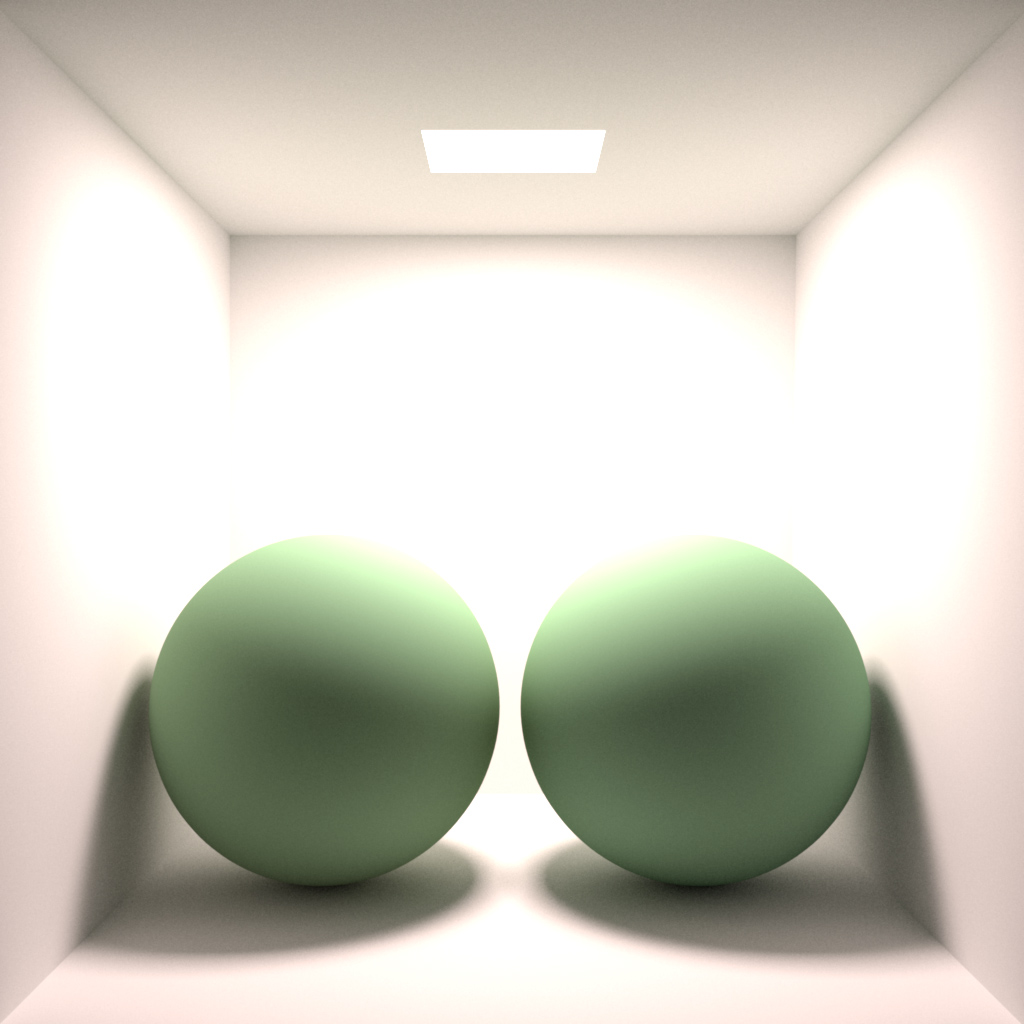
\includegraphics[alt={Illuminant E.},width=\textwidth]{mitsuba-cornellbox-metamerism-E.jpg}
        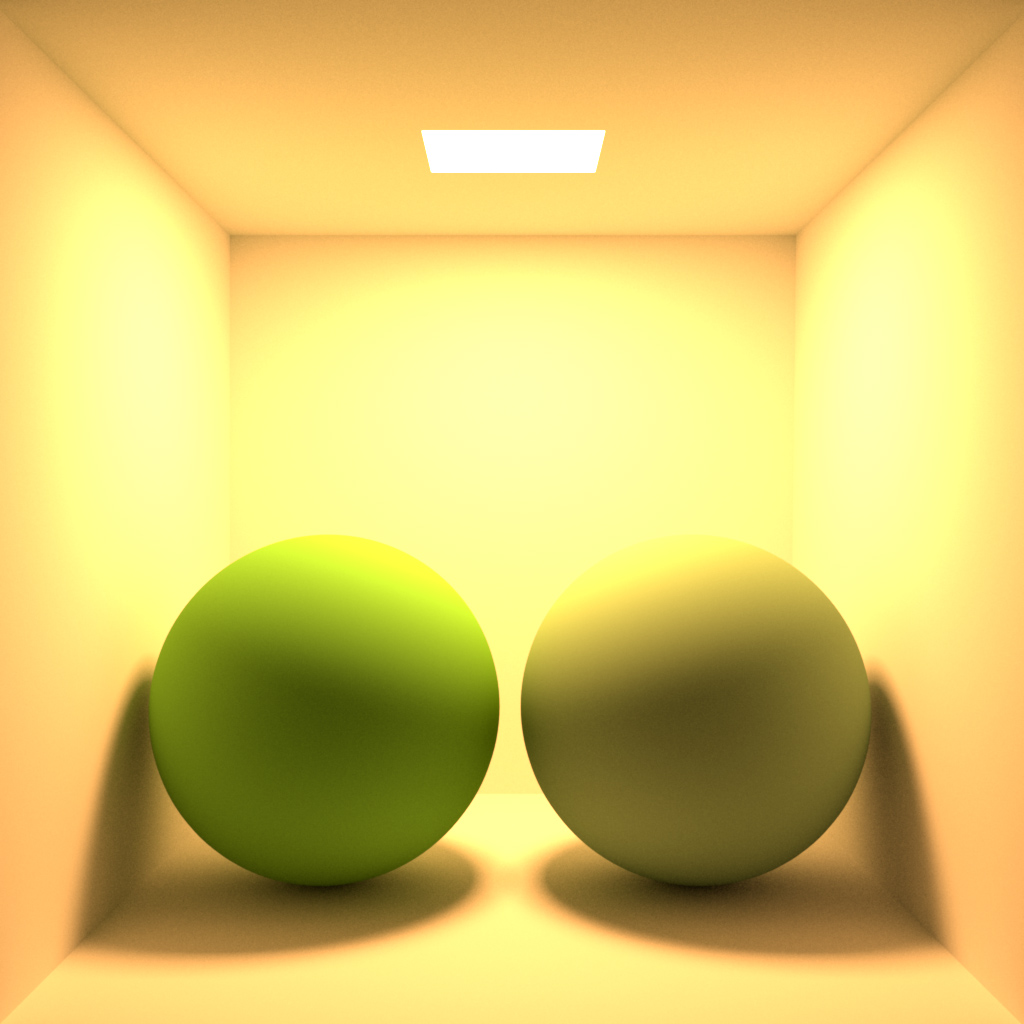
\includegraphics[alt={CIE Standard Illuminant A.},width=\textwidth]{mitsuba-cornellbox-metamerism-A.jpg}
    \fi
    \ifdefined\HCode
        \ccjericontainer{simple-jeri-embedding}
        \JavaScript
            const simpleJeriEmbeddingData = {
                title: 'Simple Jeri Embedding',
                children: [{
                        title: 'Illuminant E',
                        image: 'assets/images/mitsuba-cornellbox-metamerism-E.exr',
                    },
                    {
                        title: 'CIE Standard Illuminant A',
                        image: 'assets/images/mitsuba-cornellbox-metamerism-A.exr',
                    }
                ]
            };
            Jeri.renderViewer(document.getElementById('simple-jeri-embedding'), simpleJeriEmbeddingData);
        \EndJavaScript
    \fi
    \caption{
        Simple Jeri Embedding.
    }
    \label{fig:simple-jeri-embedding}
\end{figure}
\end{lstlisting}

\begin{figure}[H]
    \unless\ifdefined\HCode
        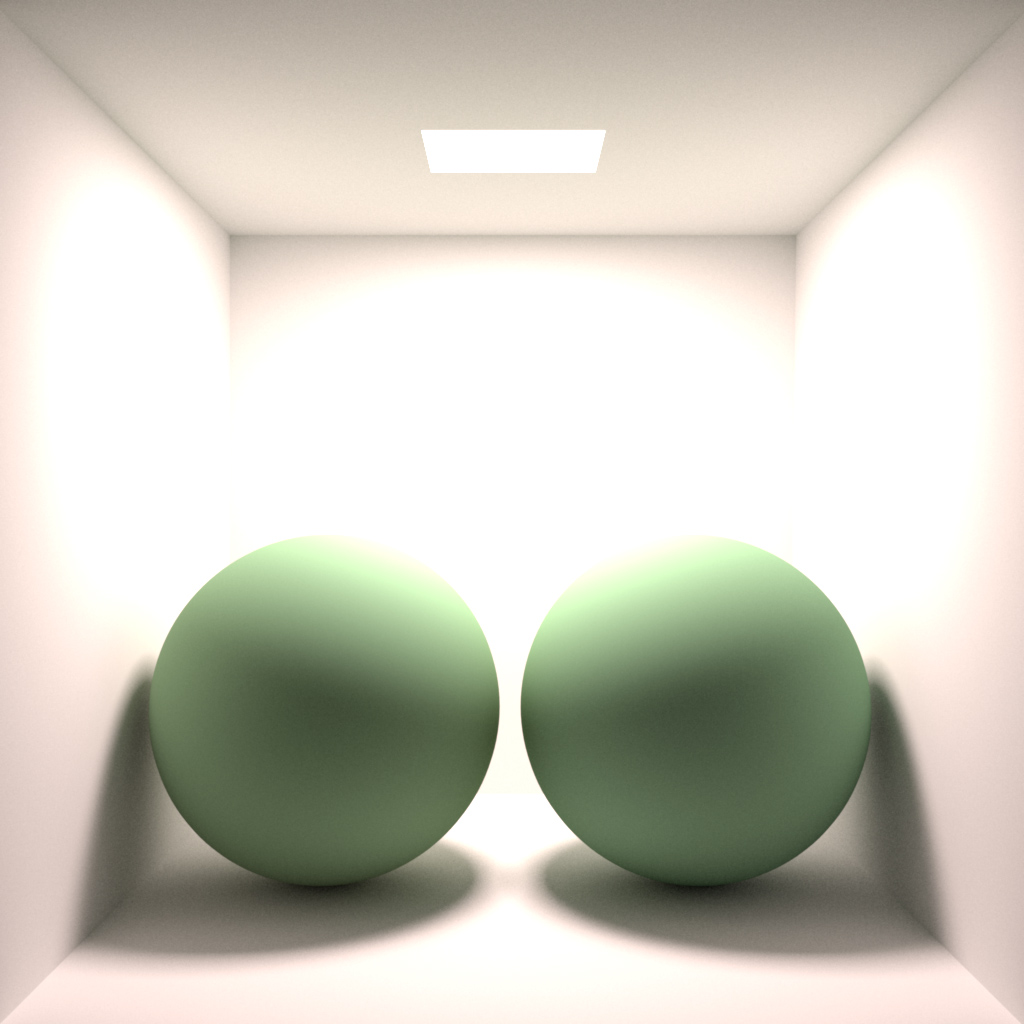
\includegraphics[alt={Illuminant E.},width=\textwidth]{mitsuba-cornellbox-metamerism-E.jpg}
        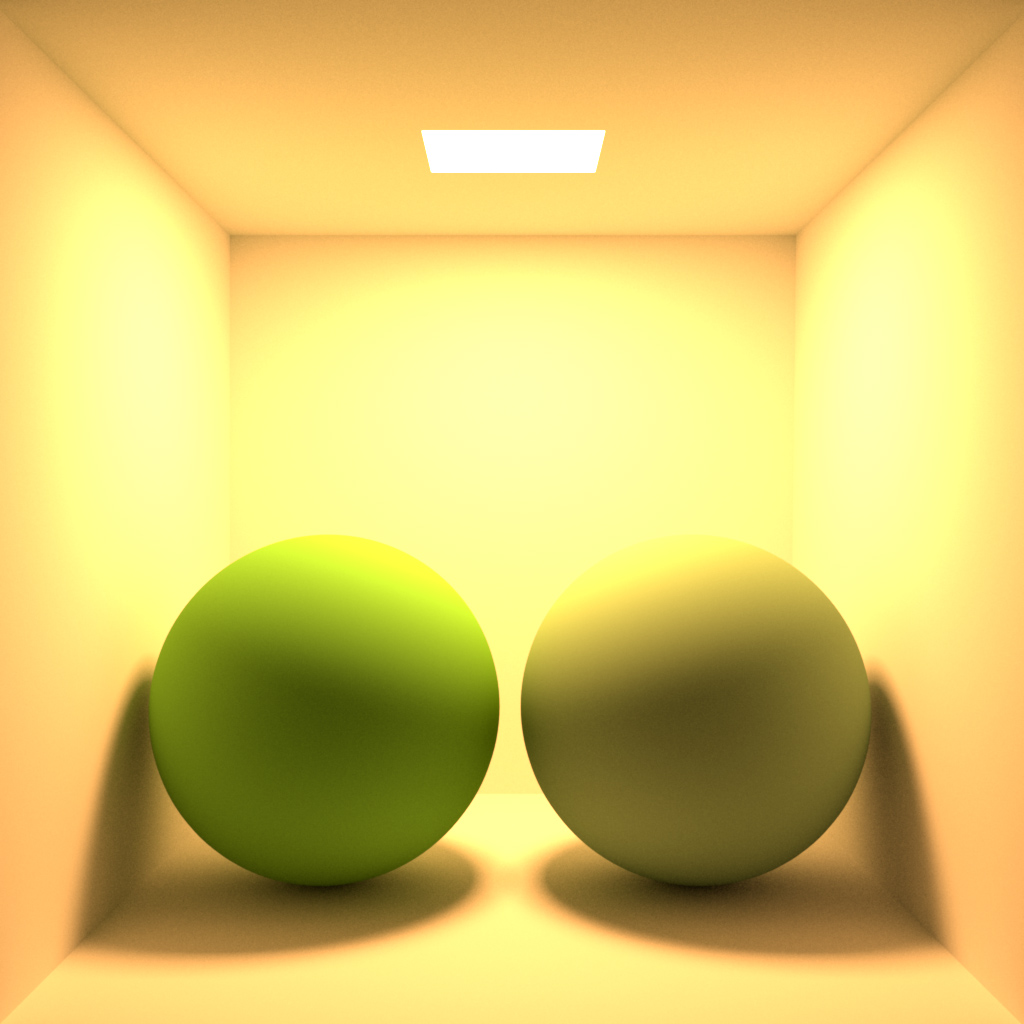
\includegraphics[alt={CIE Standard Illuminant A.},width=\textwidth]{mitsuba-cornellbox-metamerism-A.jpg}
    \fi
    \ifdefined\HCode
        \ccjericontainer{simple-jeri-embedding}
        \JavaScript
            const simpleJeriEmbeddingData = {
                title: 'Simple Jeri Embedding',
                children: [{
                        title: 'Illuminant E',
                        image: 'assets/images/mitsuba-cornellbox-metamerism-E.exr',
                    },
                    {
                        title: 'CIE Standard Illuminant A',
                        image: 'assets/images/mitsuba-cornellbox-metamerism-A.exr',
                    }
                ]
            };
            Jeri.renderViewer(document.getElementById('simple-jeri-embedding'), simpleJeriEmbeddingData);
        \EndJavaScript
    \fi
    \caption{
        Simple Jeri Embedding.
    }
    \label{fig:simple-jeri-embedding}
\end{figure}

\subsection*{Complex Jeri Embedding}

A complex \textit{Jeri} embedding example that only shows in the \textit{HTML}
output. The nested tab hierarchy has no elegant equivalent in the \textit{PDF}
output thus it not recommended to use nested tabs.

\begin{lstlisting}[caption={Complex Jeri Embedding.}]
\begin{figure}[H]
    \ifdefined\HCode
        \ccjericontainer{complex-jeri-embedding}
        \JavaScript
            const complexJeriEmbeddingData = {
                title: 'Complex Jeri Embedding',
                children: [{
                        title: 'Illuminant E',
                        image: 'assets/images/mitsuba-cornellbox-metamerism-E.exr',
                    },
                    {
                        title: 'CIE Standard Illuminant A',
                        image: 'assets/images/mitsuba-cornellbox-metamerism-A.exr',
                    },
                    {
                        title: 'Cornell Balls',
                        children: [{
                                title: 'Spectral',
                                image: 'assets/images/mitsuba-cornellbox-spectral.exr',
                            },
                            {
                                title: 'Sharp Primaries',
                                image: 'assets/images/mitsuba-cornellbox-sharp.exr',
                            }
                        ]
                    }
                ]
            };
            Jeri.renderViewer(document.getElementById('complex-jeri-embedding'), complexJeriEmbeddingData);
        \EndJavaScript
    \fi
    \caption{
        Complex Jeri Embedding.
    }
    \label{fig:complex-jeri-embedding}
\end{figure}
\end{lstlisting}

\begin{figure}[H]
    \ifdefined\HCode
        \ccjericontainer{complex-jeri-embedding}
        \JavaScript
            const complexJeriEmbeddingData = {
                title: 'Complex Jeri Embedding',
                children: [{
                        title: 'Illuminant E',
                        image: 'assets/images/mitsuba-cornellbox-metamerism-E.exr',
                    },
                    {
                        title: 'CIE Standard Illuminant A',
                        image: 'assets/images/mitsuba-cornellbox-metamerism-A.exr',
                    },
                    {
                        title: 'Cornell Balls',
                        children: [{
                                title: 'Spectral',
                                image: 'assets/images/mitsuba-cornellbox-spectral.exr',
                            },
                            {
                                title: 'Sharp Primaries',
                                image: 'assets/images/mitsuba-cornellbox-sharp.exr',
                            }
                        ]
                    }
                ]
            };
            Jeri.renderViewer(document.getElementById('complex-jeri-embedding'), complexJeriEmbeddingData);
        \EndJavaScript
    \fi
    \caption{
        Complex Jeri Embedding.
    }
    \label{fig:complex-jeri-embedding}
\end{figure}

\section*{References and Citations}
\label{sec:references-and-citations}

The \href{https://ctan.org/pkg/biblatex-apa}{biblatex-apa Reference}
package is used for references and citations.

\subsection*{Citations}
\label{subsec:citations}

\begin{lstlisting}[caption={Citation for Single Author.}]
\textcite{ARRI2012a}
\end{lstlisting}

\textcite{ARRI2012a}

\begin{lstlisting}[caption={Citation for Multiple Authors.}]
\textcite{ARRI2012a,Barlow1964}
\end{lstlisting}

\textcite{ARRI2012a,Barlow1964}

\subsection*{Citations with Parentheses}
\label{subsec:citations-with-parentheses}

\begin{lstlisting}[caption={Citation with Parentheses for Single Author.}]
\parencite{ARRI2012a}
\end{lstlisting}

\parencite{ARRI2012a}

\begin{lstlisting}[caption={Citation with Parentheses for Multiple Authors.}s]
\parencite{ARRI2012a,Barlow1964}
\end{lstlisting}

\parencite{ARRI2012a,Barlow1964}


\end{document}